

% ============================================================
%  NWU Faculty of Engineering – Final Year Project Report
%  main.tex  |  Top-level file
%
%  COMPILE:  pdflatex → biber → pdflatex → pdflatex
%            (or simply run:  latexmk -pdf main)
%
%  FOLDER STRUCTURE expected:
%    main.tex
%    NWUStyle.sty
%    NWUBack.png          <- purple NWU banner image
%    img/                 <- all figures go here
%    bib/
%      MyBib.bib          <- your BibTeX references
%    content/
%      00_abstract.tex
%      01_introduction.tex
%      02_problem_analysis.tex
%      03_literature.tex
%      04_concept.tex
%      05_preliminary.tex
%      06_detailed.tex
%      07_implementation.tex
%      08_testing.tex
%      09_conclusion.tex
%      A_ai_usage.tex
%      B_risk_register.tex
%      C_additional.tex
% ============================================================

% ── Document class ──────────────────────────────────────────
\documentclass[12pt, a4paper]{report}

\usepackage{NWUStyle} %You need the NWUStyle.sty file to be able to use this command.


% Point biblatex at your .bib file
\addbibresource{bib/MyBib.bib}


%================================================================================

% ============================================================
%    EDIT THESE FIELDS FOR YOUR PROJECT  
% ============================================================
 
% Full project title (appears large on cover)
\Title{Gantry Crane}
 
% Subtitle / report descriptor (leave blank with {} if unused)
\ReportTitle{Group 18 Engineering Design Report}
 
% Authors
\SetEERIoneRole{EERI I}
\SetEERIoneName{Jopie Roux}
\SetEERIoneNumber{50877844}

\SetEERItwoRole{EERI II}
\SetEERItwoName{Jan-Paul Smith}
\SetEERItwoNumber{50398202}

\SetMCTRoneRole{MCTR I}
\SetMCTRoneName{Romeo Mapasa}
\SetMCTRoneNumber{46011730}

\SetMCTRTwoRole{MCTR II}
\SetMCTRTwoName{Juan Fourie}
\SetMCTRTwoNumber{50128523}

\SetREIIRole{REII}
\SetREIIName{Anton Swanepoel}
\SetREIINumber{50111086}

 
% Supervisor(s) – leave blank with {} if unused
\Supervisor{}
\CoSupervisor{}           % leave {} if none
\AssistantSupervisor{}    % leave {} if none
 
% ORCID – uncomment \showorcidtrue below and fill in number
\ORCID{0000-0000-0000-0000}
%\showorcidtrue            % uncomment to display ORCID on cover
 
% Degree information
\Degree{Bachelor of Engineering}
\Discipline{School of Electrical, Electronic and Computer Engineering}
\Campus{Potchefstroom Campus}
 
% Module / assignment (for coursework reports – leave {} for FYP)
\Module{}
\Assignment{}
 
% Dates
\Date{21 November 2026}       % generic date field
\SubmissionDate{25 November 2026}
 
% Turnitin score (leave {} to omit the line)
%\TurnitinScore{}
 
% ============================================================

\begin{document}

% ── Cover page ──────────────────────────────────────────────
\MakeTitle

% ── Abstract + Keywords ─────────────────────────────────────
% ── Abstract ────────────────────────────────────────────────
% The Abstract environment (defined in NWUStyle.sty):
%   • adds "Abstract" to the TOC
%   • sets page counter to 1 with roman numerals
%   • clears the page afterwards
\begin{Abstract}{}

This report presents the design, development, and testing of a gantry crane system for the transportation of steel metal sheets along a track.

\KeyWords{Pulley; Gantry Crane; Electro-magnet; Gearbox Design}

\end{Abstract}


% ── Table of Contents / List of Figures / List of Tables ────
\MakeTOCandLOFandLOT

% ── Declaration of Originality ──────────────────────────────
%\MakeDeclaration

% ── Switch to arabic page numbers for the body ──────────────
\cleardoublepage
\pagestyle{fancy}
\pagenumbering{arabic}
\setcounter{page}{1}

%================================================================================
%BEGIN TYPING YOUR DOCUMENT - STARTING HERE.-------------------------------------
%================================================================================

%EACH CHAPTER IS TYPED IN A SEPARATE FILE. YOU CAN ADD EACH FILE INTO YOUR DOCUMENT USING THE \input COMMAND.
% MAKE SURE THE FILES ARE IN THE SAME FOLDER AS THIS MAIN FILE.

% \input{content/ExampleChapter1} %Include the contents of the file "ExampleChapter1.tex"
% \input{content/ExampleChapter2} %Include the contents of the file "ExampleChapter2.tex"
% \input{content/ExampleChapter3} %Include the contents of the file "ExampleChapter3.tex"

% ============================================================
%  CHAPTER 1 – INTRODUCTION
% ============================================================
\chapter{Introduction}
\label{ch:introduction}

This report outlines the design, development, and testing of \ldots{}

[Introduce the broader context of the project. Explain \textit{why} the
project is important and what engineering need it addresses. Keep this
concise - typically one to two pages.]

The report is structured as follows:
Chapter~\ref{ch:system-analysis} analyses the problem, outlines the background, and establishes the project requirements.
Chapter~\ref{ch:system-design} details the system architecture and functional flow across all subsystems.
Chapter~\ref{ch:interface-control} defines the interface control and responsibility allocation among the engineering roles.
Chapter~\ref{ch:design-decisions} discusses the primary design decisions and trade-offs.
Chapter~\ref{ch:test-plan} details the subsystem and integrated test plans.
Chapter~\ref{ch:system-performance} evaluates the overall system performance against specifications.
Chapter~\ref{ch:implementation-evidence} presents physical and functional implementation evidence.
Chapter~\ref{ch:conclusion} draws conclusions and identifies future work.

% ============================================================
%  CHAPTER 2 – System Analysis
% ============================================================
\chapter{System Analysis}
\label{ch:system-analysis}
This chapter describes the background of the design~\ref{sec:background}, provides the problem statement~\ref{sec:problem-statement}, discusses project objectives~\ref{sec:objectives}, as well as the system requirements~\ref{sec:requirements}.

\section{Background}
\label{sec:background}

[Describe the domain context and motivation. Explain why the problem
exists, what current approaches are insufficient, and why an engineering
solution is warranted. Cite relevant sources.]

\section{Problem Statement}
\label{sec:problem-statement}

[Clearly state the engineering problem to be solved in one or two
focused paragraphs. Avoid proposing solutions here.]

\section{Project Objectives}
\label{sec:objectives}

The objectives of this project are:
\begin{itemize}
    \item \textbf{Objective 1:} \ldots
    \item \textbf{Objective 2:} \ldots
    \item \textbf{Objective 3:} \ldots
\end{itemize}

\section{Requirements}
\label{sec:requirements}

The system requirements are based on the document
\textit{Engineering Design 2026 -- Hoisting System System
Specification}, Revision 0, dated 4 August 2026. The specification
defines the functional, performance, interface, physical, design,
environmental, and other quality requirements for the
rail-mounted gantry/trolley hoisting system.

The system comprises five work packages: MCTR I (Lateral
Movement), MCTR II (Spooling), EEII I (Drive Electronics),
EEII II (Magnetic Load Attachment), and REII (Remote Control
Dashboard). The work packages interface with a shared embedded
controller based on the ESP32-S3-WROOM-1 module and an isolated
I/O board.

The requirements below summarise the applicable system
specification. Detailed implementation requirements and
controller pin assignments are defined in the relevant work-package
scopes of work and Controller Specification.

\subsection{Functional Requirements}
\label{subsec:func-req}

The functional requirements define the operations that the system
and its constituent subsystems shall perform.

\begin{itemize}
    \item \textbf{FR1 -- Lateral movement:}
    Upon receipt of a motion command from the controller, the
    lateral movement mechanism shall move the trolley along the
    I-beam rail in the commanded direction using a commercial
    off-the-shelf (COTS) DC motor costing less than R250.
    The associated performance target is defined by PT1.

    \item \textbf{FR2 -- Position feedback:}
    The lateral movement mechanism shall report wheel position
    to the controller via quadrature encoder feedback to support
    motion profiling by REII.

    \item \textbf{FR3 -- Wheel manufacturing:}
    The lateral movement wheels shall be custom-manufactured
    by 3D printing to support the wheel wear-characterisation
    exercise.

    \item \textbf{FR4 -- Hoisting:}
    Upon receipt of a raise or lower command, the spooling
    mechanism shall drive the hoist gearbox to lift or lower
    a payload of up to 20\,kg in the commanded direction.
    The associated performance target is defined by PT2.

    \item \textbf{FR5 -- Hoist load feedback:}
    The spooling mechanism shall continuously report the
    on-hook load to the controller during operation.

    \item \textbf{FR6 -- Fail-safe braking:}
    The active brake shall engage automatically upon loss
    of drive power or command signal and shall hold the
    payload without drift.

    \item \textbf{FR7 -- Motor drive:}
    Upon receipt of gate/PWM commands from the controller,
    the drive electronics shall convert single-phase
    230\,VAC mains power to a DC bus and invert it to a
    three-phase drive for the induction motor.

    \item \textbf{FR8 -- Drive protection:}
    The drive electronics shall detect and interrupt drive
    output during shoot-through or overcurrent conditions
    to protect the switching devices from damage.

    \item \textbf{FR9 -- Drive current feedback:}
    The drive electronics shall provide a single-ended
    current-sense signal, capped below 2.048\,V, to the
    controller for firmware-based fault inference.

    \item \textbf{FR10 -- Magnetic load attachment:}
    Upon receipt of an engage command, the magnetic load
    attachment shall generate sufficient holding force
    through a three-point electromagnet to retain a payload
    of up to 20\,kg under static conditions. The associated
    performance target is defined by PT3.

    \item \textbf{FR11 -- Magnetic load indication:}
    The magnetic load attachment shall report an on-load
    indication to the controller using current-sense
    discrimination between a loaded and unloaded grip.

    \item \textbf{FR12 -- Dashboard telemetry:}
    Upon receipt of telemetry from the controller via the
    nRF24L01 link, the dashboard shall display all operational
    parameters to the operator, including position, speed,
    load, current, fault status, and grip status.

    \item \textbf{FR13 -- Dashboard control:}
    The dashboard shall provide the operator with control
    of all system operations, including lateral motion,
    hoisting, and magnet-engagement commands.

    \item \textbf{FR14 -- Independent real-time control:}
    The embedded controller shall execute its real-time
    control loop, including drive-signal generation, sensor
    acquisition, and safety interlocks, independently of
    wireless-link or dashboard availability.

    \item \textbf{FR15 -- Standalone operation:}
    For groups without computer-engineering capacity, the
    controller shall accept motion and control commands
    via UDP over its built-in Wi-Fi interface without
    requiring additional hardware.
\end{itemize}


\subsection{Performance Requirements}
\label{subsec:perf-req}

The specification defines three quantitative performance targets.
These targets are used for graduated performance assessment rather
than as binary functional pass/fail requirements.

\begin{itemize}
    \item \textbf{PT1 -- Lateral movement speed:}
    The trolley shall achieve a lateral speed of at least
    1\,m/s, measured at a distance of 1\,m from the departure
    point under unloaded conditions. Performance marks scale
    with the demonstrated speed relative to the target.

    \item \textbf{PT2 -- Hoisting performance:}
    The hoisting mechanism shall complete a 1.6\,m hoist
    stroke within 20\,s while carrying a 20\,kg payload,
    corresponding to an average hoisting rate of approximately
    80\,mm/s. Performance marks scale with the demonstrated
    hoisting rate.

    \item \textbf{PT3 -- Magnetic holding performance:}
    The magnetic load attachment shall retain a 20\,kg payload
    against a specified disturbance force. The numerical
    disturbance-force threshold remains to be determined
    through further dynamics modelling. Performance marks
    scale with the demonstrated holding performance relative
    to the eventual threshold.
\end{itemize}


\subsection{Physical Requirements}
\label{subsec:phys-req}

The physical requirements define the payload interface and
essential hardware safety provisions.

\begin{itemize}
    \item \textbf{PHY1 -- Payload interface:}
    The payload used for testing and demonstration shall have
    a flat sheet-metal attachment surface measuring
    600\,mm $\times$ 400\,mm and at least 3\,mm thick for
    engagement by the magnetic load attachment. Additional
    mass may be used to increase the total payload to a
    maximum of 20\,kg, provided the combined centre of mass
    remains centred on the attachment surface. This
    requirement does not require the general system mounting
    plate to be made from sheet metal.

    \item \textbf{PHY2 -- Hardware emergency stop:}
    The system shall include a hardware emergency-stop
    mechanism wired directly into the high-voltage (HV) bus.
    It shall be capable of removing power from the drive
    electronics independently of the software or firmware
    state.

    \item \textbf{PHY3 -- Mains protection:}
    The mains supply feeding the drive electronics shall be
    protected by a residual-current device (RCD), considering
    the combination of high-voltage wiring and outdoor
    exposure to moisture.
\end{itemize}


\subsection{Non-Functional Requirements}
\label{subsec:nonfunc-req}

In the system specification, these requirements are classified
under \textit{Other Qualities}. They address reliability,
maintainability, usability, and affordability.

\begin{itemize}
    \item \textbf{OQ1 -- Reliability:}
    Shoot-through and overcurrent protection shall be
    validated on a milled test board before construction
    of the full-scale variable-frequency drive (VFD)
    assembly.

    \item \textbf{OQ2 -- Maintainability:}
    The core controller board shall be designed as reusable,
    general-purpose laboratory infrastructure, providing
    local analogue acquisition and data logging independently
    of any single year's design problem.

    \item \textbf{OQ3 -- Usability:}
    The dashboard shall present telemetry and controls so
    that an operator can safely command the system after
    a brief orientation, without requiring specialist RF
    or embedded-systems knowledge.

    \item \textbf{OQ4 -- Affordability:}
    Component costs shall remain within the stated constraints
    for each work package, including a cost below R250 for
    the lateral-movement motor. The total system cost per
    group shall not exceed R5,000, inclusive of all
    work-package procurement.
\end{itemize}


\subsection{Design and Construction Requirements}
\label{subsec:design-req}

The following design requirements constrain the permitted
implementation choices.

\begin{itemize}
    \item \textbf{DR1 -- Lateral-movement motor:}
    The lateral-movement drive motor shall be a COTS DC motor
    costing less than R250.

    \item \textbf{DR2 -- Spooling gearbox:}
    The spooling gearbox shall not use a worm-gear configuration.
    The spooling work-package scope further specifies a
    minimum two-stage gearbox.

    \item \textbf{DR3 -- Electromagnet construction:}
    The magnetic load attachment shall not use a complete
    COTS electromagnet or solenoid. COTS core material is
    permitted, but the electromagnets must be manufactured
    as part of the project.

    \item \textbf{DR4 -- Wireless module:}
    The wireless link shall use the nRF24L01 module.

    \item \textbf{DR5 -- Embedded controller:}
    The embedded controller shall be based on the
    ESP32-S3-WROOM-1 (N8R2) module.
\end{itemize}


\subsection{Interface Requirements}
\label{subsec:interface-req}

The controller shall provide the interfaces required to
coordinate the five work packages.

\begin{itemize}
    \item \textbf{IR1 -- Drive electronics interface:}
    The controller shall provide an isolated six-line
    gate/PWM interface to EEII I for three-phase motor
    control, together with one reserve line. A current-sense
    input shall also be provided.

    \item \textbf{IR2 -- Magnetic attachment interface:}
    The controller shall provide an isolated PWM interface
    and a single-ended current-sense input of no more than
    2.048\,V to EEII II.

    \item \textbf{IR3 -- Lateral movement interface:}
    The controller shall provide direction, PWM, and
    quadrature-encoder interfaces to MCTR I.

    \item \textbf{IR4 -- Spooling interface:}
    The controller shall provide a load-cell input and
    brake-control interface to MCTR II. The load-cell
    acquisition path remains to be finalised between an
    ADS1220 differential input and a dedicated HX711.

    \item \textbf{IR5 -- Expansion interface:}
    The controller shall provide a five-pin, protocol-agnostic
    expansion header for group-specific extensions. The
    header shall be documented as a low-voltage digital-logic
    interface only.
\end{itemize}


\subsection{Environmental and Resource Requirements}
\label{subsec:environmental-req}

The system shall satisfy the following environmental and
external-resource requirements.

\begin{itemize}
    \item The system shall operate on the existing I-beam rail
    and gantry structure located outdoors on the NWU North Campus.

    \item The system shall operate outdoors under ambient
    weather conditions typical of the site, including
    temperature variation, precipitation, solar and UV
    exposure, wind, and dust. It shall also operate in the
    presence of other groups' systems on shared or adjacent
    rail infrastructure.

    \item Electrical enclosures and wiring shall provide
    protection against rain, dust, and incidental moisture.
    Exposed materials, including 3D-printed or polymer
    components, shall be selected or rated for sustained
    outdoor UV and temperature exposure over the semester.

    \item The system shall remain operational throughout the
    design, build, integration, and demonstration phases of
    the 2026 academic semester.

    \item The system shall receive electrical power through
    one dedicated single-phase, 50\,Hz, 230\,VAC mains
    supply point per group.

    \item System-level integration, including the main
    on/off switch and distribution of mains power to the
    HV bus and to the selected COTS low-voltage supplies
    of the individual work packages, shall be assigned
    to EEII I.
\end{itemize}


\subsection{Operating States and Modes}
\label{subsec:states-modes}

The system specification defines three operating states and
two operating modes.

\textbf{Operating states:}
\begin{itemize}
    \item \textbf{Idle:} The system is powered but is not
    executing a commanded motion, hoisting, or
    magnet-engagement action.

    \item \textbf{Operational:} The system is actively
    executing a commanded lateral movement, hoisting, or
    magnet-engagement function under either operating mode.

    \item \textbf{Fault / E-Stopped:} The hardware emergency
    stop has removed power from the HV bus. All motive
    functions are inhibited independently of the software
    or firmware state.
\end{itemize}

\textbf{Operating modes:}
\begin{itemize}
    \item \textbf{Dashboard-controlled:} The operator controls
    the system through the REII PC-based dashboard over the
    nRF24L01 wireless link.

    \item \textbf{Standalone:} The operator controls the system
    directly through the controller's built-in Wi-Fi/UDP
    interface, without requiring a dashboard.
\end{itemize}

At power-up, the system shall begin in the Idle state. Both
operating modes shall be available in the Operational state.
The Fault / E-Stopped state shall take precedence over either
mode and shall inhibit motive outputs regardless of the mode
active when the emergency stop was activated.


\subsection{Open Requirements and Verification}
\label{subsec:open-req-verification}

The system specification identifies the following items as
requiring further definition or implementation-level verification.

\begin{itemize}
    \item The numerical disturbance-force threshold for PT3
    remains open pending further dynamics modelling.

    \item The spooling load-cell acquisition path remains an
    implementation choice between an ADS1220 differential
    input and a dedicated HX711.

    \item The system requirements must be assigned explicit
    verification methods, including defined test procedures,
    measurement methods, and acceptance criteria.

    \item Shoot-through and overcurrent protection shall be
    validated on the milled test board before the full-scale
    VFD assembly is constructed.
\end{itemize}

Functional requirements shall be verified as pass/fail
against their stated behaviour. Performance targets PT1--PT3
shall be assessed according to the degree to which the
specified targets are achieved. Open numerical thresholds
shall not be treated as fully defined acceptance criteria
until they have been resolved.


\section{Risk Analysis}
\label{sec:risk-analysis}

The risk analysis shall identify hazards and implementation
risks associated with the mechanical, electrical, magnetic,
and control subsystems. Particular attention shall be given
to the high-voltage drive electronics, outdoor operation,
payload retention, moving mechanisms, and emergency-stop
functionality.

The risk register shall document each identified risk,
its likelihood and impact, mitigation measures, and any
residual risk following mitigation. The detailed risk
register is provided in Appendix~\ref{app:risk}.


% ============================================================
%  CHAPTER 3 – System Design
% ============================================================
\chapter{System Design}
\label{ch:system-design}
This chapter divides the work amongst 5 engineering students according to their role presented by their degree. Each of the roles are responsible for a functional section of the design. Section~\ref{sec:functional-flow} covers the functional flow diagrams of the system. Section~\ref{sec:system-architecture} gives the overview of the system design with the top-most architecture, which is then split amongst the five roles in Section~\ref{sec:functional-units} (subsections~\ref{subsec:eeri1-fu1p1} to \ref{subsec:reii-fu1p5}).

\section{Functional Flow Diagrams}
\label{sec:functional-flow}

The flow system operation runs from development, deployment, mounting, operation and maintenance until its decomission or failure as indicated in figure~\ref{fig:ffd-lifecycle}.

\begin{figure}[H]
    \centering
    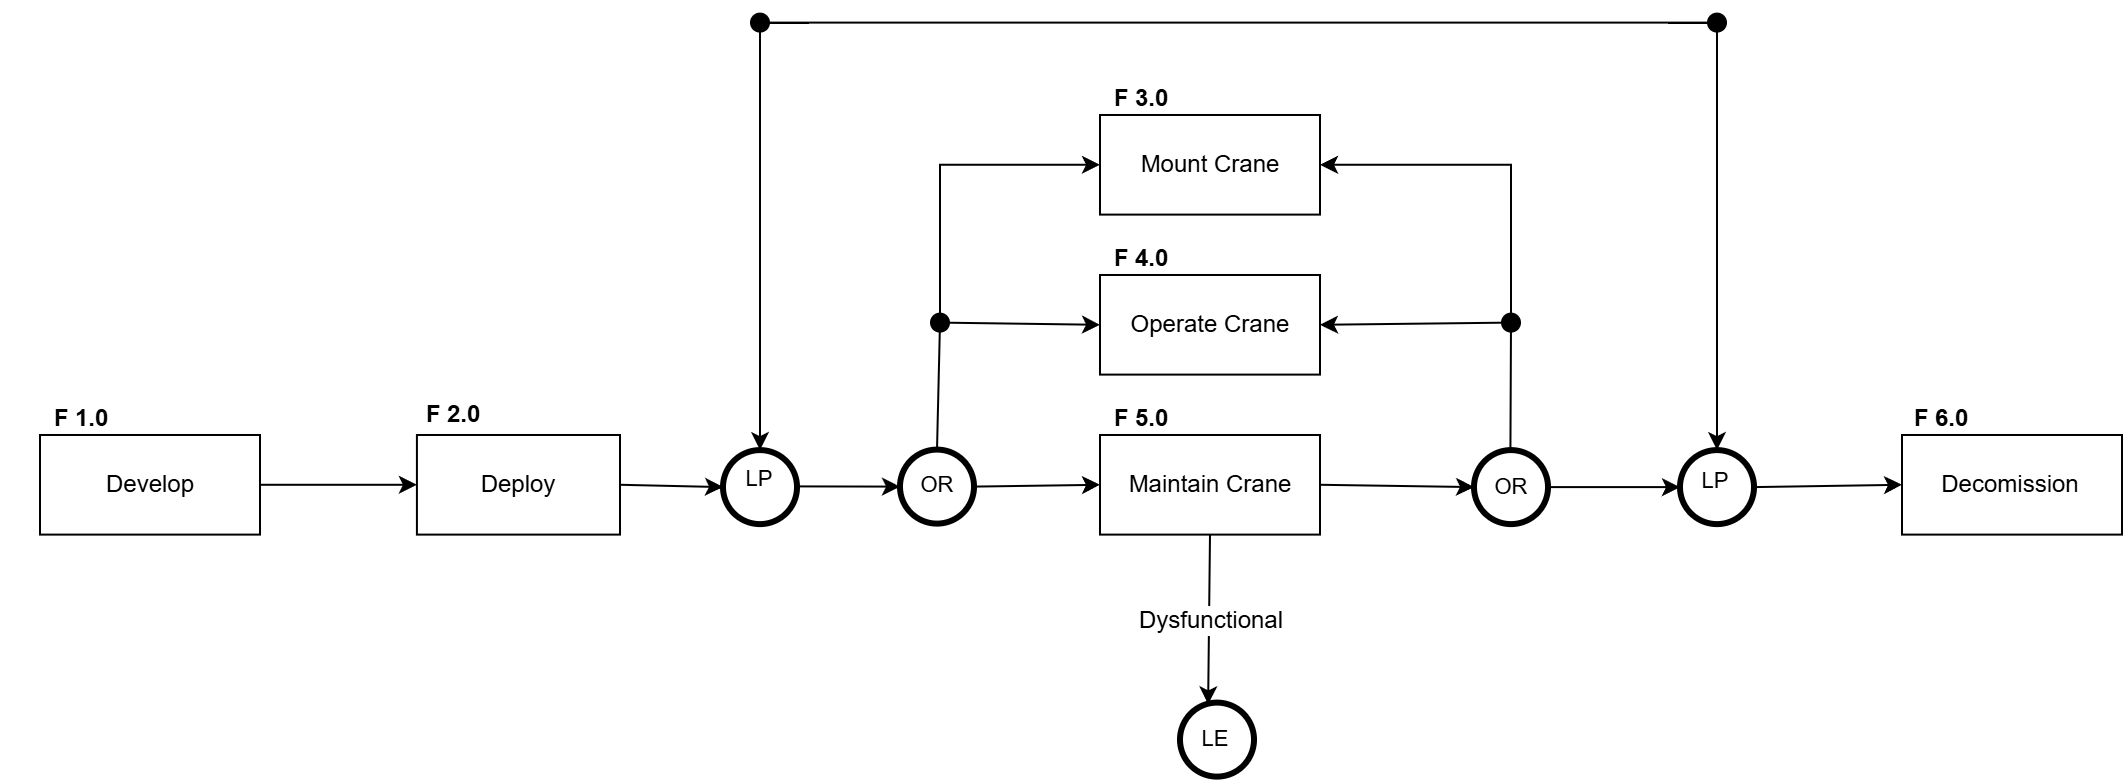
\includegraphics[width = \textwidth]{figures/Fig_LifeCycleofGantryCrane.png}
    \caption{Functional flow diagram illustrating the system life-cycle.}
    \label{fig:ffd-lifecycle}
\end{figure}

\subsection{Level 0 System Architecture}
\label{subsec:top-level-system}
The top level 0 archictecture of the system entails its interaction through the operator, support rail, power grid, environment and the payload as in figure~\ref{fig:arch-level0}

\begin{figure}[H]
    \centering
    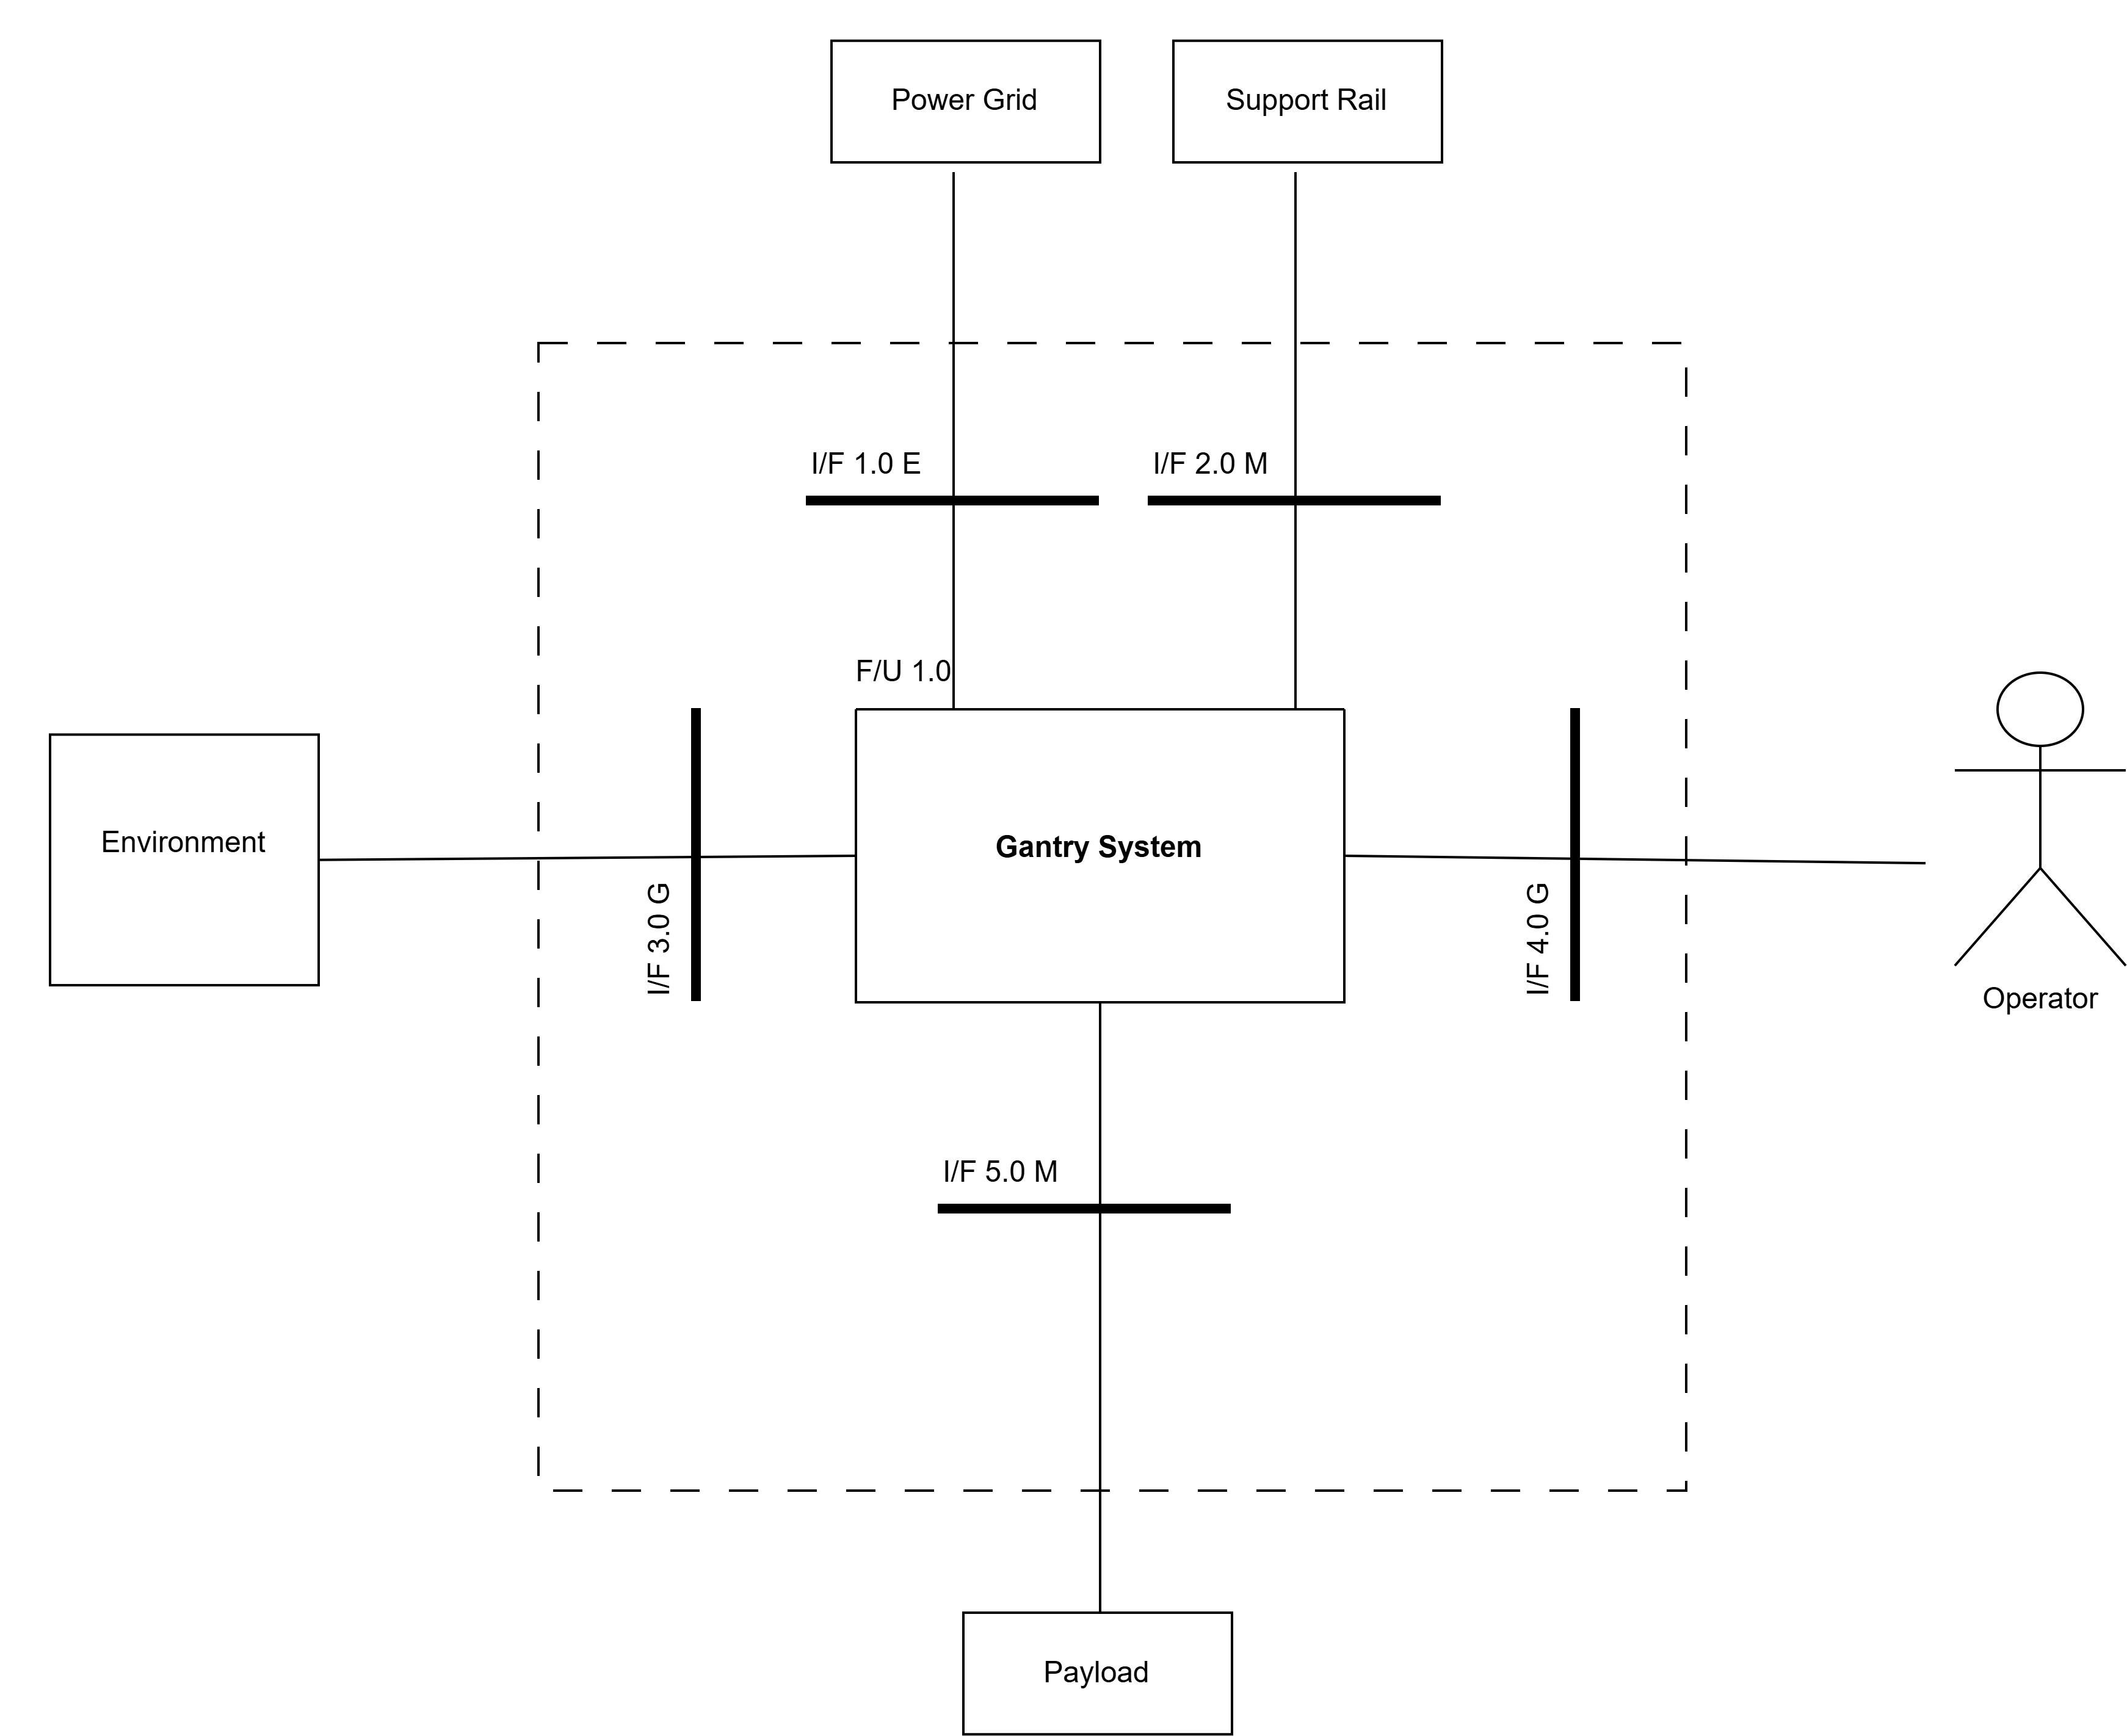
\includegraphics[width = \textwidth]{figures/Fig_Arch_Level0.png}
    \caption{System Architecture on Level 0}
    \label{fig:arch-level0}
\end{figure}

\subsection{Level 1: Gantry System F/U 1.0}
\label{subsec:gantry-system-fu}
The gantry system itself is divided up into five functional units as per the roles assigned to each group member as displayed in figure~\ref{fig:arch-level1}. Their subsequent interfaces and lower level functional units are covered by each member responsible.
\begin{figure}[H]
    \centering
    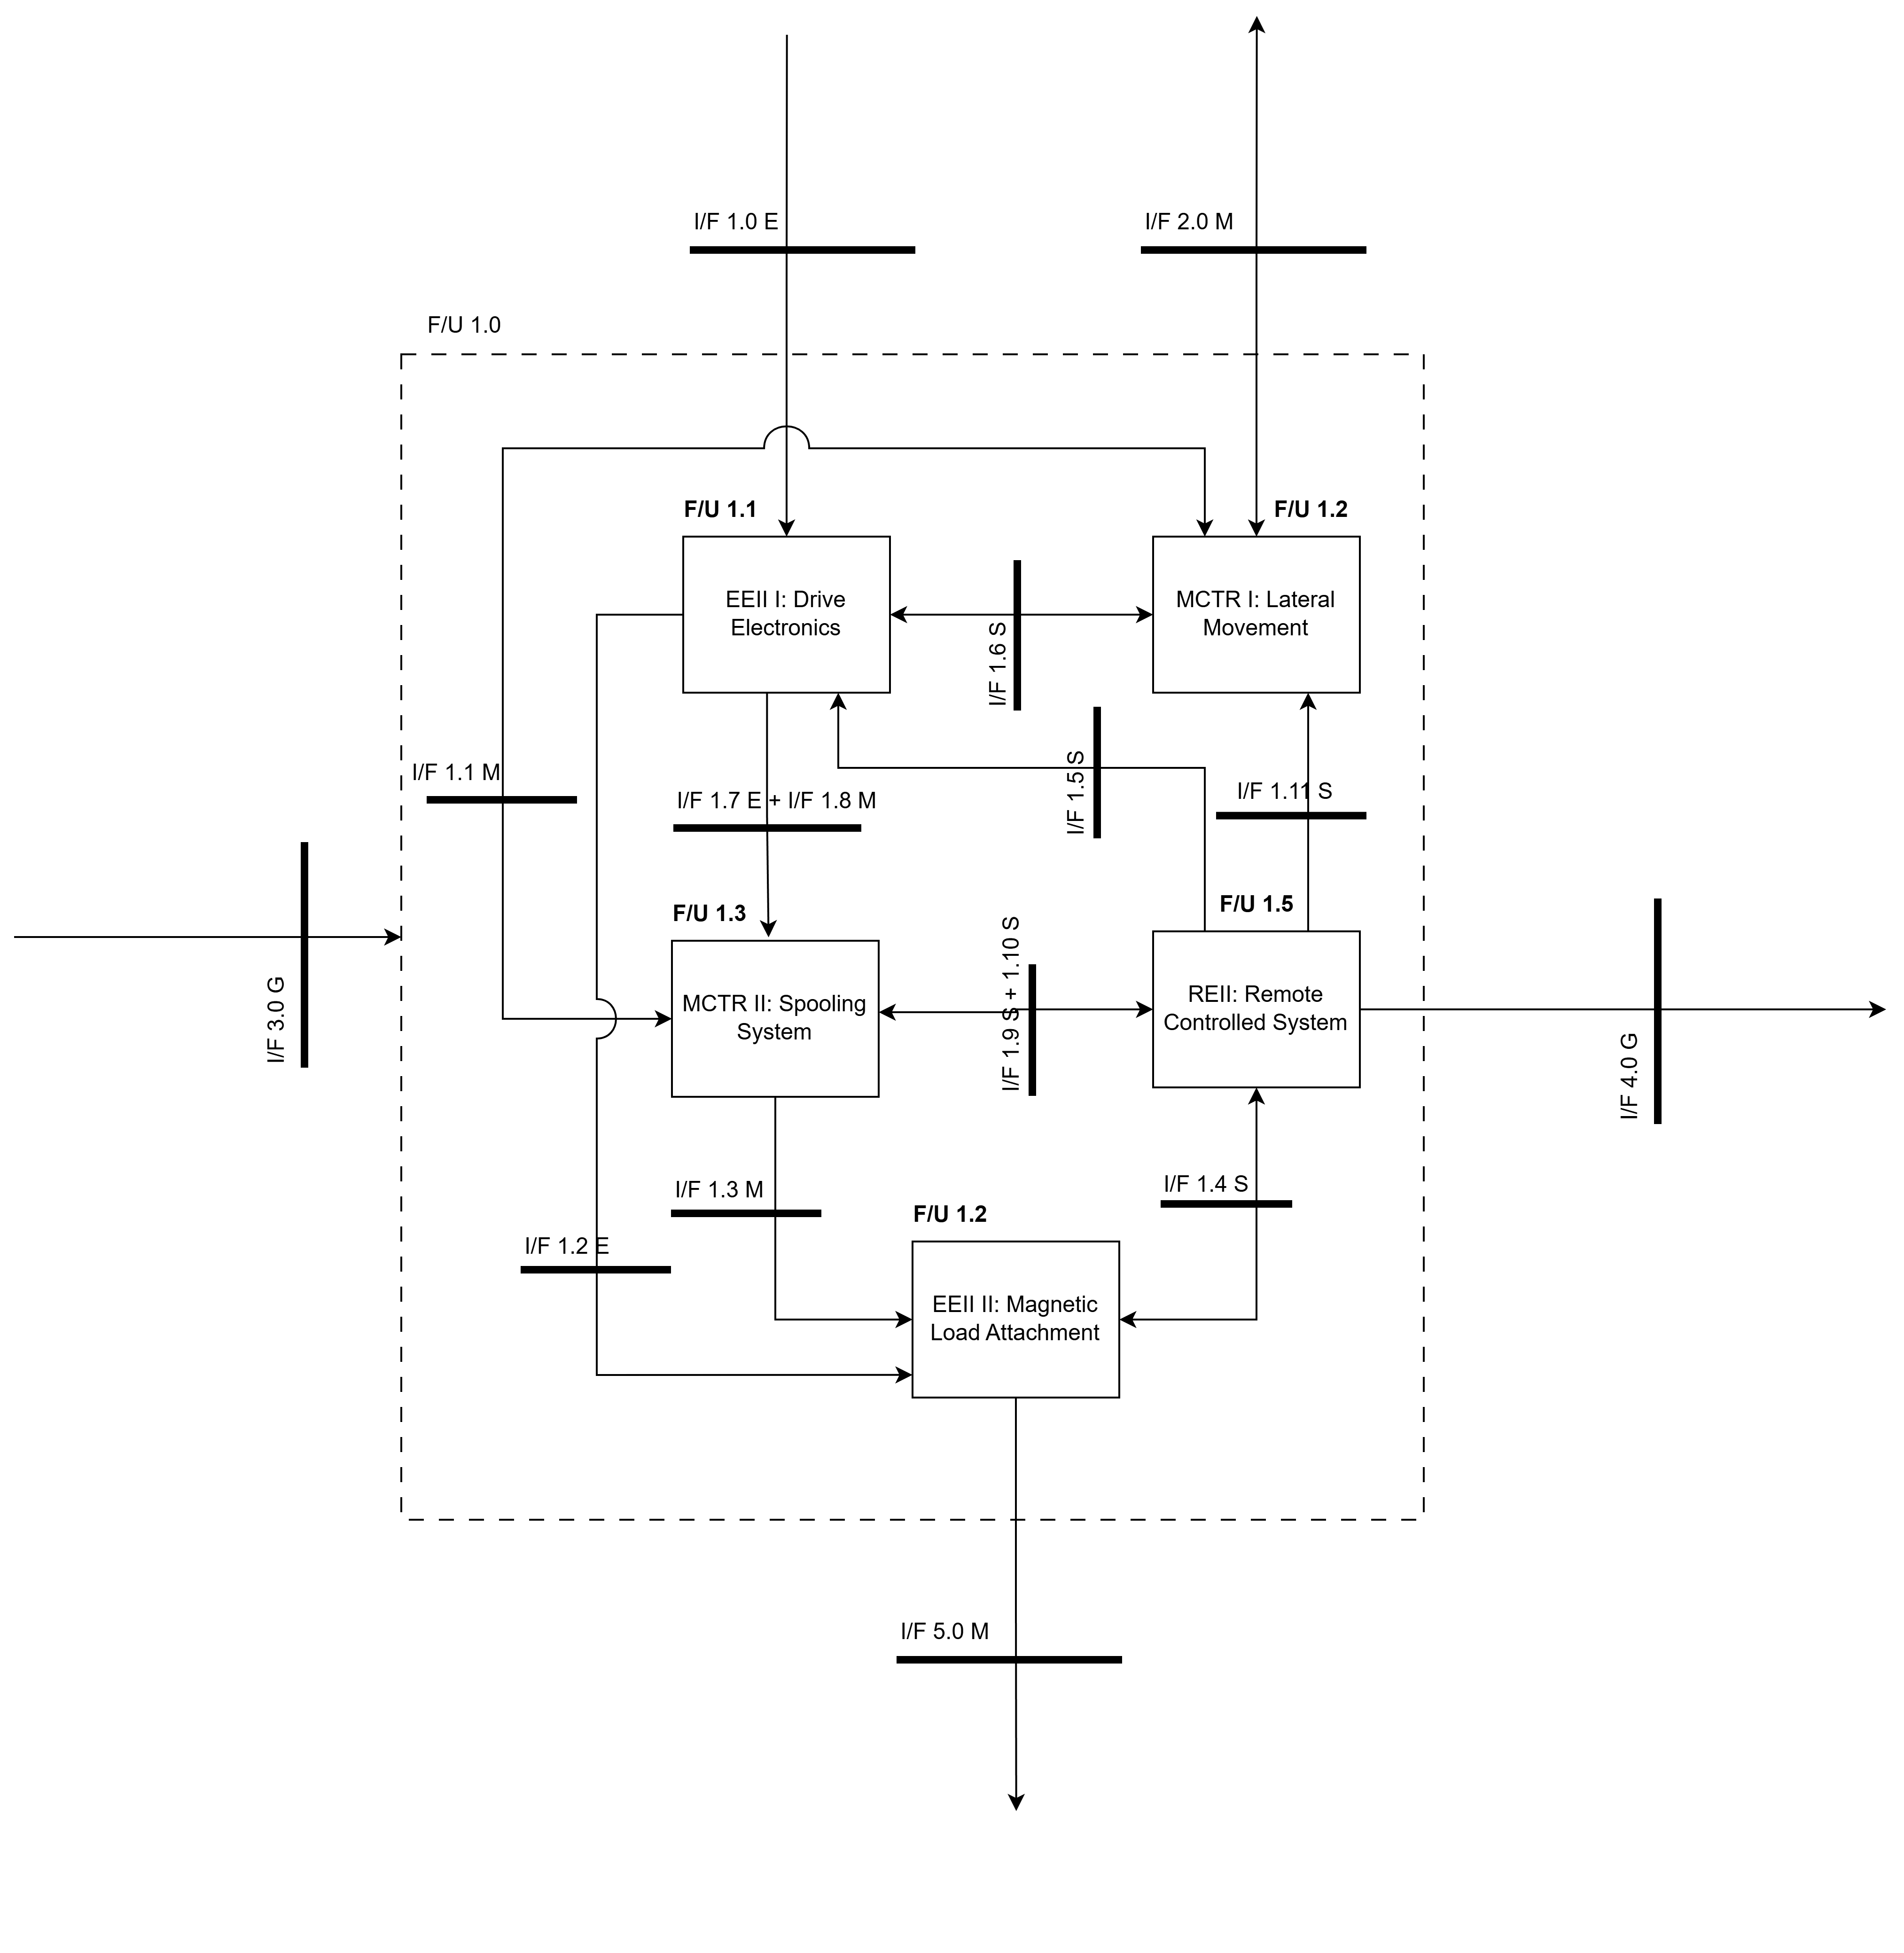
\includegraphics[width = \textwidth]{figures/Fig_Arch_Level1_GantrySystem.png}
    \caption{System Architecture on Level 1}
    \label{fig:arch-level1}
\end{figure}




\section{Level 2: Functional Units}
\label{sec:functional-units}
Each subsection handles one of the first level functional units introduced in section~\ref{sec:functional-units}.

\subsection{EERI I: Drive Electronics: F/U 1.1}
\label{subsec:eeri1-fu1p1}
EERI I Drive Electroncics by Jopie Roux.

The drive electronics subsystem converts the available single-phase 230VAC main supply to a 
controlled 3-phase supply for the induction motor. This interfaces with MCTR II through I/F 1.7 E
and 1.8 M. Figure~\ref{fig:arch-eeri1} shows the internal architecture of the subsystem and 
Table~\ref{tab:functional-units-eeri1} lists its three functional units. I additon to supplying them motor
EEII I is responsible for mains protection and distirubtion to the low voltage power supplies.
The subsystem also provides local protection against overcurrent and shoot-through conditions and
supplies current measurement feedback to the REII controller. The mains enter through I/F 1.0 E. 
The protected mains is supplied to the low voltage power supplies through I/F 1.2 E and 1.6 E. The
protected mains is also rectified and filtered to provide a DC bus for the inverter, which interfaces with
the induction motor through I/F 1.7 E. The motor interfaces mechanically with MCTR II through I/F 1.8 M.
Contorl commands are received form the REII controller through I/F 1.5 S through the isolation and gate
drivers. These control commands include the PWM signals used by the diver ICs to switch the IGBTs in the
inverter. The inverter also provides current feedback to the REII controller through I/F 1.5 S.


\begin{figure}[H]
    \centering
    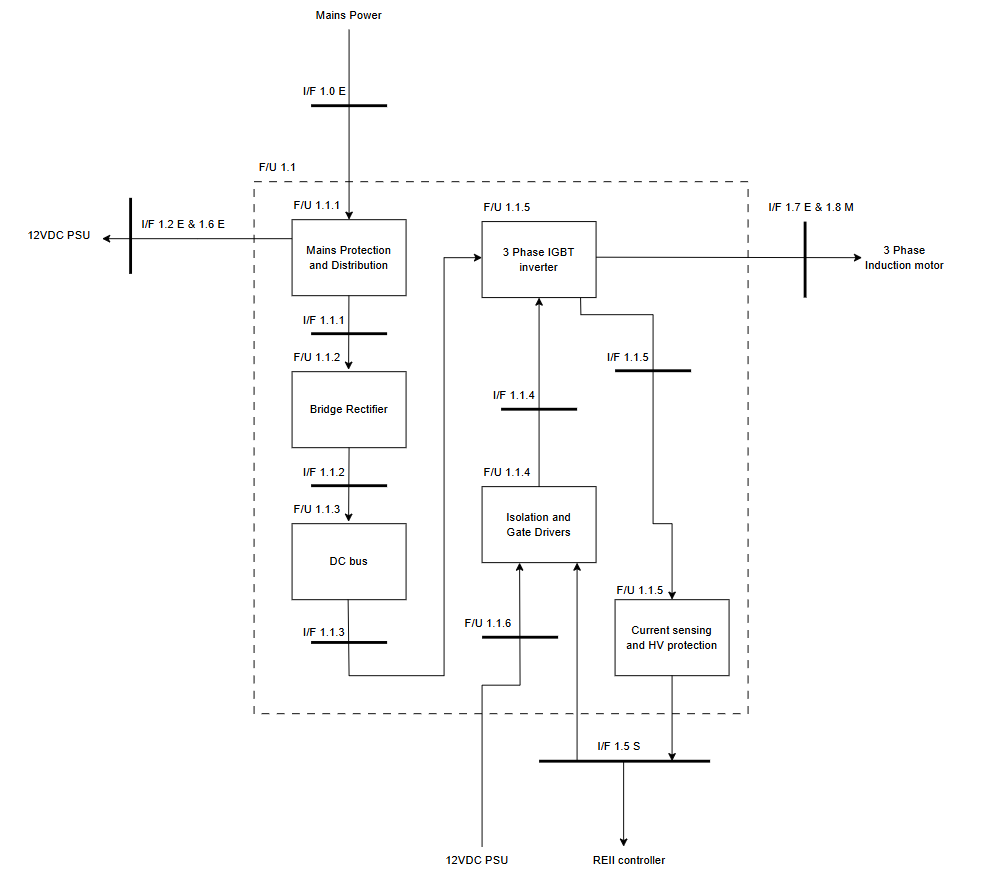
\includegraphics[width = \textwidth]{figures/Fig_Arch_Level2_EEII1.png}
    \caption{System Architecture of F/U 1.1 of the Drive Electronics Subsystem}
    \label{fig:arch-eeri1}
\end{figure}


\begin{table}[H]
    \centering
    \caption{Functional units of the EEII I drive electronics subsystem (F/U 1.1)}
    \label{tab:functional-units-eeri1}
    \begin{tabular}{@{} l l p{7cm} @{}}
        \toprule
        \textbf{F/U ID} & \textbf{Name} & \textbf{Description} \\
        \midrule
        F/U 1.1.1 & Mains Protection and Distribution
        & Receives the 230VAC mains supply and provides protected distribution to the low voltage 
        power supplies and drive electronics. This stage also contains the hardware isolation and emergency
        disconnect for high voltage applications. \\
        F/U 1.1.2 & Bridge Rectifier
         & Converts the 230VAC into a unregulated DC supply for the DC bus. \\
        F/U 1.1.3 & DC Bus
         & Smooths and stores the DC voltage for the inverter using a bulk capacitor. \\
        F/U 1.1.4 & Isolation and Gate Drivers
         & Provides electrical isolation between the REII controller and the high voltage drive electronics.
         The Driver ICs convert the incomming PWM signals into appropriate gate drive signals used to switch 
         the IGBTs in the inverter. \\
        F/U 1.1.5 & 3 Phase IGBT Inverter
         & Uses 6 IGBTs arranged in 3 half-bridges to convert DC to 3-phase AC. \\
        F/U 1.1.6 & Current sensing and HV Protection
         & Measures the drive current and provides the controller with a conditioned current feedback signal
         below 2.048V. \\
        \bottomrule
    \end{tabular}
\end{table}

\subsection{EERI II: Magnetic Load Attachment: F/U 1.2}
\label{subsec:eeri2-fu1p2}
The EERI II subsystem, engineered by J.P. Smith,
provides electromagnetic payload retention,
fast power switching and analog current sensing.
Figure~\ref{fig:arch-eeri2} shows the internal Level~2 architecture of the subsystem and its interface boundaries.
The subsystem decomposes into three lower-level functional units (Table~\ref{tab:eeri2-functional-units}).
The assembly is powered from the EEII~I $+13.5\,\text{V}$ DC bus via interface I/F~1.2~E, is suspended mechanically from the MCTR~II hoist cable hook via I/F~1.3~M,
and interfaces with the REII controller via I/F~1.10~S to receive PWM signal and transmit current signal ($V_{\mathrm{ISENSE}} \le 2.048\,\text{V}$).
The physical interface to the 20\,kg flat steel payload plate is designated as I/F~5.0~M.

\begin{figure}[H]
    \centering
    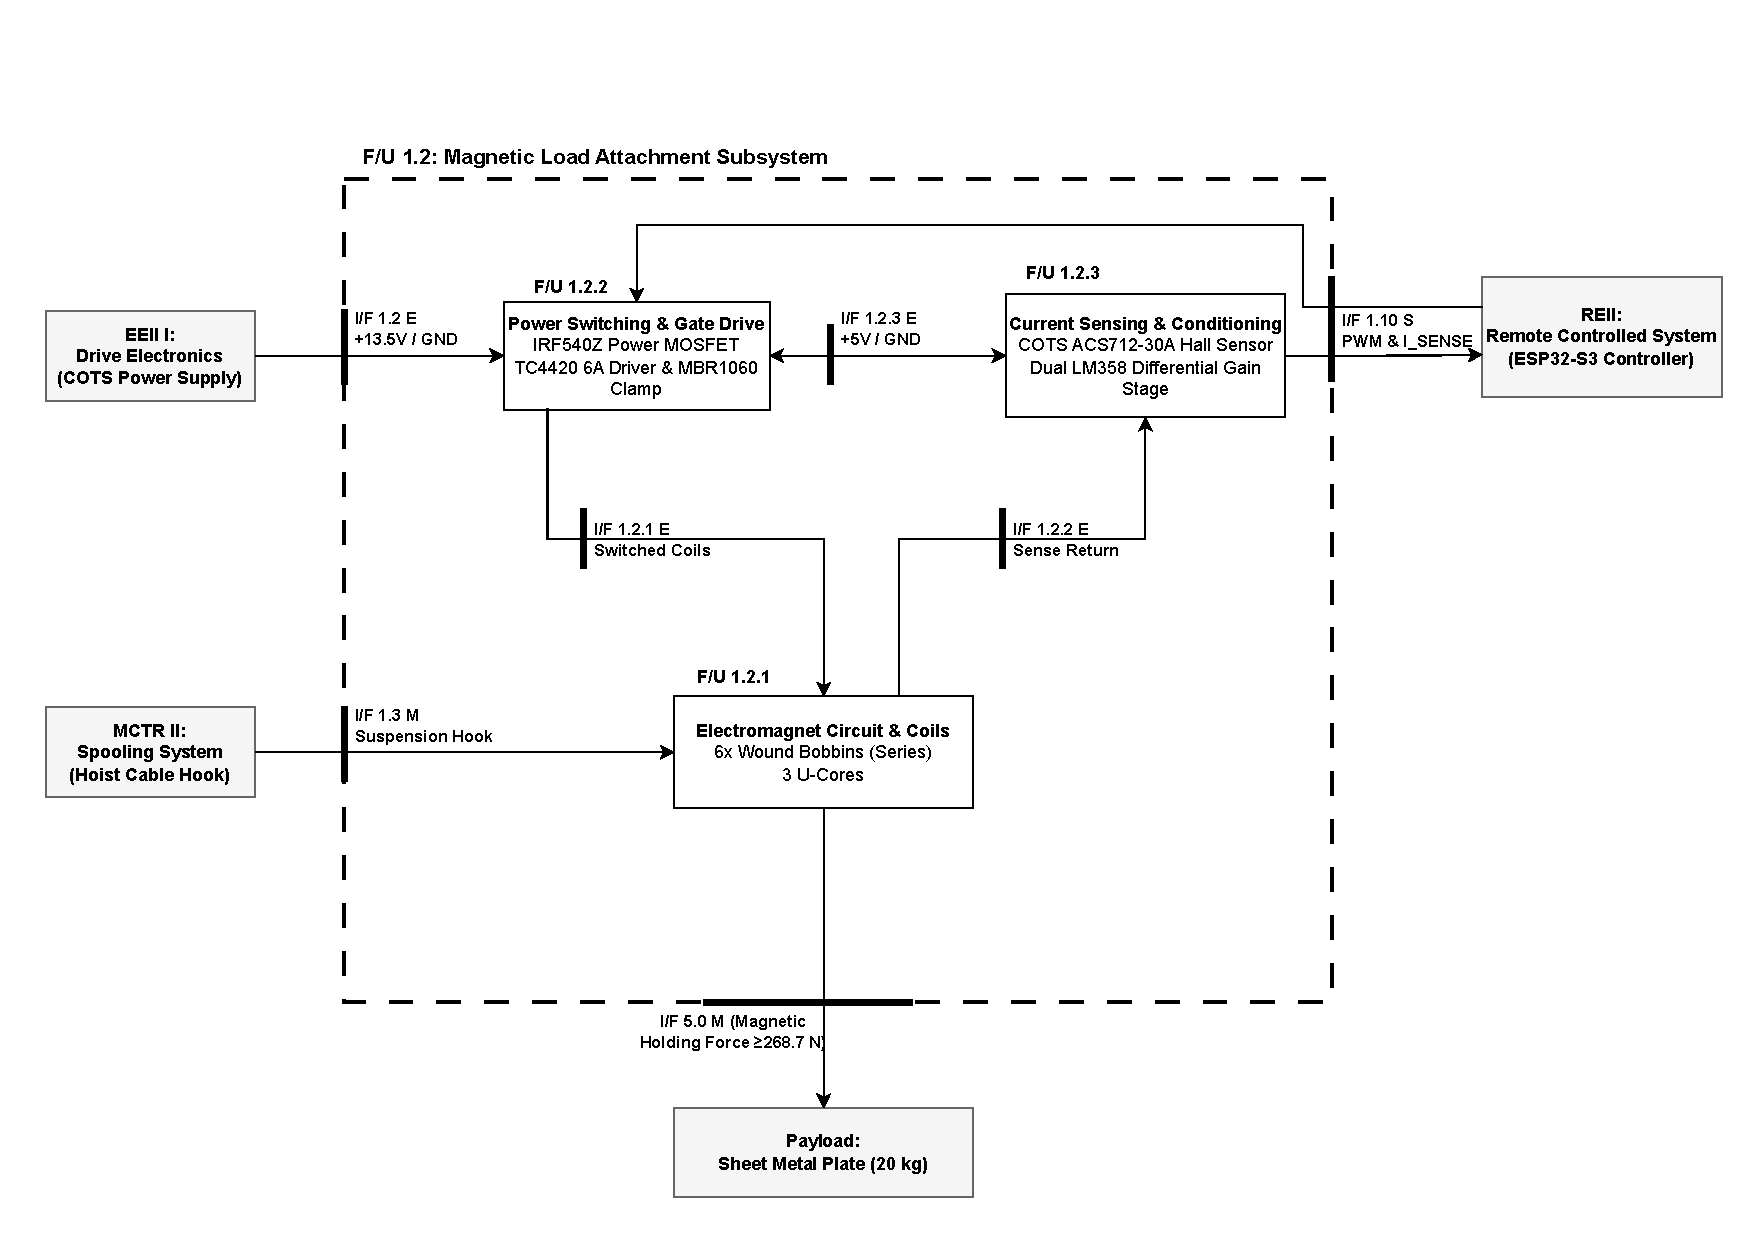
\includegraphics[width = \textwidth]{figures/JP_EEII_II_Subsystem.pdf}
    \caption{Level 2 architecture of the EERI II magnetic load attachment subsystem (F/U 1.2).}
    \label{fig:arch-eeri2}
\end{figure}

\begin{table}[H]
    \centering
    \caption{Functional units of the EERI II magnetic load attachment subsystem (F/U 1.2).}
    \label{tab:eeri2-functional-units}
    \begin{tabular}{@{} l l p{8.5cm} @{}}
        \toprule
        \textbf{F/U ID} & \textbf{Name} & \textbf{Description} \\
        \midrule
        F/U 1.2.1 & Magnetic Circuit \& Coils & Three U-core electromagnet assembly with six bobbins/legs ($28.0\,\text{m}$ of $1.00\,\text{mm}$ OD enamelled copper wire each, 286~turns/spool) providing $\ge 268.68\,\text{N}$ static holding capacity on $\ge 5\,\text{mm}$ steel plates (safety factor 1.37 on 20\,kg payload). \\
        F/U 1.2.2 & Power Switching  \& Gate Drive & High-current low-side switching using an IRF540Z  MOSFET driven by a TC4420 6\,A MOSFET driver from the $+13.5\,\text{V}$ rail, protected by an MBR1060 Schottky flyback diode. \\
        F/U 1.2.3 & Current Sensing  \& Conditioning & Galvanically isolated COTS ACS712-30A Hall-effect module conditioned via LM358 op-amp gain and offset subtraction, scaling $0\text{--}3\,\text{A}$ to $0.015\text{--}1.980\,\text{V} \le 2.048\,\text{V}$ for the REII ADC. \\
        \bottomrule
    \end{tabular}
\end{table}

\subsection{MCTR I: Lateral Movement: F/U 1.3}
\label{subsec:mctr1-fu1p3}
MCTR I Lateral Movement by Romeo Mapasa.
\begin{table}[H]
    \centering
    \caption{Operational Functional Units.}
    \label{tab:functional-units-mctr1}
    \begin{tabular}{@{} l l p{7cm} @{}}
        \toprule
        \textbf{F/U ID} & \textbf{Name} & \textbf{Description} \\
        \midrule
        F/U 1.0 & [Subsystem A] & [What this functional unit does.] \\
        F/U 2.0 & [Subsystem B] & [What this functional unit does.] \\
        F/U 3.0 & [Subsystem C] & [What this functional unit does.] \\
        \bottomrule
    \end{tabular}
\end{table}


\subsection{MCTR II: Spooling: F/U 1.4}
\label{subsec:mctr2-fu1p4}
MCTR II Spooling by Juan Fourie.
% =====================================================================
%  mctr2_parameters.tex  --  MCTR II (Spooling) parameter + calculation sheet
%
%  HOW TO USE
%   * Edit ONLY the \In... values in Section 1. Everything in Section 2
%     (\Raw... results) is computed from them by \fpeval, so every
%     table, equation and sentence that quotes a result updates on the
%     next compile.
%   * Units are noted per line. Torques in N.m unless stated.
%   * Display helpers:  \shown{Name}{digits}        -> number only
%                       \showv{Name}{digits}{unit}  -> number + unit
%   * This file is safe to \input from several chapters (loads once).
%   * Needs: LaTeX >= 2021 (\fpeval in kernel), amsmath, xcolor.
% =====================================================================
\ifdefined\MCTRIIparamsloaded\else
\def\MCTRIIparamsloaded{}

\providecommand{\tbd}[1]{\textcolor{red}{\textbf{[TBD: #1]}}}
\newcommand{\val}[2]{\ensuremath{#1\,\mathrm{#2}}}
\newcommand{\shown}[2]{\fpeval{round(\csname Raw#1\endcsname,#2)}}
\newcommand{\showv}[3]{\val{\fpeval{round(\csname Raw#1\endcsname,#2)}}{#3}}
% PASS/FAIL helpers: \passge{value}{limit} passes when value >= limit
\newcommand{\passge}[2]{\ifdim #1pt<#2pt \textcolor{red}{\textbf{FAIL}}\else\textcolor{green!45!black}{\textbf{PASS}}\fi}
\newcommand{\passle}[2]{\ifdim #1pt>#2pt \textcolor{red}{\textbf{FAIL}}\else\textcolor{green!45!black}{\textbf{PASS}}\fi}

% Functional-unit number of MCTR II (Level 1 drawing: F/U 1.4).
% NOTE: the Level 2 drawing currently labels sub-units 1.3.x; change the
% drawing to 1.4.x (or set this to 1.3 to match the drawing, but 1.3 is MCTR I).
\newcommand{\fuMII}{1.3}

% ---------------------------------------------------------------------
% 1. INPUTS  (edit these)
% ---------------------------------------------------------------------
% -- Loads, stroke, timing
\newcommand{\InMassRated}{20}    % kg   rated payload (PHY1)
\newcommand{\InMassDesign}{30}   % kg   design overload case (analysis only)
\newcommand{\InMassAttach}{2}    % kg   magnet + hook hanging on rope  [TBD: weigh]
\newcommand{\InGrav}{9.81}       % m/s^2
\newcommand{\InStroke}{1.6}      % m     hoist stroke (PT2)
\newcommand{\InTimeReq}{20}      % s     max stroke time (PT2)
\newcommand{\InServiceF}{1.5}    % -     service factor on drum torque
\newcommand{\InSFreq}{1.5}       % -     minimum acceptable safety factor (strength checks)
% -- Drum and rope
\newcommand{\InDrumD}{50}        % mm    drum core diameter (FROZEN; 70 mm entry removed)
\newcommand{\InDrumH}{60}        % mm    drum usable length
\newcommand{\InRopeD}{5}         % mm    rope diameter
\newcommand{\InRopeCentre}{1}    % 1 = tension acts at rope centre-line (D+d); 0 = old spreadsheet (D only)
% -- Motor and VSD
\newcommand{\InMotorP}{180}      % W     Askari MS632-4
\newcommand{\InMotorN}{1360}     % rpm   at rated frequency
\newcommand{\InMotorF}{50}       % Hz    rated frequency
\newcommand{\InVsdF}{50}         % Hz    frequency VSD will actually deliver  [TBD: EEII I to confirm]
% -- Gearbox (stage A = motor side, stage B = drum side)
\newcommand{\InNpA}{16}   \newcommand{\InNgA}{102}   % pinion / gear teeth, stage A
\newcommand{\InNpB}{16}   \newcommand{\InNgB}{102}   % pinion / gear teeth, stage B
\newcommand{\InModA}{1.5} \newcommand{\InModB}{2}    % mm module
\newcommand{\InFwA}{10}   \newcommand{\InFwB}{15}    % mm face width
\newcommand{\InPhi}{25}          % deg   pressure angle (use 24 if Inventor forces it; both gears of a mesh must match)
\newcommand{\InYpA}{0.296}       % Lewis form factor, pinion  (Shigley Tbl 14-2, 20 deg value: conservative for 25 deg)
\newcommand{\InYgA}{0.447}       % Lewis form factor, gear
\newcommand{\InYpB}{0.296}
\newcommand{\InYgB}{0.447}
\newcommand{\InEta}{0.95}        % -     efficiency per gear stage
\newcommand{\InSigAllow}{20}     % MPa   allowable PETG root stress [GUESS: replace with printed-coupon result / SF]
\newcommand{\InClear}{0.25}      % mm    added centre-distance clearance (printed backlash)
\newcommand{\InBed}{220}         % mm    print bed edge length [TBD: confirm printer]
% -- Shaft, hub and fastener
\newcommand{\InShaftD}{10}       % mm    shaft diameter
\newcommand{\InSpan}{100}        % mm    bearing span (centre-to-centre)
\newcommand{\InKt}{2}            % -     bending stress-concentration factor, cross-hole
\newcommand{\InKts}{2}           % -     torsion stress-concentration factor, cross-hole
\newcommand{\InSy}{250}          % MPa   yield strength  [TBD: replace with certified grade, e.g. EN8 bright bar]
\newcommand{\InBoltD}{4}         % mm    cross-bolt diameter
\newcommand{\InHubWall}{8}       % mm    hub wall length bearing on bolt
\newcommand{\InHubAllow}{20}     % MPa   allowable PETG bearing stress [GUESS]
% -- Brake
\newcommand{\InBrakeSF}{2}       % -     brake torque safety factor
\newcommand{\InBrakeRated}{0}    % N.m   datasheet holding torque; 0 = not yet known  [TBD: datasheet]
% -- Load cell and HX711
\newcommand{\InCellCap}{100}     % kg    YZC-516 rated capacity
\newcommand{\InCellSens}{2}      % mV/V  rated output [TBD: datasheet]
\newcommand{\InExc}{5}           % V     excitation (HX711 supply)
\newcommand{\InGain}{128}        % -     HX711 channel A gain
\newcommand{\InSps}{80}          % SPS   HX711 output rate (RATE pin high)
\newcommand{\InFilt}{4}          % -     samples averaged by interlock filter
\newcommand{\InNoise}{500}       % counts peak-to-peak noise [GUESS: measure with motor running]
\newcommand{\InTrip}{1.25}       % -     overload trip as multiple of (rated + attachment)
% -- Cost (R, incl. VAT and shipping, from Cost_and_Budget.xlsx)
\newcommand{\InBudget}{5000}
\newcommand{\InCostBearings}{116.24}
\newcommand{\InCostCell}{429.00}     % [CHECK: sheet unit 493.35 + 135.70 shipping = 629.05]
\newcommand{\InCostHX}{179.40}       % [CHECK: unit price 43.70]
\newcommand{\InCostPSU}{390.17}
\newcommand{\InCostBrake}{907.68}    % excluded from the sheet's own subtotal

% ---------------------------------------------------------------------
% 2. DERIVED RESULTS  (do not edit)
% ---------------------------------------------------------------------
% -- Kinematics
\newcommand{\RawDeff}{\fpeval{\InDrumD+\InRopeCentre*\InRopeD}}
\newcommand{\RawVreq}{\fpeval{\InStroke*1000/\InTimeReq}}
\newcommand{\RawWraps}{\fpeval{\InStroke*1000/(pi*\RawDeff)}}
\newcommand{\RawWrapsFit}{\fpeval{floor(\InDrumH/\InRopeD)}}
\newcommand{\RawiA}{\fpeval{\InNgA/\InNpA}}
\newcommand{\RawiB}{\fpeval{\InNgB/\InNpB}}
\newcommand{\RawiT}{\fpeval{\RawiA*\RawiB}}
\newcommand{\RawNmot}{\fpeval{\InMotorN*\InVsdF/\InMotorF}}
\newcommand{\RawNdrum}{\fpeval{\RawNmot/\RawiT}}
\newcommand{\RawVline}{\fpeval{pi*\RawDeff*\RawNdrum/60}}
\newcommand{\RawTstroke}{\fpeval{\InStroke*1000/\RawVline}}
\newcommand{\RawSpeedMargin}{\fpeval{(\RawVline/\RawVreq-1)*100}}
\newcommand{\RawiReq}{\fpeval{pi*\RawDeff*\RawNmot/(60*\RawVreq)}}
\newcommand{\RawFmin}{\fpeval{\RawVreq*60*\RawiT/(pi*\RawDeff)*\InMotorF/\InMotorN}}
% -- Drum torque, motor sizing
\newcommand{\RawFropeR}{\fpeval{\InMassRated*\InGrav}}
\newcommand{\RawFropeD}{\fpeval{\InMassDesign*\InGrav}}
\newcommand{\RawTdrR}{\fpeval{\InMassRated*\InGrav*\RawDeff/2000}}
\newcommand{\RawTdrD}{\fpeval{\InMassDesign*\InGrav*\RawDeff/2000*\InServiceF}}
\newcommand{\RawTdrSheet}{\fpeval{\InMassDesign*\InGrav*\InDrumD/2000*\InServiceF}}
\newcommand{\RawEtaGB}{\fpeval{\InEta*\InEta}}
\newcommand{\RawTmReq}{\fpeval{\RawTdrR/(\RawiT*\RawEtaGB)}}
\newcommand{\RawTmRated}{\fpeval{\InMotorP/(2*pi*\InMotorN/60)}}
\newcommand{\RawTmMargin}{\fpeval{\RawTmRated/\RawTmReq}}
\newcommand{\RawPmech}{\fpeval{\InMassRated*\InGrav*\RawVline/1000/\RawEtaGB}}
\newcommand{\RawPavail}{\fpeval{\InMotorP*\InVsdF/\InMotorF}}
% -- Gear loads (design case) and Lewis stress
\newcommand{\RawTtwo}{\fpeval{\RawTdrD/(\RawiB*\InEta)}}
\newcommand{\RawTone}{\fpeval{\RawTtwo/(\RawiA*\InEta)}}
\newcommand{\RawFtB}{\fpeval{2*\RawTtwo*1000/(\InModB*\InNpB)}}
\newcommand{\RawFtA}{\fpeval{2*\RawTone*1000/(\InModA*\InNpA)}}
\newcommand{\RawFnB}{\fpeval{\RawFtB/cosd(\InPhi)}}
\newcommand{\RawFnA}{\fpeval{\RawFtA/cosd(\InPhi)}}
\newcommand{\RawFrB}{\fpeval{\RawFtB*tand(\InPhi)}}
\newcommand{\RawSigPA}{\fpeval{\RawFtA/(\InFwA*\InModA*\InYpA)}}
\newcommand{\RawSigGA}{\fpeval{\RawFtA/(\InFwA*\InModA*\InYgA)}}
\newcommand{\RawSigPB}{\fpeval{\RawFtB/(\InFwB*\InModB*\InYpB)}}
\newcommand{\RawSigGB}{\fpeval{\RawFtB/(\InFwB*\InModB*\InYgB)}}
\newcommand{\RawSFpA}{\fpeval{\InSigAllow/\RawSigPA}}
\newcommand{\RawSFpB}{\fpeval{\InSigAllow/\RawSigPB}}
% -- Gear geometry
\newcommand{\RawDpinA}{\fpeval{\InModA*\InNpA}}
\newcommand{\RawDgearA}{\fpeval{\InModA*\InNgA}}
\newcommand{\RawDpinB}{\fpeval{\InModB*\InNpB}}
\newcommand{\RawDgearB}{\fpeval{\InModB*\InNgB}}
\newcommand{\RawDoGearA}{\fpeval{\InModA*(\InNgA+2)}}
\newcommand{\RawDoGearB}{\fpeval{\InModB*(\InNgB+2)}}
\newcommand{\RawCdA}{\fpeval{\InModA*(\InNpA+\InNgA)/2+\InClear}}
\newcommand{\RawCdB}{\fpeval{\InModB*(\InNpB+\InNgB)/2+\InClear}}
\newcommand{\RawZmin}{\fpeval{2/(sind(\InPhi)^2)}}
\newcommand{\RawDbPinB}{\fpeval{\RawDpinB*cosd(\InPhi)}}
\newcommand{\RawBedUse}{\fpeval{max(\RawDoGearA,\RawDoGearB)/\InBed*100}}
% -- Shaft (macros with arguments: #1 = payload mass kg, #2 = torque factor)
\newcommand{\Tdr}[2]{\fpeval{#1*\InGrav*\RawDeff/2*#2}}                                   % N.mm
\newcommand{\FgB}[2]{\fpeval{2*\Tdr{#1}{#2}/(\InEta*\InModB*\InNgB*cosd(\InPhi))}}        % N
\newcommand{\Msh}[2]{\fpeval{(#1*\InGrav+\FgB{#1}{#2})*\InSpan/4}}                        % N.mm
\newcommand{\SigBsh}[2]{\fpeval{32*\Msh{#1}{#2}/(pi*\InShaftD^3)}}                        % MPa
\newcommand{\Taush}[2]{\fpeval{16*\Tdr{#1}{#2}/(pi*\InShaftD^3)}}                         % MPa
\newcommand{\VMsh}[2]{\fpeval{sqrt((\InKt*\SigBsh{#1}{#2})^2+3*(\InKts*\Taush{#1}{#2})^2)}} % MPa
\newcommand{\RawFgD}{\FgB{\InMassDesign}{\InServiceF}}
\newcommand{\RawMshD}{\Msh{\InMassDesign}{\InServiceF}}
\newcommand{\RawSigBD}{\SigBsh{\InMassDesign}{\InServiceF}}
\newcommand{\RawTauD}{\Taush{\InMassDesign}{\InServiceF}}
\newcommand{\RawVMD}{\VMsh{\InMassDesign}{\InServiceF}}
\newcommand{\RawVMR}{\VMsh{\InMassRated}{1}}
\newcommand{\RawSFsD}{\fpeval{\InSy/\RawVMD}}
\newcommand{\RawSFsR}{\fpeval{\InSy/\RawVMR}}
% -- Hub / cross-bolt (design case, drum shaft)
\newcommand{\RawFside}{\fpeval{\RawTdrD*1000/\InShaftD}}
\newcommand{\RawSigHub}{\fpeval{\RawFside/(\InBoltD*\InHubWall)}}
\newcommand{\RawTauBolt}{\fpeval{\RawFside/(pi*\InBoltD^2/4)}}
\newcommand{\RawSFhub}{\fpeval{\InHubAllow/\RawSigHub}}
% -- Rated-case (20 kg, no service factor) checks for gears and hub
\newcommand{\RawLoadRatio}{\fpeval{\RawTdrR/\RawTdrD}}
\newcommand{\RawSFpAR}{\fpeval{\RawSFpA/\RawLoadRatio}}
\newcommand{\RawSFpBR}{\fpeval{\RawSFpB/\RawLoadRatio}}
\newcommand{\RawSigHubR}{\fpeval{\RawSigHub*\RawLoadRatio}}
\newcommand{\RawSFhubR}{\fpeval{\InHubAllow/\RawSigHubR}}
% -- Brake
\newcommand{\RawTholdDrum}{\fpeval{\InMassDesign*\InGrav*\RawDeff/2000}}
\newcommand{\RawTholdIn}{\fpeval{\RawTholdDrum/\RawiT}}
\newcommand{\RawBrakeReqDrum}{\fpeval{\RawTholdDrum*\InBrakeSF}}
\newcommand{\RawBrakeReqIn}{\fpeval{\RawTholdIn*\InBrakeSF}}
\newcommand{\BrakeMarginIn}{\ifdim\InBrakeRated pt=0pt\tbd{datasheet torque}\else\fpeval{round(\InBrakeRated/\RawBrakeReqIn,1)}\fi}
\newcommand{\BrakeMarginDrum}{\ifdim\InBrakeRated pt=0pt\tbd{datasheet torque}\else\fpeval{round(\InBrakeRated/\RawBrakeReqDrum,1)}\fi}
% -- Load cell and HX711
\newcommand{\RawFcell}{\fpeval{(\InMassRated+\InMassAttach)*\InGrav}}
\newcommand{\RawMtrip}{\fpeval{(\InMassRated+\InMassAttach)*\InTrip}}
\newcommand{\RawCellUse}{\fpeval{\RawMtrip/\InCellCap*100}}
\newcommand{\RawSigFS}{\fpeval{\InCellSens*\InExc}}
\newcommand{\RawAdcRange}{\fpeval{0.5*\InExc/\InGain*1000}}
\newcommand{\RawCntPerKg}{\fpeval{\InCellSens/1000/\InCellCap*\InGain/0.5*2^23}}
\newcommand{\RawResG}{\fpeval{\InNoise/\RawCntPerKg*1000}}
\newcommand{\RawLatency}{\fpeval{\InFilt/\InSps*1000}}
\newcommand{\RawTravel}{\fpeval{\RawVline*\RawLatency/1000}}
% -- Cost
\newcommand{\RawCostTot}{\fpeval{\InCostBearings+\InCostCell+\InCostHX+\InCostPSU+\InCostBrake}}
\newcommand{\RawBudgetLeft}{\fpeval{\InBudget-\RawCostTot}}
\newcommand{\RawBudgetUse}{\fpeval{\RawCostTot/\InBudget*100}}
\fi

The spooling subsystem raises and lowers the payload on a rope wound onto a
drum, holds it safely when unpowered, and reports the on-hook load to the
controller. Figure~\ref{fig:arch-mctr2} shows its internal architecture and
Table~\ref{tab:fu-mctr2} lists its six functional units. The induction motor
that drives the gearbox is supplied and powered by EEII~I and enters this
subsystem through interface I/F~1.7~E and I/F~1.8~M. The gearbox and spool itself is mounted to the frame of MCTR~I through I/F~1.1~M. The brake signal is received from REII through I/F~1.9~S and the load cell telemetry with the power and ground required by the HX711 is sent and received by REII through I/F~1.10~S. EERI~II has its electromagnet and electrical/signal wiring connected through I/F~1.3~M.
(Chapter~\ref{ch:interface-control}).

\begin{figure}[H]
    \centering
    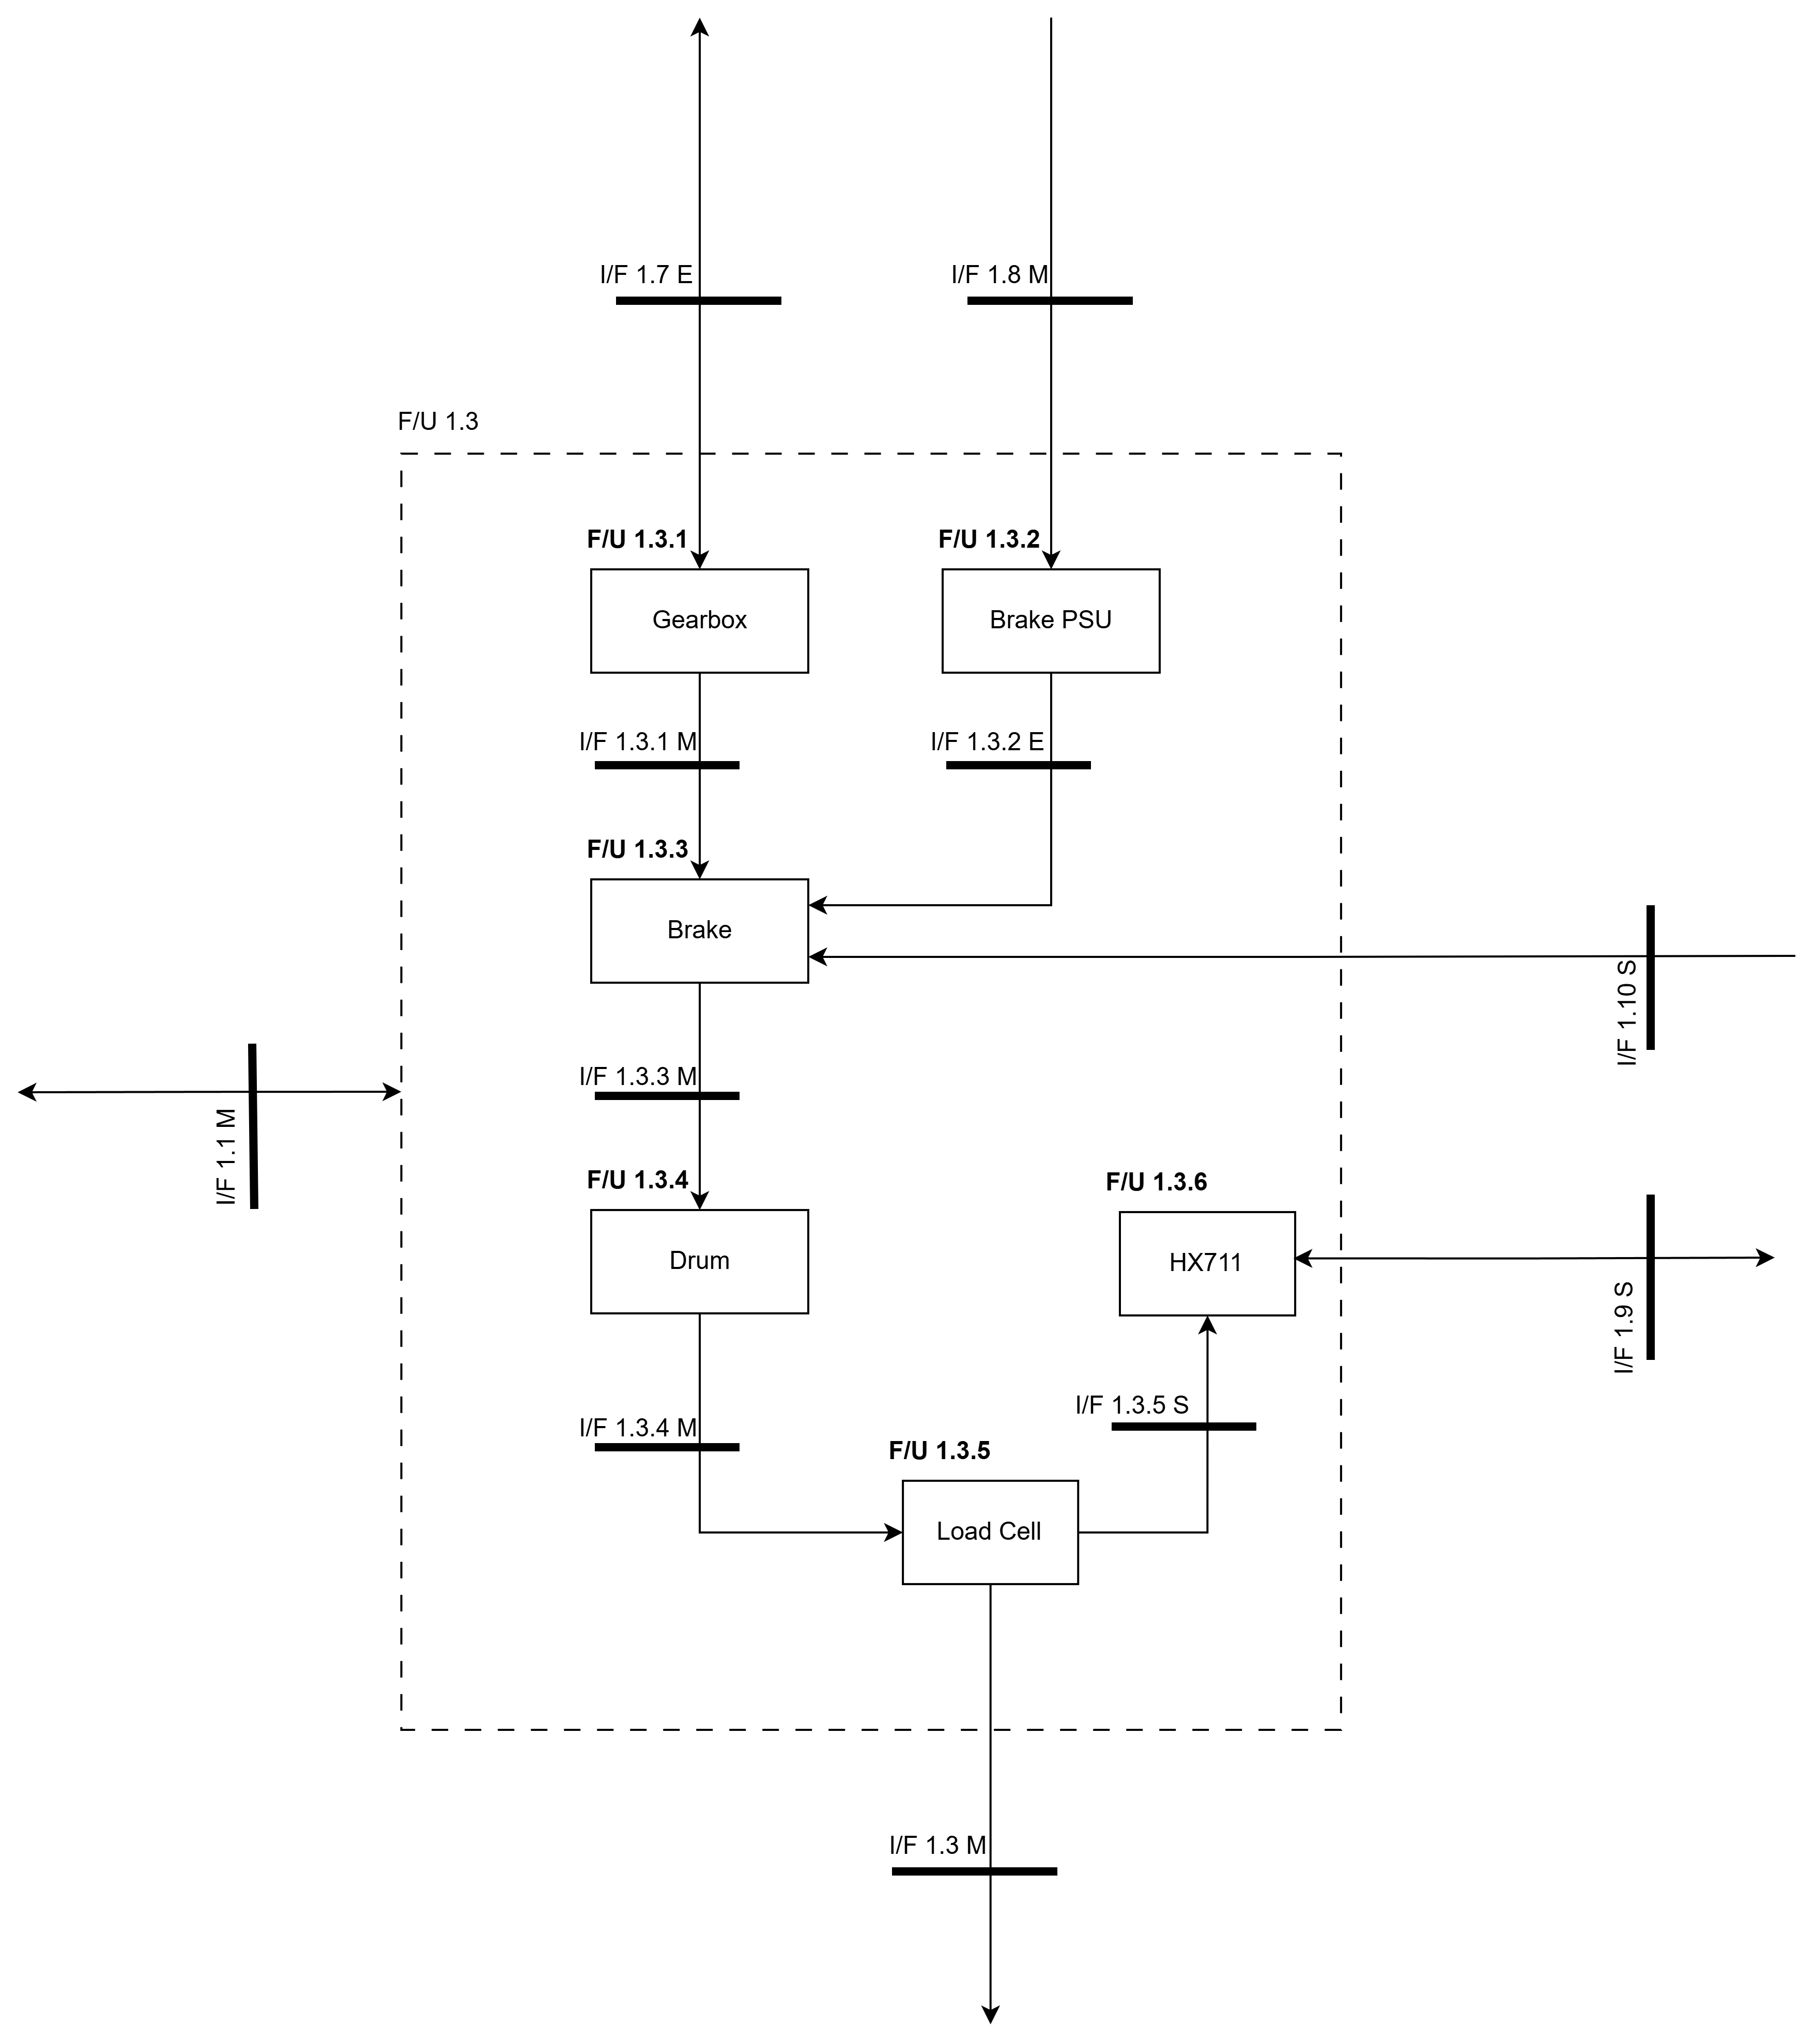
\includegraphics[width = \textwidth]{figures/Fig_Arch_Level2_MCTRII.png}
    \caption{System Architecture of F/U 1.4 of the Spooling Subsystem}
    \label{fig:arch-mctr2}
\end{figure}

\begin{table}[H]
    \centering
      \caption{Functional units of the MCTR II spooling subsystem (F/U \fuMII).}
    \label{tab:fu-mctr2}
    \small
    \begin{tabularx}{\textwidth}{@{} l l X @{}}
        \toprule
        \textbf{F/U ID} & \textbf{Name} & \textbf{Description} \\
        \midrule
        F/U \fuMII.1 & Gearbox &
            Two-stage compound spur gearbox (3D-printed PETG, no worm gear,
            DR2). Reduces motor speed (\showv{Nmot}{0}{rpm}) by an overall
            ratio of \shown{iT}{2}:1 to \showv{Ndrum}{1}{rpm} at the drum and
            multiplies motor torque to \showv{TdrR}{2}{N\,m} (rated load). \\
        F/U \fuMII.2 & Brake PSU &
            Stand-alone 48\,V DC supply for the brake coil, fed from the
            mains distribution provided by EEII~I. Switched through a relay
            that defaults to the de-energised state. \\
        F/U \fuMII.3 & Brake &
            Spring-applied, electrically released holding brake. Engages
            automatically on loss of power or command and holds the payload
            without drift (FR6). \\
        F/U \fuMII.4 & Drum &
            \InDrumD\,mm drum carrying \InRopeD\,mm rope in a single layer
            (\shown{Wraps}{1} wraps for the \InStroke\,m stroke, capacity
            \shown{WrapsFit}{0} wraps). Output shaft of the gearbox drives it
            through a hub with a cross-bolt. \\
        F/U \fuMII.5 & Load cell &
            S-type load cell (\InCellCap\,kg) carrying a sheave through which
            the rope passes; measures the on-hook load for telemetry and
            overload interlock (FR5). \\
        F/U \fuMII.6 & HX711 &
            24-bit bridge ADC converting the load-cell signal to a 2-wire
            digital stream (\InSps\,SPS) for the controller. \\
        \bottomrule
    \end{tabularx}
\end{table}

\subsection{REII: Remote Control Dashboard: F/U 1.5}
\label{subsec:reii-fu1p5}
REII Remote Control Dashboard by Anton Swanepoel

The proposed REII subsystem would provide crane commands and display
lateral position, speed, load, current, fault and the current grip status.
Figure~\ref{fig:reii-architecture} shows the architecture;
Table~\ref{tab:functional-units-reii} lists five functional units.
Commands would pass from the Python dashboard through the STM32 UART
ground station and nRF24 radios to the ESP32-S3; telemetry would return
along this path. \cite{nwu_sysrs2026,nwu_reii_scope2026}

I/F~1.5.4 would link the controller to EERI~I's inverter, while
I/F~1.5.5 would connect it to EERI~II's magnet. Both would return
current feedback for fault or grip inference. MCTR~I would receive
lateral commands and return encoder feedback through I/F~1.5.6.
Through I/F~1.5.7, REII would command MCTR~II's brake, power the HX711,
drive SCK and read DAT. Chapter~\ref{ch:interface-control} details these
interfaces. Final integration remains incomplete.
\cite{nwu_sysrs2026,nwu_reii_scope2026,nwu_s3_board2026}

\begin{table}[H]
    \centering
    \caption{Operational functional units of REII.}
    \label{tab:functional-units-reii}
    \begin{tabularx}{\textwidth}{@{}
        l
        >{\raggedright\arraybackslash}p{4cm}
        >{\raggedright\arraybackslash}X
    @{}}
        \toprule
        \textbf{F/U ID} & \textbf{Name} & \textbf{Description} \\
        \midrule
        F/U~1.5.1 & Python dashboard &
        Accept operator commands and display telemetry and faults. \\

        F/U~1.5.2 & STM32 ground station &
        Transfer messages between the PC serial connection and the radio. \\

        F/U~1.5.3 & Ground radio &
        Send commands and receive controller replies. \\

        F/U~1.5.4 & Hoist radio &
        Receive commands and return results and telemetry. \\

        F/U~1.5.5 & ESP32-S3 controller &
        Check requests, generate control outputs and collect subsystem data. \\
        \bottomrule
    \end{tabularx}
\end{table}

\begin{figure}[H]
    \centering
    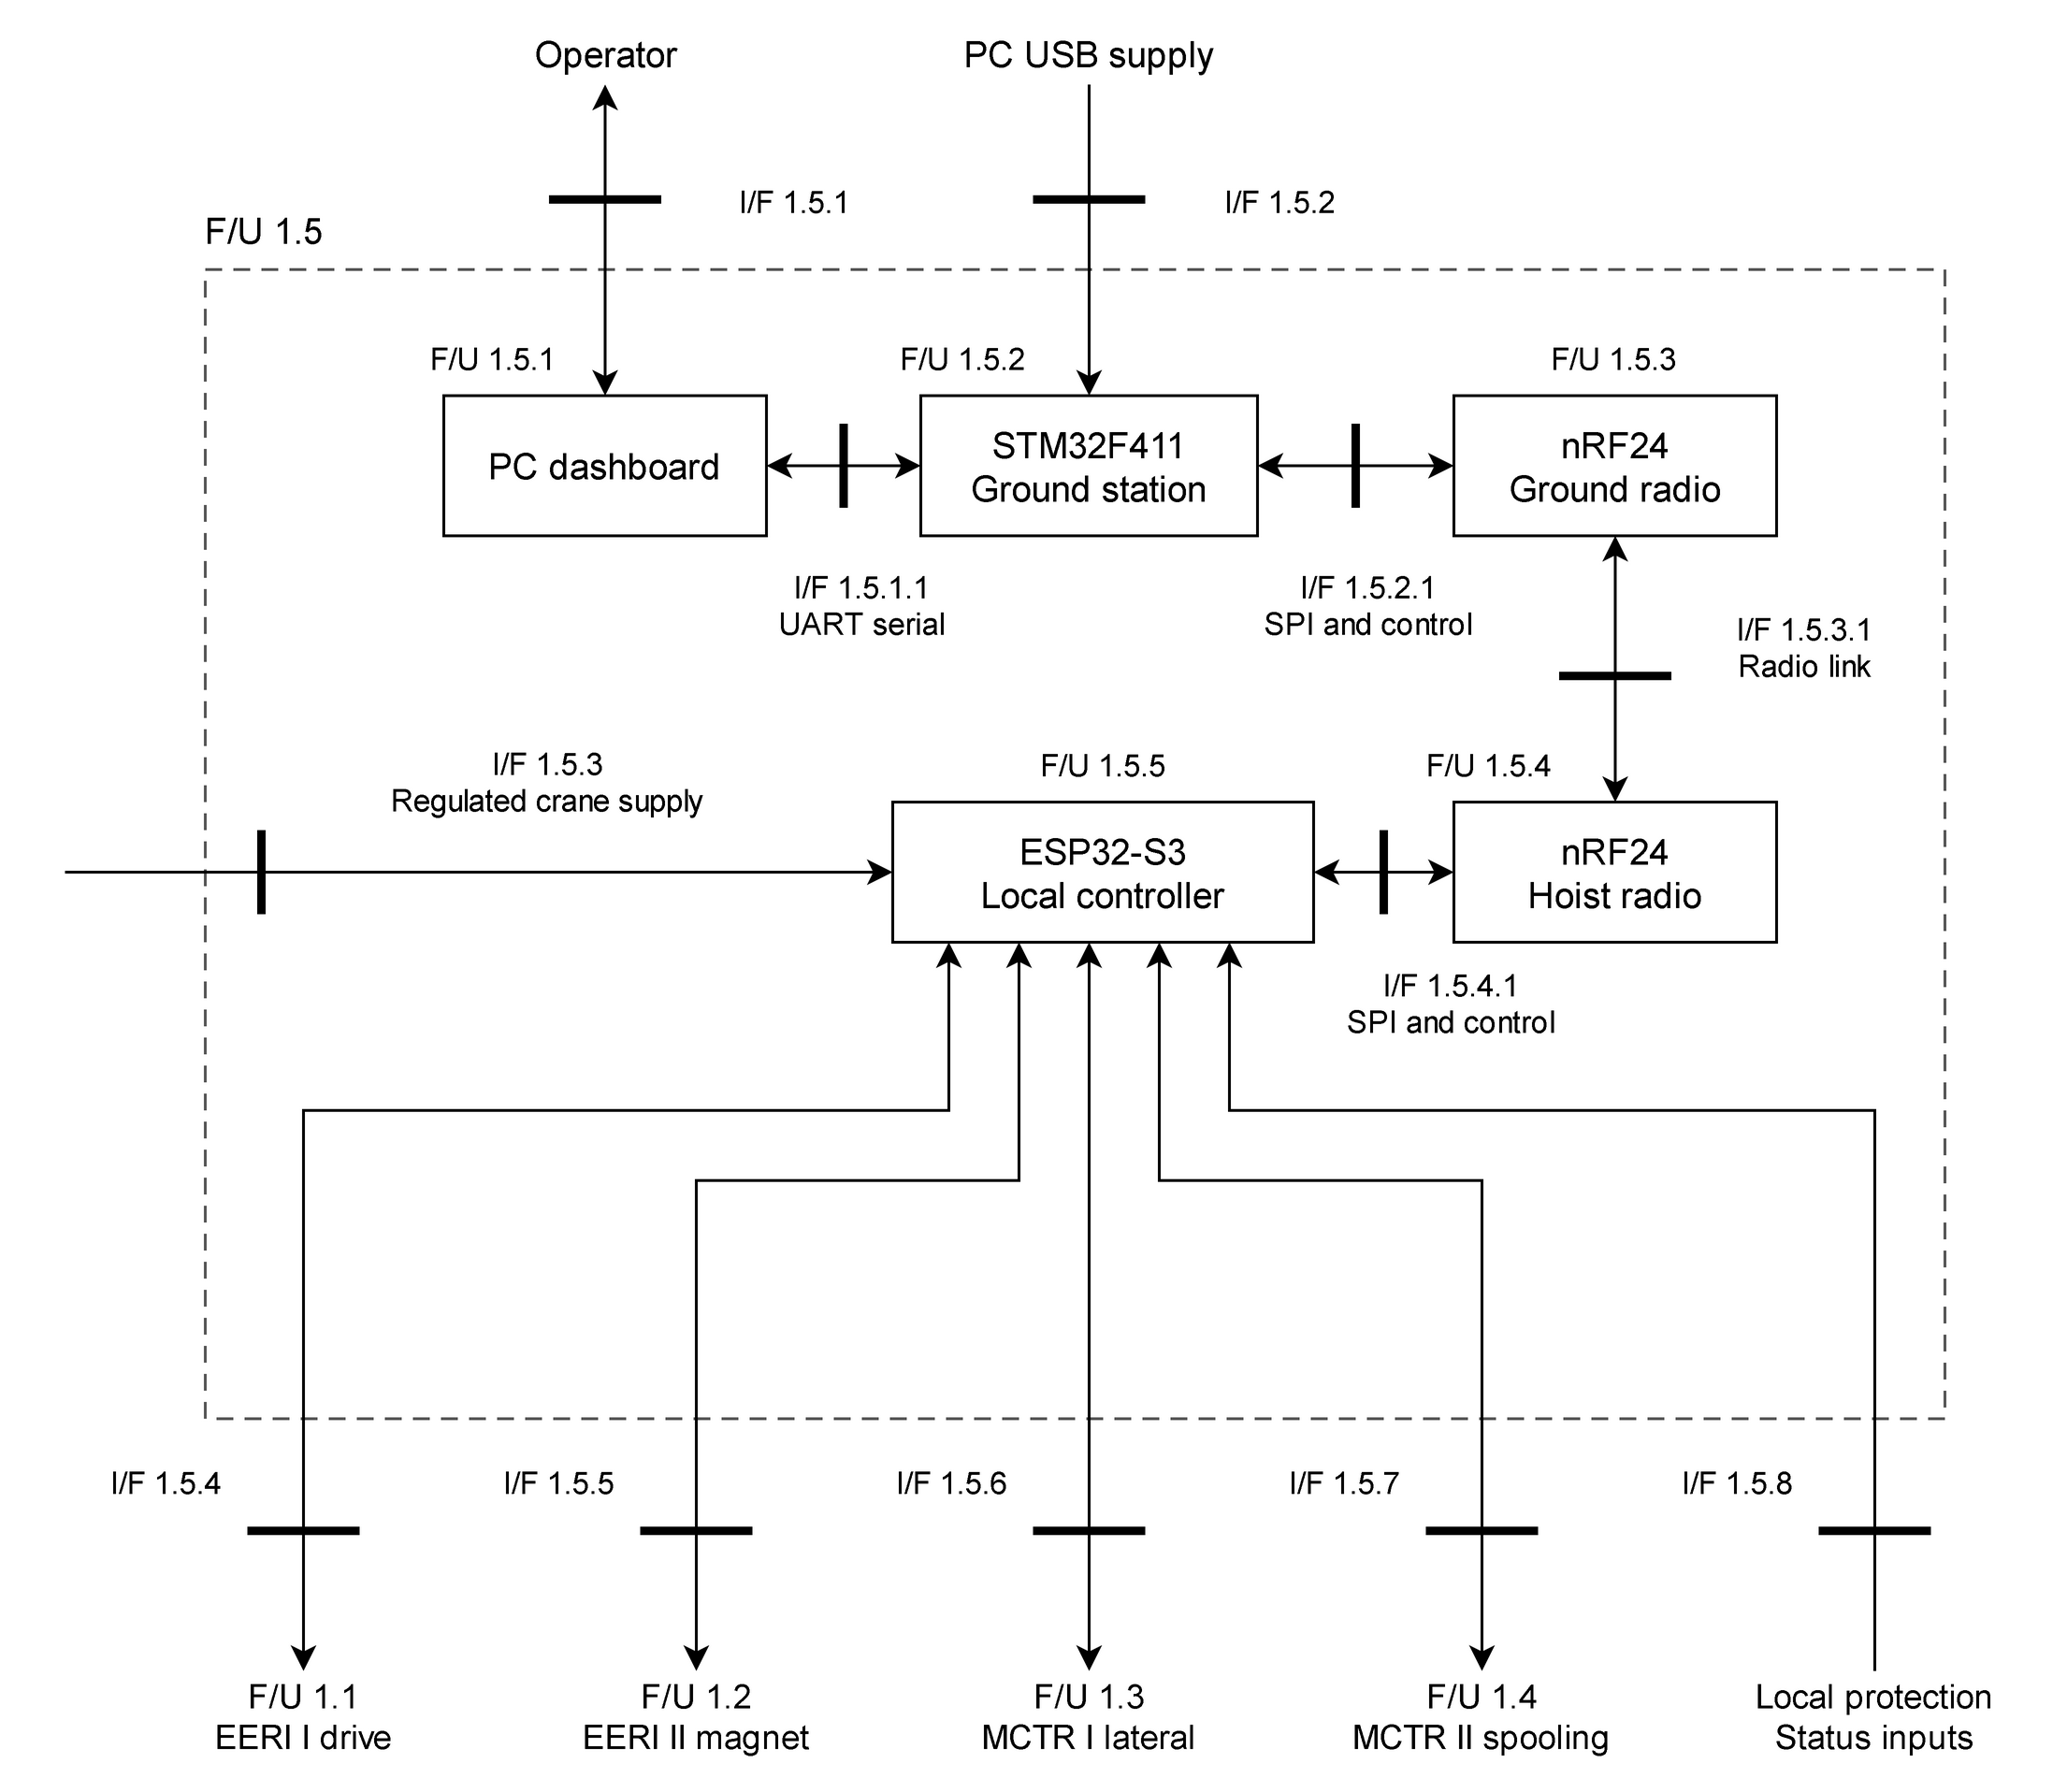
\includegraphics[width=0.85\textwidth]
        {figures/Figure_3_5_System_Architecture.png}
    \caption{Proposed system architecture of REII F/U~1.5.}
    \label{fig:reii-architecture}
\end{figure}

\section{Summary of Interfaces}
\label{sec:summary-of-interfaces}
This section lists each of the interfaces introduced above organised according to their nature, which is either mechanical, electrical, signal, or general. These interfacees are then assigned to each role in chapter \ref{ch:interface-control}.

\subsection{Mechanical Interfaces}
\label{subsec:mechanical-interfaces}
\begin{itemize}
    \item \textbf{EEII I:} I/F 1.8~M connect the 3-phase induction motor to MCTR II (motor shaft to gearbox).
    \item \textbf{MCTR II:} I/F 1.1~M (hoist baseplate to MCTR I mounting plate), I/F 1.3~M (rope to magnetic attachment), I/F 1.8~M (motor shaft to gearbox), and internal I/F \fuMII.1~M (gearbox to drum), \fuMII.3~M (brake to shaft), \fuMII.4~M (rope to load cell).
\end{itemize}

\subsection{Electrical Interfaces}
\label{subsec:electrical-interfaces}
\begin{itemize}
    \item \textbf{EEII I:} I/F 1.0 supplies mains power to the drive electronics subsystem. 
    I/F 1.2 E and I/F 1.6 E supply to the required DC power supplies. I/F 1.7 E provides the 3-phase AC to the
    induction motor.
    \item \textbf{MCTR II:} I/F 1.7~E (motor power from EEII~I) and internal I/F \fuMII.2~E (Brake PSU to brake coil).
\end{itemize}

\subsection{Signal Interfaces}
\label{subsec:signal-interfaces}
\begin{itemize}
    \item \textbf{EEII I:} I/F 1.5 S connects the REII controller to the drive electronics. The controller is
    electrically isolated from the high voltage of the inverter (supplied PWM signbals).
    \item \textbf{MCTR II:} I/F 1.9~S (HX711 to controller), I/F 1.10~S (brake release command) and internal I/F \fuMII.5~S (load cell to HX711).
\end{itemize}

\subsection{General Interfaces}
\label{subsec:general-interfaces}

% ============================================================
%  CHAPTER 4 – INTERFACES
% ============================================================
\chapter{Interface Control}
\label{ch:interface-control}
This chapter describes each of the interfaces introduced in chapter~\ref{ch:system-design}. Each interface listed in section~\ref{sec:summary-of-interfaces}, is described and allocated to a role in section~\ref{sec:work-allocation}.

\section{Work Allocation}
\label{sec:work-allocation}
This section ascribes each interface sa the responsibility of the role under which it is described. Each member read and confirmed their responsibilities and interfaces under their jurisdiction as indicated below. By having their name printed next to their role they have accepted the responsibility and are the liable person for all interfaces listed in their section.

\subsection{EERI I:  }
\label{subsec:eeri1-interfaces}
EERI I Drive Electroncics by Jopie Roux.
\begin{table}[H]
    \centering
    \caption{Operational Interfaces.}
    \label{tab1:interfaces-eeri1}
    \begin{tabular}{@{} l l l p{5cm} @{}}
        \toprule
        \textbf{Interface} & \textbf{From} & \textbf{To} & \textbf{Description} \\
        \midrule
        I1 & F/U 1.0 & F/U 2.0 & Description of data/power/signal. \\
        I/F 1.2 & F/U 2.0 & F/U 3.0 & Description. \\
        I/F 1.2 & F/U 2.0 & F/U 3.0 & Description. \\
        I/F 1.2 & F/U 2.0 & F/U 3.0 & Description. \\
        I/F 1.2 & F/U 2.0 & F/U 3.0 & Description. \\
        I/F 1.2 & F/U 2.0 & F/U 3.0 & Description. \\
        I/F 1.2 & F/U 2.0 & F/U 3.0 & Description. \\
        \bottomrule
    \end{tabular}
\end{table}


\begin{table}[H]
    \centering
    \caption{Operational Interfaces.}
    \label{tab2:interfaces-eeri1}
    \begin{tabular}{@{} l l l p{5cm} @{}}
        \toprule
        \textbf{Interface} & \textbf{From} & \textbf{To} & \textbf{Description} \\
        \midrule
        I1 & F/U 1.0 & F/U 2.0 & Description of data/power/signal. \\
        I/F 1.2 & F/U 2.0 & F/U 3.0 & Description. \\
        I/F 1.2 & F/U 2.0 & F/U 3.0 & Description. \\
        I/F 1.2 & F/U 2.0 & F/U 3.0 & Description. \\
        I/F 1.2 & F/U 2.0 & F/U 3.0 & Description. \\
        I/F 1.2 & F/U 2.0 & F/U 3.0 & Description. \\
        I/F 1.2 & F/U 2.0 & F/U 3.0 & Description. \\
        \bottomrule
    \end{tabular}
\end{table}

\subsection{EERI II: }
\label{subsec:eeri2-interfaces}
EERI II Magnetic Load Attachment by JP Smith.
\begin{table}[H]
    \centering
    \caption{Operational Interfaces.}
    \label{tab:interfaces-eeri2}
    \begin{tabular}{@{} l l l p{5cm} @{}}
        \toprule
        \textbf{Interface} & \textbf{From} & \textbf{To} & \textbf{Description} \\
        \midrule
        I1 & F/U 1.0 & F/U 2.0 & [Description of data/power/signal.] \\
        I2 & F/U 2.0 & F/U 3.0 & [Description.] \\
        \bottomrule
    \end{tabular}
\end{table}



\subsection{MCTR I: }
\label{subsec:mctr1-interfaces}
MCTR I Lateral Movement by Romeo Mapasa.
\begin{table}[H]
    \centering
    \caption{Operational Interfaces.}
    \label{tab:interfaces-mctr1}
    \begin{tabular}{@{} l l l p{5cm} @{}}
        \toprule
        \textbf{Interface} & \textbf{From} & \textbf{To} & \textbf{Description} \\
        \midrule
        I1 & F/U 1.0 & F/U 2.0 & [Description of data/power/signal.] \\
        I2 & F/U 2.0 & F/U 3.0 & [Description.] \\
        \bottomrule
    \end{tabular}
\end{table}




\subsection{MCTR II: Juan Fourie}
\label{subsec:mctr2-interfaces}
MCTR II Spooling by Juan Fourie.
% =====================================================================
%  mctr2_parameters.tex  --  MCTR II (Spooling) parameter + calculation sheet
%
%  HOW TO USE
%   * Edit ONLY the \In... values in Section 1. Everything in Section 2
%     (\Raw... results) is computed from them by \fpeval, so every
%     table, equation and sentence that quotes a result updates on the
%     next compile.
%   * Units are noted per line. Torques in N.m unless stated.
%   * Display helpers:  \shown{Name}{digits}        -> number only
%                       \showv{Name}{digits}{unit}  -> number + unit
%   * This file is safe to \input from several chapters (loads once).
%   * Needs: LaTeX >= 2021 (\fpeval in kernel), amsmath, xcolor.
% =====================================================================
\ifdefined\MCTRIIparamsloaded\else
\def\MCTRIIparamsloaded{}

\providecommand{\tbd}[1]{\textcolor{red}{\textbf{[TBD: #1]}}}
\newcommand{\val}[2]{\ensuremath{#1\,\mathrm{#2}}}
\newcommand{\shown}[2]{\fpeval{round(\csname Raw#1\endcsname,#2)}}
\newcommand{\showv}[3]{\val{\fpeval{round(\csname Raw#1\endcsname,#2)}}{#3}}
% PASS/FAIL helpers: \passge{value}{limit} passes when value >= limit
\newcommand{\passge}[2]{\ifdim #1pt<#2pt \textcolor{red}{\textbf{FAIL}}\else\textcolor{green!45!black}{\textbf{PASS}}\fi}
\newcommand{\passle}[2]{\ifdim #1pt>#2pt \textcolor{red}{\textbf{FAIL}}\else\textcolor{green!45!black}{\textbf{PASS}}\fi}

% Functional-unit number of MCTR II (Level 1 drawing: F/U 1.4).
% NOTE: the Level 2 drawing currently labels sub-units 1.3.x; change the
% drawing to 1.4.x (or set this to 1.3 to match the drawing, but 1.3 is MCTR I).
\newcommand{\fuMII}{1.3}

% ---------------------------------------------------------------------
% 1. INPUTS  (edit these)
% ---------------------------------------------------------------------
% -- Loads, stroke, timing
\newcommand{\InMassRated}{20}    % kg   rated payload (PHY1)
\newcommand{\InMassDesign}{30}   % kg   design overload case (analysis only)
\newcommand{\InMassAttach}{2}    % kg   magnet + hook hanging on rope  [TBD: weigh]
\newcommand{\InGrav}{9.81}       % m/s^2
\newcommand{\InStroke}{1.6}      % m     hoist stroke (PT2)
\newcommand{\InTimeReq}{20}      % s     max stroke time (PT2)
\newcommand{\InServiceF}{1.5}    % -     service factor on drum torque
\newcommand{\InSFreq}{1.5}       % -     minimum acceptable safety factor (strength checks)
% -- Drum and rope
\newcommand{\InDrumD}{50}        % mm    drum core diameter (FROZEN; 70 mm entry removed)
\newcommand{\InDrumH}{60}        % mm    drum usable length
\newcommand{\InRopeD}{5}         % mm    rope diameter
\newcommand{\InRopeCentre}{1}    % 1 = tension acts at rope centre-line (D+d); 0 = old spreadsheet (D only)
% -- Motor and VSD
\newcommand{\InMotorP}{180}      % W     Askari MS632-4
\newcommand{\InMotorN}{1360}     % rpm   at rated frequency
\newcommand{\InMotorF}{50}       % Hz    rated frequency
\newcommand{\InVsdF}{50}         % Hz    frequency VSD will actually deliver  [TBD: EEII I to confirm]
% -- Gearbox (stage A = motor side, stage B = drum side)
\newcommand{\InNpA}{16}   \newcommand{\InNgA}{102}   % pinion / gear teeth, stage A
\newcommand{\InNpB}{16}   \newcommand{\InNgB}{102}   % pinion / gear teeth, stage B
\newcommand{\InModA}{1.5} \newcommand{\InModB}{2}    % mm module
\newcommand{\InFwA}{10}   \newcommand{\InFwB}{15}    % mm face width
\newcommand{\InPhi}{25}          % deg   pressure angle (use 24 if Inventor forces it; both gears of a mesh must match)
\newcommand{\InYpA}{0.296}       % Lewis form factor, pinion  (Shigley Tbl 14-2, 20 deg value: conservative for 25 deg)
\newcommand{\InYgA}{0.447}       % Lewis form factor, gear
\newcommand{\InYpB}{0.296}
\newcommand{\InYgB}{0.447}
\newcommand{\InEta}{0.95}        % -     efficiency per gear stage
\newcommand{\InSigAllow}{20}     % MPa   allowable PETG root stress [GUESS: replace with printed-coupon result / SF]
\newcommand{\InClear}{0.25}      % mm    added centre-distance clearance (printed backlash)
\newcommand{\InBed}{220}         % mm    print bed edge length [TBD: confirm printer]
% -- Shaft, hub and fastener
\newcommand{\InShaftD}{10}       % mm    shaft diameter
\newcommand{\InSpan}{100}        % mm    bearing span (centre-to-centre)
\newcommand{\InKt}{2}            % -     bending stress-concentration factor, cross-hole
\newcommand{\InKts}{2}           % -     torsion stress-concentration factor, cross-hole
\newcommand{\InSy}{250}          % MPa   yield strength  [TBD: replace with certified grade, e.g. EN8 bright bar]
\newcommand{\InBoltD}{4}         % mm    cross-bolt diameter
\newcommand{\InHubWall}{8}       % mm    hub wall length bearing on bolt
\newcommand{\InHubAllow}{20}     % MPa   allowable PETG bearing stress [GUESS]
% -- Brake
\newcommand{\InBrakeSF}{2}       % -     brake torque safety factor
\newcommand{\InBrakeRated}{0}    % N.m   datasheet holding torque; 0 = not yet known  [TBD: datasheet]
% -- Load cell and HX711
\newcommand{\InCellCap}{100}     % kg    YZC-516 rated capacity
\newcommand{\InCellSens}{2}      % mV/V  rated output [TBD: datasheet]
\newcommand{\InExc}{5}           % V     excitation (HX711 supply)
\newcommand{\InGain}{128}        % -     HX711 channel A gain
\newcommand{\InSps}{80}          % SPS   HX711 output rate (RATE pin high)
\newcommand{\InFilt}{4}          % -     samples averaged by interlock filter
\newcommand{\InNoise}{500}       % counts peak-to-peak noise [GUESS: measure with motor running]
\newcommand{\InTrip}{1.25}       % -     overload trip as multiple of (rated + attachment)
% -- Cost (R, incl. VAT and shipping, from Cost_and_Budget.xlsx)
\newcommand{\InBudget}{5000}
\newcommand{\InCostBearings}{116.24}
\newcommand{\InCostCell}{429.00}     % [CHECK: sheet unit 493.35 + 135.70 shipping = 629.05]
\newcommand{\InCostHX}{179.40}       % [CHECK: unit price 43.70]
\newcommand{\InCostPSU}{390.17}
\newcommand{\InCostBrake}{907.68}    % excluded from the sheet's own subtotal

% ---------------------------------------------------------------------
% 2. DERIVED RESULTS  (do not edit)
% ---------------------------------------------------------------------
% -- Kinematics
\newcommand{\RawDeff}{\fpeval{\InDrumD+\InRopeCentre*\InRopeD}}
\newcommand{\RawVreq}{\fpeval{\InStroke*1000/\InTimeReq}}
\newcommand{\RawWraps}{\fpeval{\InStroke*1000/(pi*\RawDeff)}}
\newcommand{\RawWrapsFit}{\fpeval{floor(\InDrumH/\InRopeD)}}
\newcommand{\RawiA}{\fpeval{\InNgA/\InNpA}}
\newcommand{\RawiB}{\fpeval{\InNgB/\InNpB}}
\newcommand{\RawiT}{\fpeval{\RawiA*\RawiB}}
\newcommand{\RawNmot}{\fpeval{\InMotorN*\InVsdF/\InMotorF}}
\newcommand{\RawNdrum}{\fpeval{\RawNmot/\RawiT}}
\newcommand{\RawVline}{\fpeval{pi*\RawDeff*\RawNdrum/60}}
\newcommand{\RawTstroke}{\fpeval{\InStroke*1000/\RawVline}}
\newcommand{\RawSpeedMargin}{\fpeval{(\RawVline/\RawVreq-1)*100}}
\newcommand{\RawiReq}{\fpeval{pi*\RawDeff*\RawNmot/(60*\RawVreq)}}
\newcommand{\RawFmin}{\fpeval{\RawVreq*60*\RawiT/(pi*\RawDeff)*\InMotorF/\InMotorN}}
% -- Drum torque, motor sizing
\newcommand{\RawFropeR}{\fpeval{\InMassRated*\InGrav}}
\newcommand{\RawFropeD}{\fpeval{\InMassDesign*\InGrav}}
\newcommand{\RawTdrR}{\fpeval{\InMassRated*\InGrav*\RawDeff/2000}}
\newcommand{\RawTdrD}{\fpeval{\InMassDesign*\InGrav*\RawDeff/2000*\InServiceF}}
\newcommand{\RawTdrSheet}{\fpeval{\InMassDesign*\InGrav*\InDrumD/2000*\InServiceF}}
\newcommand{\RawEtaGB}{\fpeval{\InEta*\InEta}}
\newcommand{\RawTmReq}{\fpeval{\RawTdrR/(\RawiT*\RawEtaGB)}}
\newcommand{\RawTmRated}{\fpeval{\InMotorP/(2*pi*\InMotorN/60)}}
\newcommand{\RawTmMargin}{\fpeval{\RawTmRated/\RawTmReq}}
\newcommand{\RawPmech}{\fpeval{\InMassRated*\InGrav*\RawVline/1000/\RawEtaGB}}
\newcommand{\RawPavail}{\fpeval{\InMotorP*\InVsdF/\InMotorF}}
% -- Gear loads (design case) and Lewis stress
\newcommand{\RawTtwo}{\fpeval{\RawTdrD/(\RawiB*\InEta)}}
\newcommand{\RawTone}{\fpeval{\RawTtwo/(\RawiA*\InEta)}}
\newcommand{\RawFtB}{\fpeval{2*\RawTtwo*1000/(\InModB*\InNpB)}}
\newcommand{\RawFtA}{\fpeval{2*\RawTone*1000/(\InModA*\InNpA)}}
\newcommand{\RawFnB}{\fpeval{\RawFtB/cosd(\InPhi)}}
\newcommand{\RawFnA}{\fpeval{\RawFtA/cosd(\InPhi)}}
\newcommand{\RawFrB}{\fpeval{\RawFtB*tand(\InPhi)}}
\newcommand{\RawSigPA}{\fpeval{\RawFtA/(\InFwA*\InModA*\InYpA)}}
\newcommand{\RawSigGA}{\fpeval{\RawFtA/(\InFwA*\InModA*\InYgA)}}
\newcommand{\RawSigPB}{\fpeval{\RawFtB/(\InFwB*\InModB*\InYpB)}}
\newcommand{\RawSigGB}{\fpeval{\RawFtB/(\InFwB*\InModB*\InYgB)}}
\newcommand{\RawSFpA}{\fpeval{\InSigAllow/\RawSigPA}}
\newcommand{\RawSFpB}{\fpeval{\InSigAllow/\RawSigPB}}
% -- Gear geometry
\newcommand{\RawDpinA}{\fpeval{\InModA*\InNpA}}
\newcommand{\RawDgearA}{\fpeval{\InModA*\InNgA}}
\newcommand{\RawDpinB}{\fpeval{\InModB*\InNpB}}
\newcommand{\RawDgearB}{\fpeval{\InModB*\InNgB}}
\newcommand{\RawDoGearA}{\fpeval{\InModA*(\InNgA+2)}}
\newcommand{\RawDoGearB}{\fpeval{\InModB*(\InNgB+2)}}
\newcommand{\RawCdA}{\fpeval{\InModA*(\InNpA+\InNgA)/2+\InClear}}
\newcommand{\RawCdB}{\fpeval{\InModB*(\InNpB+\InNgB)/2+\InClear}}
\newcommand{\RawZmin}{\fpeval{2/(sind(\InPhi)^2)}}
\newcommand{\RawDbPinB}{\fpeval{\RawDpinB*cosd(\InPhi)}}
\newcommand{\RawBedUse}{\fpeval{max(\RawDoGearA,\RawDoGearB)/\InBed*100}}
% -- Shaft (macros with arguments: #1 = payload mass kg, #2 = torque factor)
\newcommand{\Tdr}[2]{\fpeval{#1*\InGrav*\RawDeff/2*#2}}                                   % N.mm
\newcommand{\FgB}[2]{\fpeval{2*\Tdr{#1}{#2}/(\InEta*\InModB*\InNgB*cosd(\InPhi))}}        % N
\newcommand{\Msh}[2]{\fpeval{(#1*\InGrav+\FgB{#1}{#2})*\InSpan/4}}                        % N.mm
\newcommand{\SigBsh}[2]{\fpeval{32*\Msh{#1}{#2}/(pi*\InShaftD^3)}}                        % MPa
\newcommand{\Taush}[2]{\fpeval{16*\Tdr{#1}{#2}/(pi*\InShaftD^3)}}                         % MPa
\newcommand{\VMsh}[2]{\fpeval{sqrt((\InKt*\SigBsh{#1}{#2})^2+3*(\InKts*\Taush{#1}{#2})^2)}} % MPa
\newcommand{\RawFgD}{\FgB{\InMassDesign}{\InServiceF}}
\newcommand{\RawMshD}{\Msh{\InMassDesign}{\InServiceF}}
\newcommand{\RawSigBD}{\SigBsh{\InMassDesign}{\InServiceF}}
\newcommand{\RawTauD}{\Taush{\InMassDesign}{\InServiceF}}
\newcommand{\RawVMD}{\VMsh{\InMassDesign}{\InServiceF}}
\newcommand{\RawVMR}{\VMsh{\InMassRated}{1}}
\newcommand{\RawSFsD}{\fpeval{\InSy/\RawVMD}}
\newcommand{\RawSFsR}{\fpeval{\InSy/\RawVMR}}
% -- Hub / cross-bolt (design case, drum shaft)
\newcommand{\RawFside}{\fpeval{\RawTdrD*1000/\InShaftD}}
\newcommand{\RawSigHub}{\fpeval{\RawFside/(\InBoltD*\InHubWall)}}
\newcommand{\RawTauBolt}{\fpeval{\RawFside/(pi*\InBoltD^2/4)}}
\newcommand{\RawSFhub}{\fpeval{\InHubAllow/\RawSigHub}}
% -- Rated-case (20 kg, no service factor) checks for gears and hub
\newcommand{\RawLoadRatio}{\fpeval{\RawTdrR/\RawTdrD}}
\newcommand{\RawSFpAR}{\fpeval{\RawSFpA/\RawLoadRatio}}
\newcommand{\RawSFpBR}{\fpeval{\RawSFpB/\RawLoadRatio}}
\newcommand{\RawSigHubR}{\fpeval{\RawSigHub*\RawLoadRatio}}
\newcommand{\RawSFhubR}{\fpeval{\InHubAllow/\RawSigHubR}}
% -- Brake
\newcommand{\RawTholdDrum}{\fpeval{\InMassDesign*\InGrav*\RawDeff/2000}}
\newcommand{\RawTholdIn}{\fpeval{\RawTholdDrum/\RawiT}}
\newcommand{\RawBrakeReqDrum}{\fpeval{\RawTholdDrum*\InBrakeSF}}
\newcommand{\RawBrakeReqIn}{\fpeval{\RawTholdIn*\InBrakeSF}}
\newcommand{\BrakeMarginIn}{\ifdim\InBrakeRated pt=0pt\tbd{datasheet torque}\else\fpeval{round(\InBrakeRated/\RawBrakeReqIn,1)}\fi}
\newcommand{\BrakeMarginDrum}{\ifdim\InBrakeRated pt=0pt\tbd{datasheet torque}\else\fpeval{round(\InBrakeRated/\RawBrakeReqDrum,1)}\fi}
% -- Load cell and HX711
\newcommand{\RawFcell}{\fpeval{(\InMassRated+\InMassAttach)*\InGrav}}
\newcommand{\RawMtrip}{\fpeval{(\InMassRated+\InMassAttach)*\InTrip}}
\newcommand{\RawCellUse}{\fpeval{\RawMtrip/\InCellCap*100}}
\newcommand{\RawSigFS}{\fpeval{\InCellSens*\InExc}}
\newcommand{\RawAdcRange}{\fpeval{0.5*\InExc/\InGain*1000}}
\newcommand{\RawCntPerKg}{\fpeval{\InCellSens/1000/\InCellCap*\InGain/0.5*2^23}}
\newcommand{\RawResG}{\fpeval{\InNoise/\RawCntPerKg*1000}}
\newcommand{\RawLatency}{\fpeval{\InFilt/\InSps*1000}}
\newcommand{\RawTravel}{\fpeval{\RawVline*\RawLatency/1000}}
% -- Cost
\newcommand{\RawCostTot}{\fpeval{\InCostBearings+\InCostCell+\InCostHX+\InCostPSU+\InCostBrake}}
\newcommand{\RawBudgetLeft}{\fpeval{\InBudget-\RawCostTot}}
\newcommand{\RawBudgetUse}{\fpeval{\RawCostTot/\InBudget*100}}
\fi


% ---- INSERTED FROM DRAWINGS: Level 1 and Level 2 (MCTR II) -------------
Tables~\ref{tab:interfaces-mctr2} and~\ref{tab:interfaces-mctr2-internal} list every interface that crosses the
MCTR II boundary (Level 1 numbering) and every interface between its internal
functional units (Level 2 numbering). The type letter follows the drawing:
M = mechanical, E = electrical, S = signal. Entries marked
\textcolor{red}{TBD} were inferred from the drawing labels and must be
confirmed by the owner of the other party before sign-off.
 
\begin{table}[H]
    \centering
    \caption{External interfaces of MCTR II (F/U \fuMII, Level 1).}
    \label{tab:interfaces-mctr2}
    \footnotesize
    \renewcommand{\arraystretch}{1.25}
    \begin{tabularx}{\textwidth}{@{} l p{2.6cm} p{1.6cm} X @{}}
        \toprule
        \textbf{Interface} & \textbf{From} & \textbf{To} & \textbf{Description and key parameters} \\
        \midrule
        I/F 1.1 M & F/U 1.3 (mounting plate) & F/U \fuMII &
            Bolted mounting of the hoist baseplate (6061-T6, \tbd{mm}) on the
            MCTR I mounting plate. Plate carries the rope reaction of
            \showv{FropeD}{0}{N} (design case). Hole pattern \tbd{}.
            \tbd{confirm against drawing} \\
        I/F 1.3 M & F/U \fuMII.4 (rope) & F/U 1.2 &
            Rope termination to the magnetic load attachment. Rated payload
            \InMassRated\,kg plus attachment \InMassAttach\,kg.
            \tbd{confirm against drawing} \\
        I/F 1.7 E & F/U 1.1 & F/U \fuMII &
            3-phase power to the induction motor from the VSD
            (\InMotorP\,W, \InMotorN\,rpm at \InMotorF\,Hz). Delivered
            frequency \tbd{Hz}. Mains feed to the Brake PSU
            \tbd{not shown in drawing: add interface or confirm it is part
            of I/F 1.7 E}. \\
        I/F 1.8 M & F/U 1.1 (motor) & F/U \fuMII.1 &
            Motor shaft (11\,mm, $4\times16$\,mm keyway) to gearbox input
            shaft (\InShaftD\,mm) through a flexible coupling and a separate
            input stub shaft on its own bearings. Coupling \tbd{part no.}. \\
        I/F 1.9 S & F/U \fuMII.6 & F/U 1.5 &
            HX711 digital output (DOUT/SCK), 24-bit, \InSps\,SPS, logic level
            \tbd{3.3/5\,V}. Load reading used for telemetry and interlock. \\
        I/F 1.10 S & F/U 1.5 & F/U \fuMII.3 &
            Brake release command via relay. Active-high releases; the
            default (reset, watchdog, power loss) is brake engaged, in
            hardware. \\
        \bottomrule
    \end{tabularx}
\end{table}
 
\begin{table}[H]
    \centering
    \caption{Internal interfaces of MCTR II (F/U \fuMII, Level 2).}
    \label{tab:interfaces-mctr2-internal}
    \footnotesize
    \renewcommand{\arraystretch}{1.25}
    \begin{tabularx}{\textwidth}{@{} l p{2.6cm} p{1.6cm} X @{}}
        \toprule
        \textbf{Interface} & \textbf{From} & \textbf{To} & \textbf{Description and key parameters} \\
        \midrule
        I/F \fuMII.1 M & F/U \fuMII.1 & F/U \fuMII.4 &
            Gearbox output shaft to drum hub; M4 cross-bolt through a reamed
            hole. Design torque \showv{TdrD}{1}{N\,m} (\InMassDesign\,kg
            overload with service factor \InServiceF). \\
        I/F \fuMII.2 E & F/U \fuMII.2 & F/U \fuMII.3 &
            48\,V DC supply to the brake coil through a relay, with
            flyback suppression. Coil current \tbd{A}. \\
        I/F \fuMII.3 M & F/U \fuMII.3 & F/U \fuMII.1 &
            Brake on the gearbox input stub shaft (provisional;
            drum shaft is the alternative). Required rating
            \showv{BrakeReqIn}{2}{N\,m} (input shaft) or
            \showv{BrakeReqDrum}{1}{N\,m} (drum shaft), safety factor
            \InBrakeSF. \\
        I/F \fuMII.4 M & F/U \fuMII.4 & F/U \fuMII.5 &
            Rope over a sheave suspended from the load cell. Vertical load
            \showv{Fcell}{0}{N} at rated payload; equal side load on the
            cell from the horizontal rope leg. \\
        I/F \fuMII.5 S & F/U \fuMII.5 & F/U \fuMII.6 &
            4-wire bridge signal, \InCellSens\,mV/V rated output, shielded
            cable, full-scale \showv{SigFS}{1}{mV} against an ADC range of
            \showv{AdcRange}{1}{mV}. \\
        \bottomrule
    \end{tabularx}
\end{table}
 
\noindent\textbf{Open interface questions raised by this table:}
(i) the mains supply to the Brake PSU, required by the system specification to be
distributed by EEII~I, does not appear on the drawings; (ii) the power and
current-sense cable of the magnetic attachment must follow the rope without
carrying tension, which is a cable interface between MCTR II and EEII~II that
is also not drawn; (iii) the drawing numbers the MCTR II sub-units 1.3.x,
which duplicates MCTR I (F/U 1.3), so they are renumbered 1.4.x here.



\subsection{REII: Anton Swanepoel}
\label{subsec:reii-interfaces}
REII Remote Control Dashboard by Anton Swanepoel.

Tables~\ref{tab:reii-external} and~\ref{tab:reii-internal}
define the proposed external and internal interfaces in Figure~3.5.
TBD parameters require agreement.
\cite{nwu_sysrs2026,nwu_reii_scope2026}

\begingroup
\setlength{\tabcolsep}{4pt}
\renewcommand{\arraystretch}{1.15}



\begin{table}[H]
    \centering
    \footnotesize
    \caption{External interfaces of REII (F/U 1.5, Level 1).}
    \label{tab:reii-external}

    \begin{tabularx}{\textwidth}{@{}
        >{\raggedright\arraybackslash}p{2.15cm}
        >{\raggedright\arraybackslash}p{2.7cm}
        >{\raggedright\arraybackslash}p{2.9cm}
        >{\raggedright\arraybackslash}X
    @{}}
        \toprule
        \textbf{Interface} &
        \textbf{From} &
        \textbf{To} &
        \textbf{Description and key parameters} \\
        \midrule

        Operator link\newline (1.5.1) &
        Operator &
        Python dashboard\newline (F/U 1.5.1) &
        Operator commands enter; displayed telemetry and faults return.
        \\[3pt]

        Ground supply\newline (1.5.2) &
        PC supply &
        Ground station and radio\newline (F/U 1.5.2, 1.5.3) &
        PC USB power supplies the UART-connected ground station;
        its radio uses regulated 3.3~V.
        \\[3pt]

        Crane supply\newline (1.5.3) &
        Crane supply &
        Controller and hoist radio\newline (F/U 1.5.5, 1.5.4) &
        Regulated 5~V would feed the S3 board; its 3.3~V
        peripheral rail would supply the radio.
        \\[3pt]

        Inverter control\newline (1.5.4) &
        ESP32-S3 controller\newline (F/U 1.5.5) &
        Drive electronics\newline (F/U 1.1) &
        Six isolated PWM paths plus reserve; current feedback
        below 2.048~V for fault inference.
        \textcolor{red}{[TBD: PWM timing and active levels.]}
        \\[3pt]

        Magnet control\newline (1.5.5) &
        ESP32-S3 controller\newline (F/U 1.5.5) &
        Magnetic attachment\newline (F/U 1.2) &
        Isolated magnet PWM; current feedback below 2.048~V
        for investigating an on-load indicator.
        \textcolor{red}{[TBD: current-signature discrimination,
        calibration and load-support criterion.]}
        \\[3pt]

        Lateral control\newline (1.5.6) &
        ESP32-S3 controller\newline (F/U 1.5.5) &
        Lateral movement\newline (F/U 1.3) &
        PWM and direction commands; quadrature encoder feedback
        for lateral position and speed.
        \textcolor{red}{[TBD: encoder scale and polarity.]}
        \\[3pt]

        Spooling interface\newline (1.5.7) &
        ESP32-S3 controller\newline (F/U 1.5.5) &
        Spooling subsystem\newline (F/U 1.4) &
        REII would power the HX711 (3.3~V/GND), drive SCK
        and read DAT. The proposed optocoupler brake command
        is HIGH to release and LOW to hold; loss of brake
        power would engage the brake. Group links:
        I/F~1.9 load and I/F~1.10 brake.
        \textcolor{red}{[TBD: load calibration and final brake polarity.]}
        \\[3pt]

        Protection status\newline (1.5.8) &
        Local protection &
        ESP32-S3 controller\newline (F/U 1.5.5) &
        The hardware E-stop would remove power from the drive
        electronics independently of software (PHY2).A proposed status signal
        would inform the ESP32-S3 when the E-stop is activated.
        \textcolor{red}{[TBD: E-stop wiring, status signal and
        integration testing.]}
        \\

        \bottomrule
    \end{tabularx}
\end{table}



\begin{table}[H]
    \centering
    \footnotesize
    \caption{Internal interfaces of REII (F/U 1.5, Level 2).}
    \label{tab:reii-internal}

    \begin{tabularx}{\textwidth}{@{}
        >{\raggedright\arraybackslash}p{2.15cm}
        >{\raggedright\arraybackslash}p{2.7cm}
        >{\raggedright\arraybackslash}p{2.9cm}
        >{\raggedright\arraybackslash}X
    @{}}
        \toprule
        \textbf{Interface} &
        \textbf{From} &
        \textbf{To} &
        \textbf{Description and key parameters} \\
        \midrule

        PC serial link\newline (1.5.1.1) &
        Python dashboard\newline (F/U 1.5.1) &
        STM32 ground station\newline (F/U 1.5.2) &
        UART serial requests; replies and diagnostics return
        at 115200~bit/s, 8N1.
        \\[3pt]

        Ground radio SPI\newline (1.5.2.1) &
        STM32 ground station\newline (F/U 1.5.2) &
        Ground radio\newline (F/U 1.5.3) &
        SPI and radio-control signals; received frames and
        radio status return.
        \\[3pt]

        Wireless link\newline (1.5.3.1) &
        Ground radio\newline (F/U 1.5.3) &
        Hoist radio\newline (F/U 1.5.4) &
        Bidirectional nRF24 link carrying commands, results
        and operational telemetry.
        \\[3pt]

        Hoist radio SPI\newline (1.5.4.1) &
        Hoist radio\newline (F/U 1.5.4) &
        ESP32-S3 controller\newline (F/U 1.5.5) &
        Received commands pass to the controller; SPI control
        and reply data return.
        \\

        \bottomrule
    \end{tabularx}
\end{table}

\endgroup

\noindent
Controller logic operates at 3.3~V.
\cite{nwu_s3_board2026}





% ============================================================
%  CHAPTER 5 – Main Design Decisions
% ============================================================
\chapter{Design Decisions}
\label{ch:design-decisions}
This chapter discusses each of the major design decisions that have been made by each of the listed roles relative to their responsibilites. This chapter also discusses the alternatives to the chosen solutions and the reasons for the decisions made.

\section{EERI I:Subsystem: Drive Electronics}
\label{sec:eeri1-subsystem-drive-electronics}

The main power-electronic components were selected according to voltage and current requirments and switching
performance, thermal capacity compatibility with control circuitry and cost. Preference was given to components
that proivided sufficienty fault and trtansient headroom without exceeding the budget. The selected components 
were subsequently used during the low voltage test of the drive ciruitry.

\subsection{Bridge Rectifier}

In Table \ref{tab:eeri1-rectifiers} below the available bridge rectifiers for EEII are compared. 

\begin{table}[H]
    \centering
    \caption{Available bridge rectifiers for EEII I.}
    \label{tab:eeri1-rectifiers}

    \begin{tabular}{@{} l c c c c c @{}}
        \toprule
        \textbf{Component} &
        \shortstack{\textbf{Reverse Voltage}\\\textbf{Rating}} &
        \shortstack{\textbf{Average Current}\\\textbf{Rating}} &
        \shortstack{\textbf{Surge}\\\textbf{Current}} &
        \shortstack{\textbf{Thermal}\\\textbf{Resistance}} &
        \textbf{Selected} \\
        \midrule

        GBK25M & 1000 V & 25 A & 350 A & 0.6 $^\circ$C/W & \\

        GBJ1510 & 1000 V & 15 A & 240 A & 0.8 $^\circ$C/W & \checkmark \\

        \bottomrule
    \end{tabular}
\end{table}

Both rectifiers in Table \ref{tab:eeri1-rectifiers} provide a 1000V reverse-voltage rating, which gives a large margin above the 325VDC which 
is obtained from rectify in the 230VAC mains. The GBK25M porvides a higher 25A average current rating and 
350A surge current rating, whereas the GBJ1510 provides a 15A average and 240A surege current rating.

The GJB1510 was selected because its 15A average currnet rating is already well above the nominal current 
rating of the 180 W motor. The extra current capability of the GBK25M would therefore provide no additional
benefit during normal operation. The GBJ1510 still provides the necessary 1000V blocking capacity and 240A 
surge current rating is suffiecient for the application. The datasheet specifies that the rectifier current 
rating should be derated by 20 \% when supplying a capacitive load such as the bulk capacitor. Even after
derating the current capability remains well above the expected operating requirement. 

\subsection{IGBT Selection}

In Table \ref{tab:eeri1-igbt-options} below the available IGBTs for EEII are compared. 

\begin{table}[H]
    \centering
    \caption{Available IGBT options for EEII I.}
    \label{tab:eeri1-igbt-options}

    \small
    \begin{tabular}{@{} l c c c c c c @{}}
        \toprule
        \textbf{Component} &
        \shortstack{\textbf{Voltage}\\\textbf{Rating}} &
        \shortstack{\textbf{Current Rating}\\\textbf{@ 100$^\circ$C}} &
        \shortstack{\textbf{Pulsed}\\\textbf{Current}} &
        \shortstack{\textbf{Thermal}\\\textbf{Resistance}} &
        \shortstack{\textbf{Total Gate}\\\textbf{Charge}} &
        \textbf{Selected} \\
        \midrule

        STGP7NC60HD & 600 V & 14 A & 50 A & 1.56 $^\circ$C/W & 35 nC & \\

        FGH75T65SHDT & 650 V & 75 A & 225 A & 0.33 $^\circ$C/W & 123 nC & \checkmark \\

        \bottomrule
    \end{tabular}
\end{table}

Both devices in Table \ref{tab:eeri1-igbt-options} are suitable for the inverter application and provide voltage ratings well above the  nominal DC
bus voltage.The STGP7NC60HD is rated for 600V and 14A at a case temperature of 100$^\circ$C, with a pulsed current
rating of 50A. The FGH75T65SHDT increases these ratings to 650V and 75A at 100$^\circ$C and 225A pulsed current. 
It also has a significantly lower thermal resistance of 0.33 $^\circ$C/W. 

The FGH75T65SHDT was selected mainly for its greater voltage, transient currnet and thermanl margins. 
Although the nominal motor currnet is much lower than eitgher IGBT's continuous current rating, inverter
faults such as shoot-throughh and a phase-to-phase short can produce currents far greater than the normal operating
current. The higher pulsed-current therfore provides additional robustness while the protection circuit detects
the fualt and disalbles the inverter. 

A disadvantage of the FGH75T65SHDT is a larger gate charge of 123 nC compared to the approximately 35 nC of the
STGP7NC60HD. This places a greater load on the gate drivers and can increase losses. This trade-off was accepted 
because the intended switching frequency is relatively low and low-voltage prototype testing confirmed that the 
selected IR2104 driver and IGBT combination could successfully switch the test DC bus.

\subsection{Optocoupler Selection}

In Table \ref{tab:eeri1-optocoupler-options} below the available optocouplers for EEII are compared. 

\begin{table}[H]
    \centering
    \caption{Available optocoupler options for EEII I.}
    \label{tab:eeri1-optocoupler-options}

    \small
    \begin{tabular}{@{} l c c c c @{}}
        \toprule
        \textbf{Component} &
        \shortstack{\textbf{Isolation}\\\textbf{Voltage}} &
        \shortstack{\textbf{Typical Response}\\\textbf{Time}} &
        \shortstack{\textbf{Current Transfer}\\\textbf{Ratio}} &
        \textbf{Selected} \\
        \midrule

        PC817 &
        5000 V RMS &
        \shortstack{$t_r \approx 4\,\mu$s\\$t_f \approx 3\,\mu$s} &
        50--600\% &
        \\

        4N25 &
        5300 V RMS &
        \shortstack{$t_{on} \approx 4\,\mu$s\\$t_{off} \approx 3\,\mu$s} &
        20\% min. &
        \checkmark \\

        \bottomrule
    \end{tabular}
\end{table}

Both devices in Table \ref{tab:eeri1-optocoupler-options} provide galvanic isolation well above the 
voltage present in the inverter. The PC817 provides approximately 5000V RMS isolation, while the 4N25 is
rated for 5300 V RMS input-to-output isolation. Their typical switching speeds are also similar: the PC817 
has typical rise and fall times of approximately 4 µs and 3 µs, while the 4N25 specifies typical turn-on and 
turn-off times of approximately 4 µs and 3 µs.

The 4N25 was selected because it provides the required galvanic isolation function, a slightly higher isolation
voltage, and was succesfully obtained and tested as part of the prototype drive circuit. The PC817 has a higher 
current-transfer ratio, so the 4n25 is not superior in every electrical parameter but that is not the primary selection
criterion because the optocoupler is used to transmit logic-level PWM information rather than a analogue signal.

\subsection{Gate Driver Selection}

The IR2104 was selected as the half-bridge gate-driver IC. One IR2104 controls the high- and low-side IGBTs of 
each inverter leg, resulting in three driver ICs for the complete three-phase inverter. The device supports a 
floating high-side voltage of up to 600 V and operates from a 10 V to 20 V gate-drive supply. It is also compatible
with 3.3 V and 5 V logic levels.

An important reason for selecting the IR2104 is its integrated cross-conduction prevention and approximately 
520 ns internal dead time. These functions reduce the probability of simultaneous high- and low-side conduction 
within an inverter leg. The shutdown input can additionally disable both outputs, allowing the hardware protection
circuit to inhibit the inverter following an overcurrent fault.

\section{EERI II: Subsystem: Magnetic Load Attachment}
\label{sec:eeri2-subsystem-magnetic-load-attachment}
The design of the EERI II magnetic load attachment subsystem had the following to conceder:
the physical configuration and conection of the electromagnet,
the solid state switching and flyback clamp,
and the current sensing and analog conditioning.
 
\subsection{Electromagnet Configuration and Core Geometry}
\label{subsec:eeri2-dec-electromagnet}
Requirement DR3 strictly prohibits the use of complete COTS electromagnets,
while permitting COTS cores.
To safely hoist a 20\,kg steel plate ($196.2\,\text{N}$), the topology and magnetic circuit reluctance were evaluated across three configurations in Table~\ref{tab:eeri2-magnet-tradeoff}.

\begin{table}[H]
    \centering
    \small
    \caption{Trade-off evaluation of electromagnet configurations.}
    \label{tab:eeri2-magnet-tradeoff}
    \begin{tabularx}{\textwidth}{@{} >{\raggedright\arraybackslash}X c *{4}{c} c c @{}}
        \toprule
        \textbf{Configuration} & \textbf{DR3 Ok} & \textbf{Stability} & \textbf{Reluctance} & \textbf{Manufacture} & \textbf{Thermal} & \textbf{Score} & \textbf{Selected} \\
        \textit{Criteria weighting} & \textit{0.25} & \textit{0.25} & \textit{0.20} & \textit{0.15} & \textit{0.15} & \textit{(1--5)} & \\
        \midrule
        Single central pot core     & 2 & 2 & 4 & 4 & 3 & 2.85 & \\
        3$\times$ Cylindrical solenoids & 4 & 3 & 2 & 3 & 3 & 3.05 & \\
        3$\times$ Hand-wound U-cores (Custom) & 5 & 5 & 5 & 4 & 5 & 4.85 & \checkmark \\
        \bottomrule
    \end{tabularx}
\end{table}

A single central pot core fails to provide stability:
any motion or off-centre loads generate peeling force that works to pray teh contact face away from the payload.
Three cylindrical solenoids offer 3 point contact,
but their open magnetic path through air introduces high reluctance,
requiring large ampere-turns and power.

The custom U-core topology was selected shown in figure \ref{fig:eeri2-magnet}.
Arranged in an rectangular manner,
it provides 6 points of contact and stability against and peeling.
Each U-core is machined from low carbon steel, providing two contact poles $A_{\mathrm{pole}} = 314.16\,\text{mm}^2$ each.
These cores form a closed magnetic circuit through the steel plate.
Each leg of the U-core is a separate spool with $N = 286$ turns of $1.00\,\text{mm}$ enamelled copper wire per spool. Simulations in FEMM confirm a flux density of $1.32\,\text{T}$, producing a holding force of $89.56\,\text{N}$ per point.
The simulation was done with a $0.20\,\text{mm}$ air gap.
The total force is $F_{\mathrm{total}} = 268.68\,\text{N}$ ($27.39\,\text{kg}$), giving a safety factor of 1.37 fully complying with DR3 and PT3.
\begin{figure}[H]
    \centering
    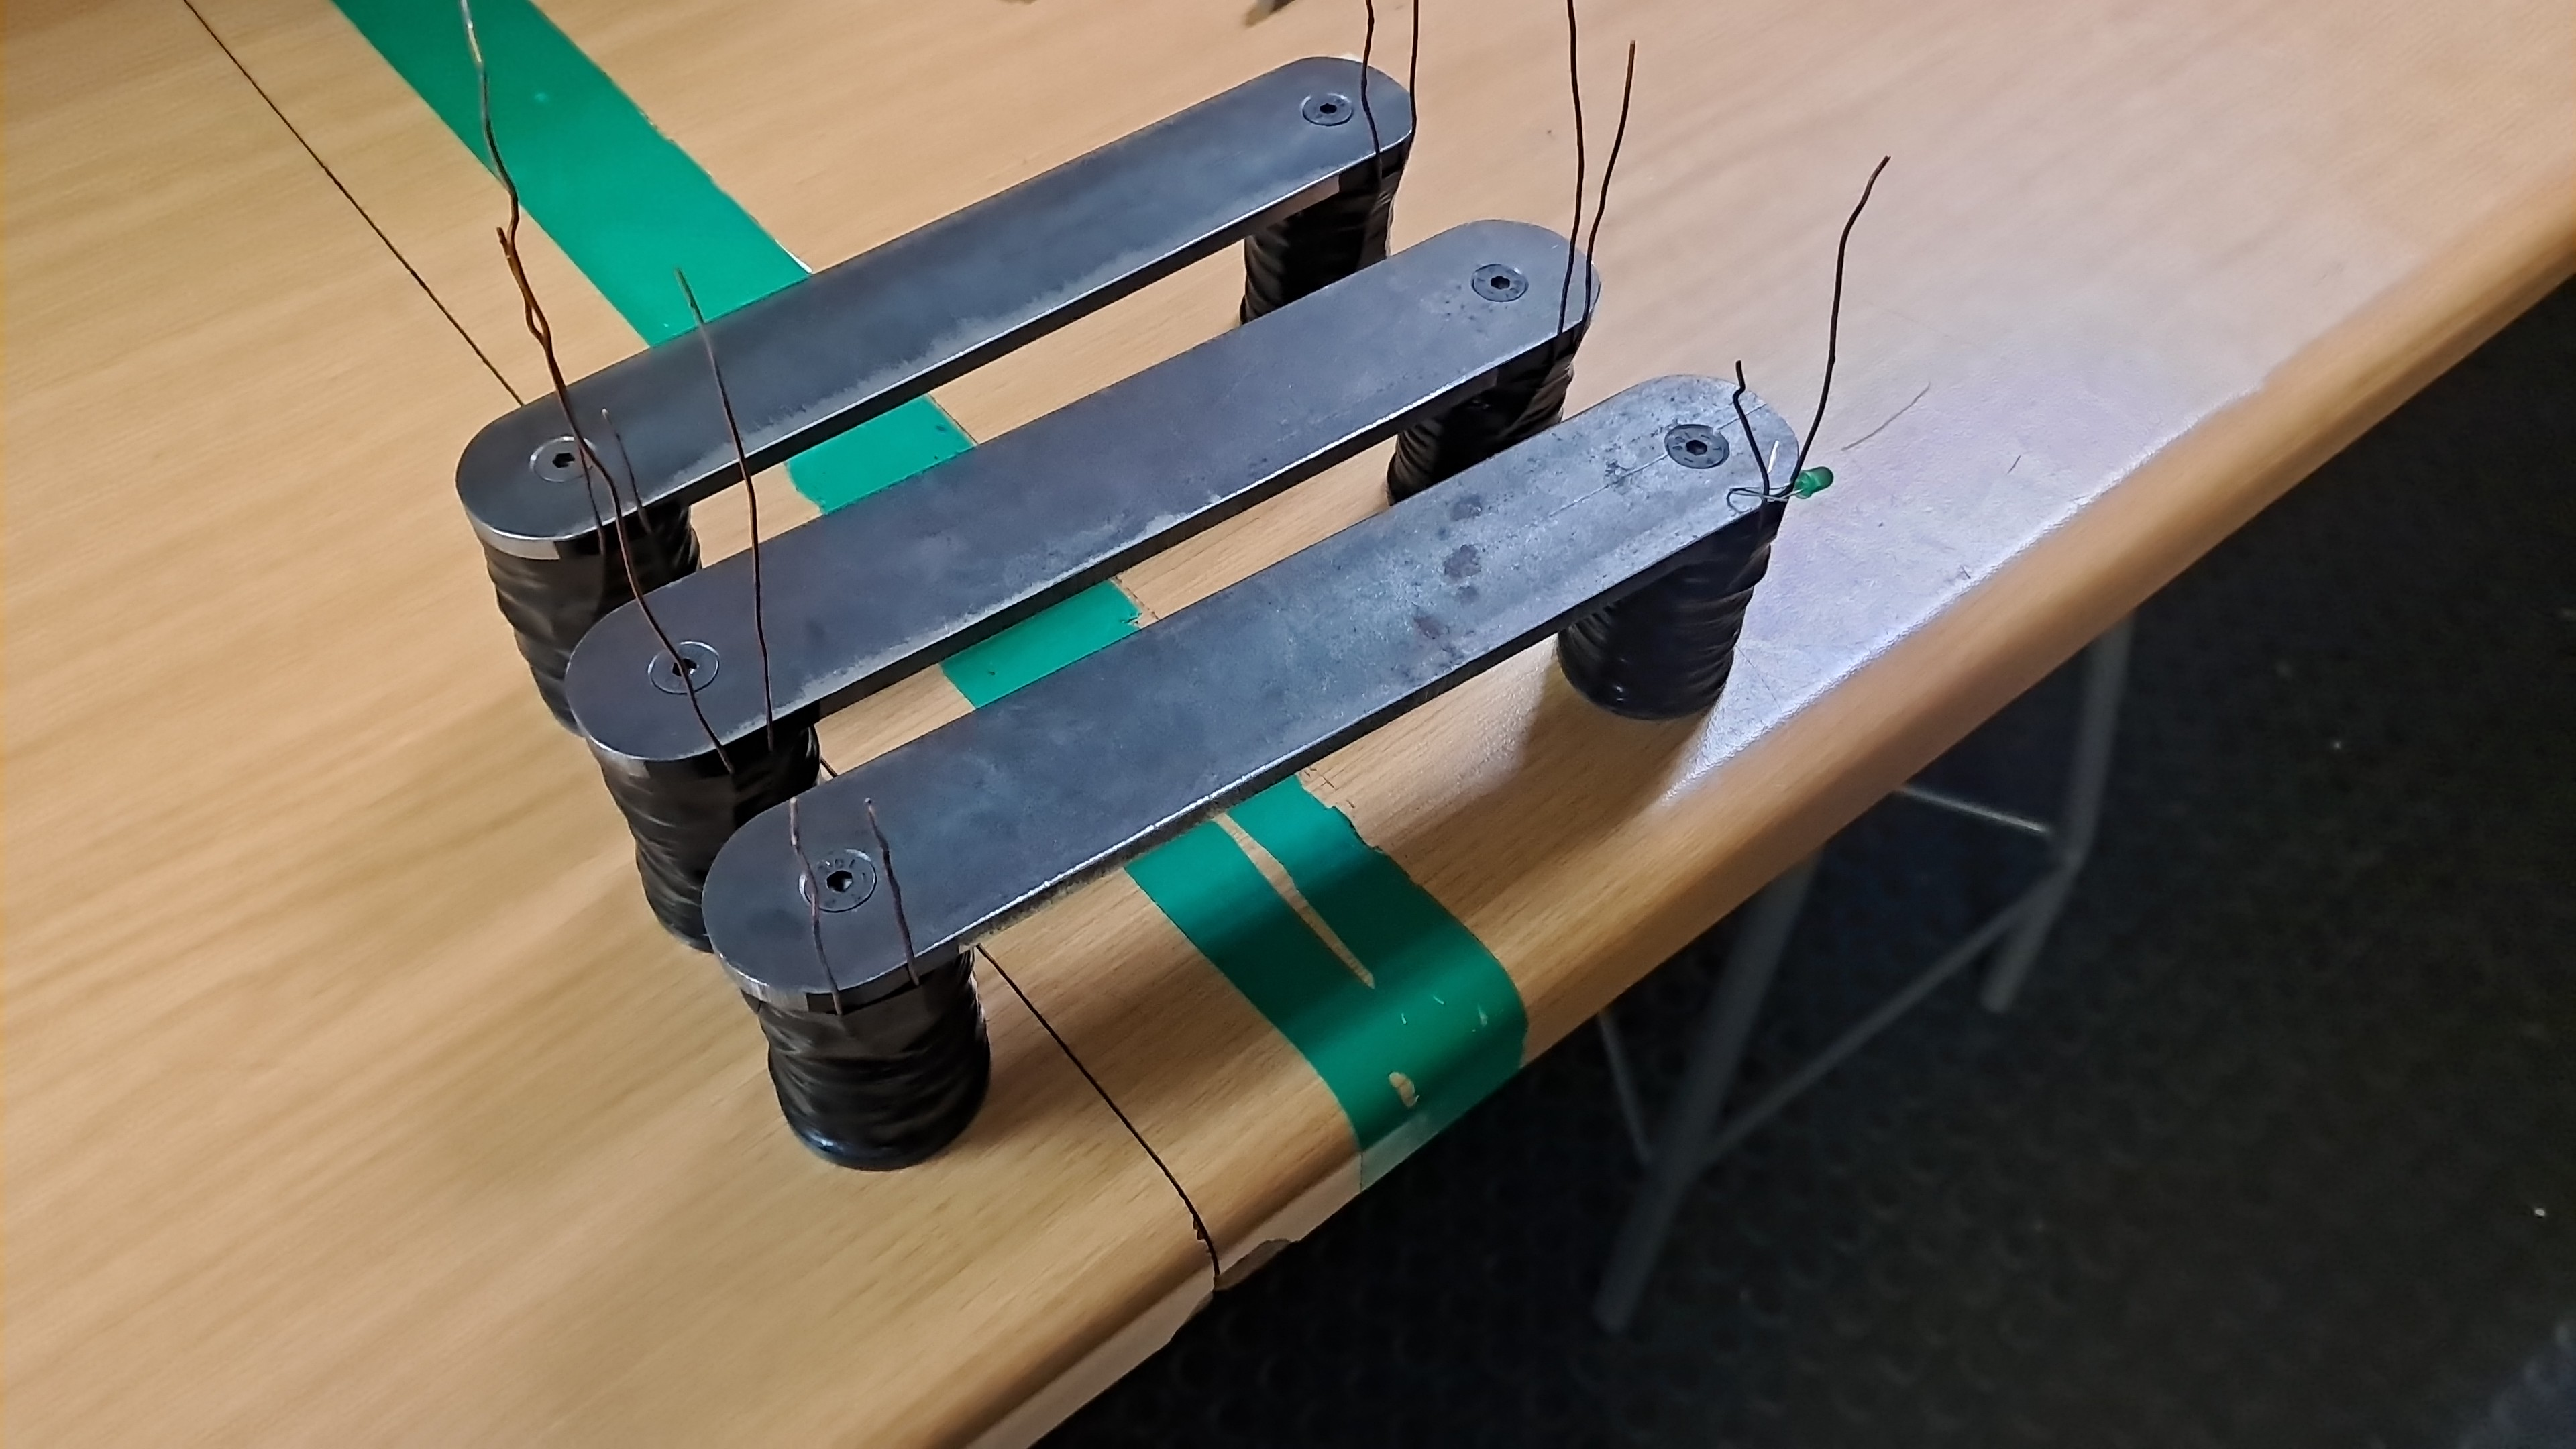
\includegraphics[width=0.95\textwidth]{figures/Magnets.jpeg}
    \caption{Physical U-core magnets}
    \label{fig:eeri2-magnet}
\end{figure}

\subsection{Power Switching and Gate Driver}
\label{subsec:eeri2-dec-driver}
The series coils have a high inductance ($L \approx 0.1\,\text{H}$ on-load) carrying $3\,\text{A}$ at $13.5\,\text{V}$.
De energising the magnet releases stored energy, causing high voltage spikes. Table~\ref{tab:eeri2-switching-tradeoff} evaluates three candidate switching technologies.

\begin{table}[H]
    \centering
    \small
    \caption{Trade-off evaluation of switching architectures.}
    \label{tab:eeri2-switching-tradeoff}
    \begin{tabularx}{\textwidth}{@{} >{\raggedright\arraybackslash}X *{5}{c} c c @{}}
        \toprule
        \textbf{Switching Architecture} & \textbf{Efficiency} & \textbf{Speed} & \textbf{Clamping} & \textbf{Life/PWM} & \textbf{Cost} & \textbf{Score} & \textbf{Selected} \\
        \textit{Criteria weighting} & \textit{0.30} & \textit{0.25} & \textit{0.20} & \textit{0.15} & \textit{0.10} & \textit{(1--5)} & \\
        \midrule
        Electromechanical relay (12\,V / 10\,A) & 4 & 1 & 2 & 1 & 5 & 2.50 & \\
        BJT (TIP120 + 1N4007)        & 2 & 2 & 2 & 3 & 4 & 2.35 & \\
        Power MOSFET (IRF540Z + TC4420 + MBR1060) & 5 & 5 & 5 & 5 & 4 & 4.90 & \checkmark \\
        \bottomrule
    \end{tabularx}
\end{table}

Electromechanical relays can arc, the contacts bounce, and it wears,
and are bad at PWM or fast emergency response.
A BJT (TIP120) exhibits a saturation voltage of 1.6, dissipating a lot of heat at $3,\text{A}$.
And the 1N4007 diode has a slow reverse recovery time ($> 2\,\mu\text{s}$) that may cause the transistor to be exposed to mutch voltage.

The combination of an IRF540Z N-channel MOSFET,
a TC4420 6\,A gate driver IC,
and an MBR1060 Schottky diode was selected.
The IRF540Z features an on-resistance of $27\,\text{m}\Omega$, this causes low conduction losses:
The TC4420 driver can source and sink up to $6\,\text{A}$ peak current directly from the $+13.5\,\text{V}$ rail, charging the gate capacitance ($C_{\mathrm{iss}} \approx 1000\,\text{pF}$) in $<25\,\text{ns}$.
This causes very low switching losses.
The MBR1060 Schottky diode ($60\,\text{V}$, $10\,\text{A}$) provides a current path across the coils.
This keeps the voltage over the switch well below the MOSFET rating ($V_{\mathrm{DSS}} = 100\,\text{V}$).

\section{MCTR I: Subsystem: Lateral Movement}
\label{sec:mctr1-subsystem-lateral-movement}

[Discuss the criteria for selecting this component (resolution,
power, size, cost, etc.). Present the options in a comparison
table.]

\begin{table}[H]
    \centering
    \caption{Available [Subsystem 1] options.}
    \label{tab:mctr1-options}
    \begin{tabular}{@{} l c c c c @{}}
        \toprule
        \textbf{Component} & \textbf{Criterion A} & \textbf{Criterion B}
            & \textbf{Criterion C} & \textbf{Selected} \\
        \midrule
        Option 1 & & & & \\
        Option 2 & & & & \checkmark \\
        Option 3 & & & & \\
        \bottomrule
    \end{tabular}
\end{table}

[Justify the selected option in one or two paragraphs.]

\begin{figure}[H]
    \centering
    %\includegraphics[width=0.40\textwidth]{subsystem1_photo}
    \caption{Selected [Subsystem 1] component.}
    \label{fig:mctr1-subsystem}
\end{figure}

\section{MCTR II: Subsystem: Spooling}
\label{sec:mctr2-subsystem-spooling}
% =====================================================================
%  mctr2_parameters.tex  --  MCTR II (Spooling) parameter + calculation sheet
%
%  HOW TO USE
%   * Edit ONLY the \In... values in Section 1. Everything in Section 2
%     (\Raw... results) is computed from them by \fpeval, so every
%     table, equation and sentence that quotes a result updates on the
%     next compile.
%   * Units are noted per line. Torques in N.m unless stated.
%   * Display helpers:  \shown{Name}{digits}        -> number only
%                       \showv{Name}{digits}{unit}  -> number + unit
%   * This file is safe to \input from several chapters (loads once).
%   * Needs: LaTeX >= 2021 (\fpeval in kernel), amsmath, xcolor.
% =====================================================================
\ifdefined\MCTRIIparamsloaded\else
\def\MCTRIIparamsloaded{}

\providecommand{\tbd}[1]{\textcolor{red}{\textbf{[TBD: #1]}}}
\newcommand{\val}[2]{\ensuremath{#1\,\mathrm{#2}}}
\newcommand{\shown}[2]{\fpeval{round(\csname Raw#1\endcsname,#2)}}
\newcommand{\showv}[3]{\val{\fpeval{round(\csname Raw#1\endcsname,#2)}}{#3}}
% PASS/FAIL helpers: \passge{value}{limit} passes when value >= limit
\newcommand{\passge}[2]{\ifdim #1pt<#2pt \textcolor{red}{\textbf{FAIL}}\else\textcolor{green!45!black}{\textbf{PASS}}\fi}
\newcommand{\passle}[2]{\ifdim #1pt>#2pt \textcolor{red}{\textbf{FAIL}}\else\textcolor{green!45!black}{\textbf{PASS}}\fi}

% Functional-unit number of MCTR II (Level 1 drawing: F/U 1.4).
% NOTE: the Level 2 drawing currently labels sub-units 1.3.x; change the
% drawing to 1.4.x (or set this to 1.3 to match the drawing, but 1.3 is MCTR I).
\newcommand{\fuMII}{1.3}

% ---------------------------------------------------------------------
% 1. INPUTS  (edit these)
% ---------------------------------------------------------------------
% -- Loads, stroke, timing
\newcommand{\InMassRated}{20}    % kg   rated payload (PHY1)
\newcommand{\InMassDesign}{30}   % kg   design overload case (analysis only)
\newcommand{\InMassAttach}{2}    % kg   magnet + hook hanging on rope  [TBD: weigh]
\newcommand{\InGrav}{9.81}       % m/s^2
\newcommand{\InStroke}{1.6}      % m     hoist stroke (PT2)
\newcommand{\InTimeReq}{20}      % s     max stroke time (PT2)
\newcommand{\InServiceF}{1.5}    % -     service factor on drum torque
\newcommand{\InSFreq}{1.5}       % -     minimum acceptable safety factor (strength checks)
% -- Drum and rope
\newcommand{\InDrumD}{50}        % mm    drum core diameter (FROZEN; 70 mm entry removed)
\newcommand{\InDrumH}{60}        % mm    drum usable length
\newcommand{\InRopeD}{5}         % mm    rope diameter
\newcommand{\InRopeCentre}{1}    % 1 = tension acts at rope centre-line (D+d); 0 = old spreadsheet (D only)
% -- Motor and VSD
\newcommand{\InMotorP}{180}      % W     Askari MS632-4
\newcommand{\InMotorN}{1360}     % rpm   at rated frequency
\newcommand{\InMotorF}{50}       % Hz    rated frequency
\newcommand{\InVsdF}{50}         % Hz    frequency VSD will actually deliver  [TBD: EEII I to confirm]
% -- Gearbox (stage A = motor side, stage B = drum side)
\newcommand{\InNpA}{16}   \newcommand{\InNgA}{102}   % pinion / gear teeth, stage A
\newcommand{\InNpB}{16}   \newcommand{\InNgB}{102}   % pinion / gear teeth, stage B
\newcommand{\InModA}{1.5} \newcommand{\InModB}{2}    % mm module
\newcommand{\InFwA}{10}   \newcommand{\InFwB}{15}    % mm face width
\newcommand{\InPhi}{25}          % deg   pressure angle (use 24 if Inventor forces it; both gears of a mesh must match)
\newcommand{\InYpA}{0.296}       % Lewis form factor, pinion  (Shigley Tbl 14-2, 20 deg value: conservative for 25 deg)
\newcommand{\InYgA}{0.447}       % Lewis form factor, gear
\newcommand{\InYpB}{0.296}
\newcommand{\InYgB}{0.447}
\newcommand{\InEta}{0.95}        % -     efficiency per gear stage
\newcommand{\InSigAllow}{20}     % MPa   allowable PETG root stress [GUESS: replace with printed-coupon result / SF]
\newcommand{\InClear}{0.25}      % mm    added centre-distance clearance (printed backlash)
\newcommand{\InBed}{220}         % mm    print bed edge length [TBD: confirm printer]
% -- Shaft, hub and fastener
\newcommand{\InShaftD}{10}       % mm    shaft diameter
\newcommand{\InSpan}{100}        % mm    bearing span (centre-to-centre)
\newcommand{\InKt}{2}            % -     bending stress-concentration factor, cross-hole
\newcommand{\InKts}{2}           % -     torsion stress-concentration factor, cross-hole
\newcommand{\InSy}{250}          % MPa   yield strength  [TBD: replace with certified grade, e.g. EN8 bright bar]
\newcommand{\InBoltD}{4}         % mm    cross-bolt diameter
\newcommand{\InHubWall}{8}       % mm    hub wall length bearing on bolt
\newcommand{\InHubAllow}{20}     % MPa   allowable PETG bearing stress [GUESS]
% -- Brake
\newcommand{\InBrakeSF}{2}       % -     brake torque safety factor
\newcommand{\InBrakeRated}{0}    % N.m   datasheet holding torque; 0 = not yet known  [TBD: datasheet]
% -- Load cell and HX711
\newcommand{\InCellCap}{100}     % kg    YZC-516 rated capacity
\newcommand{\InCellSens}{2}      % mV/V  rated output [TBD: datasheet]
\newcommand{\InExc}{5}           % V     excitation (HX711 supply)
\newcommand{\InGain}{128}        % -     HX711 channel A gain
\newcommand{\InSps}{80}          % SPS   HX711 output rate (RATE pin high)
\newcommand{\InFilt}{4}          % -     samples averaged by interlock filter
\newcommand{\InNoise}{500}       % counts peak-to-peak noise [GUESS: measure with motor running]
\newcommand{\InTrip}{1.25}       % -     overload trip as multiple of (rated + attachment)
% -- Cost (R, incl. VAT and shipping, from Cost_and_Budget.xlsx)
\newcommand{\InBudget}{5000}
\newcommand{\InCostBearings}{116.24}
\newcommand{\InCostCell}{429.00}     % [CHECK: sheet unit 493.35 + 135.70 shipping = 629.05]
\newcommand{\InCostHX}{179.40}       % [CHECK: unit price 43.70]
\newcommand{\InCostPSU}{390.17}
\newcommand{\InCostBrake}{907.68}    % excluded from the sheet's own subtotal

% ---------------------------------------------------------------------
% 2. DERIVED RESULTS  (do not edit)
% ---------------------------------------------------------------------
% -- Kinematics
\newcommand{\RawDeff}{\fpeval{\InDrumD+\InRopeCentre*\InRopeD}}
\newcommand{\RawVreq}{\fpeval{\InStroke*1000/\InTimeReq}}
\newcommand{\RawWraps}{\fpeval{\InStroke*1000/(pi*\RawDeff)}}
\newcommand{\RawWrapsFit}{\fpeval{floor(\InDrumH/\InRopeD)}}
\newcommand{\RawiA}{\fpeval{\InNgA/\InNpA}}
\newcommand{\RawiB}{\fpeval{\InNgB/\InNpB}}
\newcommand{\RawiT}{\fpeval{\RawiA*\RawiB}}
\newcommand{\RawNmot}{\fpeval{\InMotorN*\InVsdF/\InMotorF}}
\newcommand{\RawNdrum}{\fpeval{\RawNmot/\RawiT}}
\newcommand{\RawVline}{\fpeval{pi*\RawDeff*\RawNdrum/60}}
\newcommand{\RawTstroke}{\fpeval{\InStroke*1000/\RawVline}}
\newcommand{\RawSpeedMargin}{\fpeval{(\RawVline/\RawVreq-1)*100}}
\newcommand{\RawiReq}{\fpeval{pi*\RawDeff*\RawNmot/(60*\RawVreq)}}
\newcommand{\RawFmin}{\fpeval{\RawVreq*60*\RawiT/(pi*\RawDeff)*\InMotorF/\InMotorN}}
% -- Drum torque, motor sizing
\newcommand{\RawFropeR}{\fpeval{\InMassRated*\InGrav}}
\newcommand{\RawFropeD}{\fpeval{\InMassDesign*\InGrav}}
\newcommand{\RawTdrR}{\fpeval{\InMassRated*\InGrav*\RawDeff/2000}}
\newcommand{\RawTdrD}{\fpeval{\InMassDesign*\InGrav*\RawDeff/2000*\InServiceF}}
\newcommand{\RawTdrSheet}{\fpeval{\InMassDesign*\InGrav*\InDrumD/2000*\InServiceF}}
\newcommand{\RawEtaGB}{\fpeval{\InEta*\InEta}}
\newcommand{\RawTmReq}{\fpeval{\RawTdrR/(\RawiT*\RawEtaGB)}}
\newcommand{\RawTmRated}{\fpeval{\InMotorP/(2*pi*\InMotorN/60)}}
\newcommand{\RawTmMargin}{\fpeval{\RawTmRated/\RawTmReq}}
\newcommand{\RawPmech}{\fpeval{\InMassRated*\InGrav*\RawVline/1000/\RawEtaGB}}
\newcommand{\RawPavail}{\fpeval{\InMotorP*\InVsdF/\InMotorF}}
% -- Gear loads (design case) and Lewis stress
\newcommand{\RawTtwo}{\fpeval{\RawTdrD/(\RawiB*\InEta)}}
\newcommand{\RawTone}{\fpeval{\RawTtwo/(\RawiA*\InEta)}}
\newcommand{\RawFtB}{\fpeval{2*\RawTtwo*1000/(\InModB*\InNpB)}}
\newcommand{\RawFtA}{\fpeval{2*\RawTone*1000/(\InModA*\InNpA)}}
\newcommand{\RawFnB}{\fpeval{\RawFtB/cosd(\InPhi)}}
\newcommand{\RawFnA}{\fpeval{\RawFtA/cosd(\InPhi)}}
\newcommand{\RawFrB}{\fpeval{\RawFtB*tand(\InPhi)}}
\newcommand{\RawSigPA}{\fpeval{\RawFtA/(\InFwA*\InModA*\InYpA)}}
\newcommand{\RawSigGA}{\fpeval{\RawFtA/(\InFwA*\InModA*\InYgA)}}
\newcommand{\RawSigPB}{\fpeval{\RawFtB/(\InFwB*\InModB*\InYpB)}}
\newcommand{\RawSigGB}{\fpeval{\RawFtB/(\InFwB*\InModB*\InYgB)}}
\newcommand{\RawSFpA}{\fpeval{\InSigAllow/\RawSigPA}}
\newcommand{\RawSFpB}{\fpeval{\InSigAllow/\RawSigPB}}
% -- Gear geometry
\newcommand{\RawDpinA}{\fpeval{\InModA*\InNpA}}
\newcommand{\RawDgearA}{\fpeval{\InModA*\InNgA}}
\newcommand{\RawDpinB}{\fpeval{\InModB*\InNpB}}
\newcommand{\RawDgearB}{\fpeval{\InModB*\InNgB}}
\newcommand{\RawDoGearA}{\fpeval{\InModA*(\InNgA+2)}}
\newcommand{\RawDoGearB}{\fpeval{\InModB*(\InNgB+2)}}
\newcommand{\RawCdA}{\fpeval{\InModA*(\InNpA+\InNgA)/2+\InClear}}
\newcommand{\RawCdB}{\fpeval{\InModB*(\InNpB+\InNgB)/2+\InClear}}
\newcommand{\RawZmin}{\fpeval{2/(sind(\InPhi)^2)}}
\newcommand{\RawDbPinB}{\fpeval{\RawDpinB*cosd(\InPhi)}}
\newcommand{\RawBedUse}{\fpeval{max(\RawDoGearA,\RawDoGearB)/\InBed*100}}
% -- Shaft (macros with arguments: #1 = payload mass kg, #2 = torque factor)
\newcommand{\Tdr}[2]{\fpeval{#1*\InGrav*\RawDeff/2*#2}}                                   % N.mm
\newcommand{\FgB}[2]{\fpeval{2*\Tdr{#1}{#2}/(\InEta*\InModB*\InNgB*cosd(\InPhi))}}        % N
\newcommand{\Msh}[2]{\fpeval{(#1*\InGrav+\FgB{#1}{#2})*\InSpan/4}}                        % N.mm
\newcommand{\SigBsh}[2]{\fpeval{32*\Msh{#1}{#2}/(pi*\InShaftD^3)}}                        % MPa
\newcommand{\Taush}[2]{\fpeval{16*\Tdr{#1}{#2}/(pi*\InShaftD^3)}}                         % MPa
\newcommand{\VMsh}[2]{\fpeval{sqrt((\InKt*\SigBsh{#1}{#2})^2+3*(\InKts*\Taush{#1}{#2})^2)}} % MPa
\newcommand{\RawFgD}{\FgB{\InMassDesign}{\InServiceF}}
\newcommand{\RawMshD}{\Msh{\InMassDesign}{\InServiceF}}
\newcommand{\RawSigBD}{\SigBsh{\InMassDesign}{\InServiceF}}
\newcommand{\RawTauD}{\Taush{\InMassDesign}{\InServiceF}}
\newcommand{\RawVMD}{\VMsh{\InMassDesign}{\InServiceF}}
\newcommand{\RawVMR}{\VMsh{\InMassRated}{1}}
\newcommand{\RawSFsD}{\fpeval{\InSy/\RawVMD}}
\newcommand{\RawSFsR}{\fpeval{\InSy/\RawVMR}}
% -- Hub / cross-bolt (design case, drum shaft)
\newcommand{\RawFside}{\fpeval{\RawTdrD*1000/\InShaftD}}
\newcommand{\RawSigHub}{\fpeval{\RawFside/(\InBoltD*\InHubWall)}}
\newcommand{\RawTauBolt}{\fpeval{\RawFside/(pi*\InBoltD^2/4)}}
\newcommand{\RawSFhub}{\fpeval{\InHubAllow/\RawSigHub}}
% -- Rated-case (20 kg, no service factor) checks for gears and hub
\newcommand{\RawLoadRatio}{\fpeval{\RawTdrR/\RawTdrD}}
\newcommand{\RawSFpAR}{\fpeval{\RawSFpA/\RawLoadRatio}}
\newcommand{\RawSFpBR}{\fpeval{\RawSFpB/\RawLoadRatio}}
\newcommand{\RawSigHubR}{\fpeval{\RawSigHub*\RawLoadRatio}}
\newcommand{\RawSFhubR}{\fpeval{\InHubAllow/\RawSigHubR}}
% -- Brake
\newcommand{\RawTholdDrum}{\fpeval{\InMassDesign*\InGrav*\RawDeff/2000}}
\newcommand{\RawTholdIn}{\fpeval{\RawTholdDrum/\RawiT}}
\newcommand{\RawBrakeReqDrum}{\fpeval{\RawTholdDrum*\InBrakeSF}}
\newcommand{\RawBrakeReqIn}{\fpeval{\RawTholdIn*\InBrakeSF}}
\newcommand{\BrakeMarginIn}{\ifdim\InBrakeRated pt=0pt\tbd{datasheet torque}\else\fpeval{round(\InBrakeRated/\RawBrakeReqIn,1)}\fi}
\newcommand{\BrakeMarginDrum}{\ifdim\InBrakeRated pt=0pt\tbd{datasheet torque}\else\fpeval{round(\InBrakeRated/\RawBrakeReqDrum,1)}\fi}
% -- Load cell and HX711
\newcommand{\RawFcell}{\fpeval{(\InMassRated+\InMassAttach)*\InGrav}}
\newcommand{\RawMtrip}{\fpeval{(\InMassRated+\InMassAttach)*\InTrip}}
\newcommand{\RawCellUse}{\fpeval{\RawMtrip/\InCellCap*100}}
\newcommand{\RawSigFS}{\fpeval{\InCellSens*\InExc}}
\newcommand{\RawAdcRange}{\fpeval{0.5*\InExc/\InGain*1000}}
\newcommand{\RawCntPerKg}{\fpeval{\InCellSens/1000/\InCellCap*\InGain/0.5*2^23}}
\newcommand{\RawResG}{\fpeval{\InNoise/\RawCntPerKg*1000}}
\newcommand{\RawLatency}{\fpeval{\InFilt/\InSps*1000}}
\newcommand{\RawTravel}{\fpeval{\RawVline*\RawLatency/1000}}
% -- Cost
\newcommand{\RawCostTot}{\fpeval{\InCostBearings+\InCostCell+\InCostHX+\InCostPSU+\InCostBrake}}
\newcommand{\RawBudgetLeft}{\fpeval{\InBudget-\RawCostTot}}
\newcommand{\RawBudgetUse}{\fpeval{\RawCostTot/\InBudget*100}}
\fi


The spooling subsystem was selected against five criteria: \textbf{fail-safe
behaviour} (the load must be held when power or command is lost, FR6),
\textbf{compliance} with the design requirements (no worm gear, DR2; minimum
two stages), \textbf{cost} within the R\InBudget{} group cap, \textbf{manufacturability}
with the workshop tools available (3D printing, drill press), and
\textbf{verifiability} by the tests in Chapter~\ref{ch:test-plan}. All strength
figures below are produced by the parameter sheet in Appendix~\ref{app:technical};
changing an input there updates every number quoted here.
 
\subsection{Holding brake type}
\begin{table}[H]
    \centering
    \caption{Available holding-brake options for MCTR II.}
    \label{tab:mctr2-brake-type}
    \small
    \begin{tabular}{@{} l c c c c c @{}}
        \toprule
        \textbf{Option} & \textbf{Fail-safe} & \textbf{Bidirectional} & \textbf{DR2 ok}
            & \textbf{Cost} & \textbf{Selected} \\
        \midrule
        One-way (sprag) clutch            & No  & No  & Yes & Low  & \\
        Self-locking worm gear            & Yes & Yes & No  & Low  & \\
        VSD / DC-injection braking only   & No  & Yes & Yes & None & \\
        Spring-applied, electrically released brake & Yes & Yes & Yes & Medium & \checkmark \\
        \bottomrule
    \end{tabular}
\end{table}
A one-way clutch locks in one direction only, so it cannot permit powered
lowering and has no engaged or released state to monitor. A worm gear is
prohibited by DR2. Electrical braking disappears with the power it relies on.
A spring-applied brake that is released by energising its coil engages when
power is lost, which is exactly the behaviour FR6 requires.
 
\subsection{Brake source and mounting position}
A trolley drive-motor brake assembly (R\InCostBrake{} including shipping) was
chosen because the next commercially available option cost about R5\,000,
which alone would exhaust the project budget. It is released by a separate
48\,V supply.
\begin{table}[H]
    \centering
    \caption{Brake mounting position options.}
    \label{tab:mctr2-brake-pos}
    \small
    \begin{tabular}{@{} l c p{5.2cm} c @{}}
        \toprule
        \textbf{Position} & \textbf{Torque to hold} & \textbf{Protects against} & \textbf{Selected} \\
        \midrule
        Motor shaft & $<$ input value & Motor loss only; fan side not free & \\
        Gearbox input stub shaft & \showv{BrakeReqIn}{2}{N\,m} & Motor, coupling and stage~A failure & \checkmark\ (provisional) \\
        Drum shaft & \showv{BrakeReqDrum}{1}{N\,m} & Everything including gear failure & \\
        \bottomrule
    \end{tabular}
\end{table}
The input stub shaft needs only a small holding torque, which suits a
low-cost brake. The residual risk is that a stripped stage~B tooth would
release the load, and this must be accepted explicitly or the brake moved to
the drum shaft. The datasheet holding torque, coil voltage and shaft bore of the
purchased brake are not yet verified: \tbd{enter in \texttt{\textbackslash InBrakeRated}; margin is currently
\BrakeMarginIn}.
 
\subsection{Gearbox configuration and gear material}
A two-stage compound spur gearbox in 3D-printed PETG was chosen. A single
stage would violate the two-stage minimum of the work-package scope and would need
a gear of unmanageable diameter, and a planetary train is too difficult to print
with the required accuracy. Stage A (motor side) uses module \InModA\,mm and stage B
(drum side) module \InModB\,mm: stage A is limited by what a printer can form, not
by strength, while stage B carries the load. The tooth counts are
$N_p=\InNpA$, $N_g=\InNgA$ per stage, giving an overall ratio of \shown{iT}{2}:1.
Pressure angle is \InPhi$^\circ$ for every gear (both gears of a mesh must share it).
The largest gear has an outside diameter of \showv{DoGearB}{0}{mm}, which uses
\shown{BedUse}{0}\% of the assumed \InBed\,mm print bed.
 
Lewis bending stress at the rated load gives a stage~B pinion safety factor
of \shown{SFpBR}{2} against the assumed allowable of \InSigAllow\,MPa. That allowable
is a guess until a printed test pair has been loaded to failure on the test rig;
the failure torque divided by the safety factor then replaces it.
The full workings are in Appendix~\ref{app:technical}.
 
\subsection{Shaft material and gear fastening}
\begin{table}[H]
    \centering
    \caption{Options for fastening gears and drum to the shafts.}
    \label{tab:mctr2-fastening}
    \small
    \begin{tabular}{@{} l c c c c @{}}
        \toprule
        \textbf{Option} & \textbf{Makeable in workshop} & \textbf{Stiffness}
            & \textbf{Stress raiser} & \textbf{Selected} \\
        \midrule
        Taper-lock bush                         & No (needs precise taper) & High & Low    & \\
        Flexible (spider) coupling between gear and shaft & Yes & Low (backlash) & Low & \\
        Keyway in shaft                          & Hard on 10\,mm bar       & High & High   & \\
        Hub with cross-bolt through reamed hole  & Yes (drill press + jig)  & High & Medium & \checkmark \\
        \bottomrule
    \end{tabular}
\end{table}
Each gear gets a printed hub through which a bolt passes into a hole drilled
through the shaft, retained by a nut. A flexible coupling between a gear and its shaft
would add torsional compliance exactly where holding stiffness matters, so
flexible couplings are used only between the motor and the gearbox.
 
The test rig failure was traced to poor shaft design: standard steel of unknown
grade, weakened by stress concentrations from poor milling and drilling. The
following measures answer that cause directly: certified bright bar of known grade,
holes drilled and reamed on a drill press with a jig and deburred, and no holes near shoulders.
The shaft check at the design overload (\InMassDesign\,kg with service factor
\InServiceF) gives a von Mises stress of \showv{VMD}{0}{MPa} and a safety factor of
\shown{SFsD}{2}, which \ifdim\RawSFsD pt<\InSFreq pt\textcolor{red}{\textbf{does not meet}}\else meets\fi\ the
required \InSFreq. At the rated payload the safety factor is \shown{SFsR}{2}.
If the check does not close with the certified grade, the drum shaft becomes 12\,mm
(only the coupling and bearing bores change).
 
\subsection{Motor-to-gearbox coupling}
\begin{table}[H]
    \centering
    \caption{Motor coupling options.}
    \label{tab:mctr2-coupling}
    \small
    \begin{tabular}{@{} l c c c @{}}
        \toprule
        \textbf{Option} & \textbf{Absorbs misalignment} & \textbf{Protects motor bearings} & \textbf{Selected} \\
        \midrule
        Rigid coupling                      & No  & Yes if stub on bearings & \\
        Pinion overhung on motor shaft      & No  & No (gear radial load)   & \\
        Flexible jaw/spider coupling to a separately supported stub shaft & Yes & Yes & \checkmark \\
        \bottomrule
    \end{tabular}
\end{table}
The motor shaft is 11\,mm with a $4\times16$\,mm keyway and the gearbox input shaft is
\InShaftD\,mm. A coupling sized for one shaft will be bored out for the other.
Torque at this interface is only \showv{TmReq}{2}{N\,m} against a motor rating of
\showv{TmRated}{2}{N\,m}.
 
\subsection{On-hook load measurement}
\begin{table}[H]
    \centering
    \caption{Load measurement options.}
    \label{tab:mctr2-loadcell}
    \small
    \begin{tabular}{@{} l c c c @{}}
        \toprule
        \textbf{Option} & \textbf{Cost} & \textbf{Interlock speed} & \textbf{Selected} \\
        \midrule
        ADS1220 24-bit SPI ADC & Not affordable locally & High (up to 2\,kSPS) & \\
        HX711 module           & About R48              & \InSps\,SPS when RATE pin high & \checkmark \\
        \bottomrule
    \end{tabular}
\end{table}
The HX711 is selected on cost. Many modules tie the rate pin low (10\,SPS); the
purchased board must be checked and modified for \InSps\,SPS. With a
\InFilt-sample filter the detection latency is \showv{Latency}{0}{ms}, during which the
rope moves \showv{Travel}{1}{mm} at full speed. A \InCellCap\,kg S-type cell is used,
operating at \shown{CellUse}{0}\% of capacity at the overload trip. The rope passes over
a sheave suspended from the cell rather than through a fixed hook or sleeve, whose
friction would corrupt the reading. The drum-side rope leg must be horizontal so that
only the payload weight acts along the cell axis.
 
\subsection{Bearings and base plate}
Eight 6000-2RS bearings (10\,mm bore) match the shaft size. A printed housing wall is
not to rely on interference alone: a shoulder and a bolted retaining plate hold each
bearing. The baseplate is 6061-T6 aluminium with machine-cut bearing bores.
 
\subsection{Assumptions and limitations}
\begin{itemize}
    \item The payload electromagnet fails safe (or not) under the responsibility of the
          engineer for EEII~II. The hoist brake holds the rope, not the payload attachment.
    \item The assembly exists for about five days and runs for about 30 minutes, so
          creep of PETG is not considered a governing mechanism.
    \item The 30\,kg case is an analysis margin; the rated payload is \InMassRated\,kg (PHY1).
    \item The motor may not reach \InMotorN\,rpm on the custom VSD. At \InVsdF\,Hz the stroke
          takes \showv{Tstroke}{1}{s}; the VSD must deliver at least \showv{Fmin}{1}{Hz} to meet
          the \InTimeReq\,s requirement.
\end{itemize}
 
\begin{figure}[H]
    \centering
    %\includegraphics[width=0.40\textwidth]{mctr2_selected}
    \caption{Selected MCTR II components (photograph to be added).}
    \label{fig:mctr2-selected}
\end{figure}

\section{REII: Subsystem: Remote Control Dashboard}
\label{sec:reii-subsystem-remote-control-dashboard}

The proposed design prioritises reliable command delivery,
dashboard responsiveness and local fault handling.
Earlier tests used two ESP32 boards and two 1000-packet trials
per condition, at distances up to 16~m.
Table~\ref{tab:reii-options} compares the radio configurations;
Appendix~C.3 records the trial counts.
\cite{reii_measurements2026}

\begin{table}[H]
    \centering
    \footnotesize
    \caption{Available radio configurations.}
    \label{tab:reii-options}

    \begin{tabularx}{\textwidth}{@{}
        >{\raggedright\arraybackslash}p{3.5cm}
        *{4}{>{\centering\arraybackslash}X}
    @{}}
        \toprule
        \textbf{Configuration} &
        \textbf{Loss at 8~m}\newline ACK off &
        \textbf{Loss at 16~m}\newline ACK on &
        \textbf{Reported Wi-Fi channel 1 overlap} &
        \textbf{Selected} \\
        \midrule

        Channel 76, 250~kbps &
        3.30\% & 0.00\% & No & Yes \\[3pt]

        Channel 76, 2~Mbps &
        4.40\% & 0.05\% & No & No \\[3pt]

        Channel 12, 250~kbps &
        16.10\% & Not tested & Yes & No \\[3pt]

        Channel 12, 2~Mbps &
        5.50\% & Not tested & Yes & No \\

        \bottomrule
    \end{tabularx}
\end{table}

\noindent
\textbf{Radio configuration.}
Channel 76 and 250~kbps are provisionally selected for lower
packet loss at longer tested distances, favouring reliable
delivery over nominal data rate. Channel 12 overlapped the
reported laboratory Wi-Fi allocation. Acknowledgements and
retries improved delivery in the earlier tests.
\cite{reii_measurements2026}
The runtime power setting of 2 and final ESP32-S3 response
times still require validation.

\noindent
\textbf{Communication and local control.}
Communication is handled separately from the dashboard
controls to keep the interface responsive while waiting
for replies. Messages have a fixed length of 32 bytes to
simplify processing. A radio acknowledgement confirms
message delivery; a separate controller reply indicates
whether the command was accepted. The ESP32-S3 would
generate control outputs and respond to communication
loss locally. The dashboard would calculate anti-sway
motion profiles and paths around known obstacles, which
the controller would execute through MCTR I's lateral
drive.
\cite{nwu_reii_scope2026}
These functions still require validation.

\noindent
\textbf{Starting reference.}
Marked upper-hoist parking with clearance and a marked
trolley position would provide a repeatable starting
condition. While stationary and disarmed, the operator
would select \emph{Confirm starting position} to set
the lateral reference before arming, without automatic
movement. Encoder feedback would then track lateral
position. This feature remains to be implemented.

\begin{figure}[H]
    \centering
    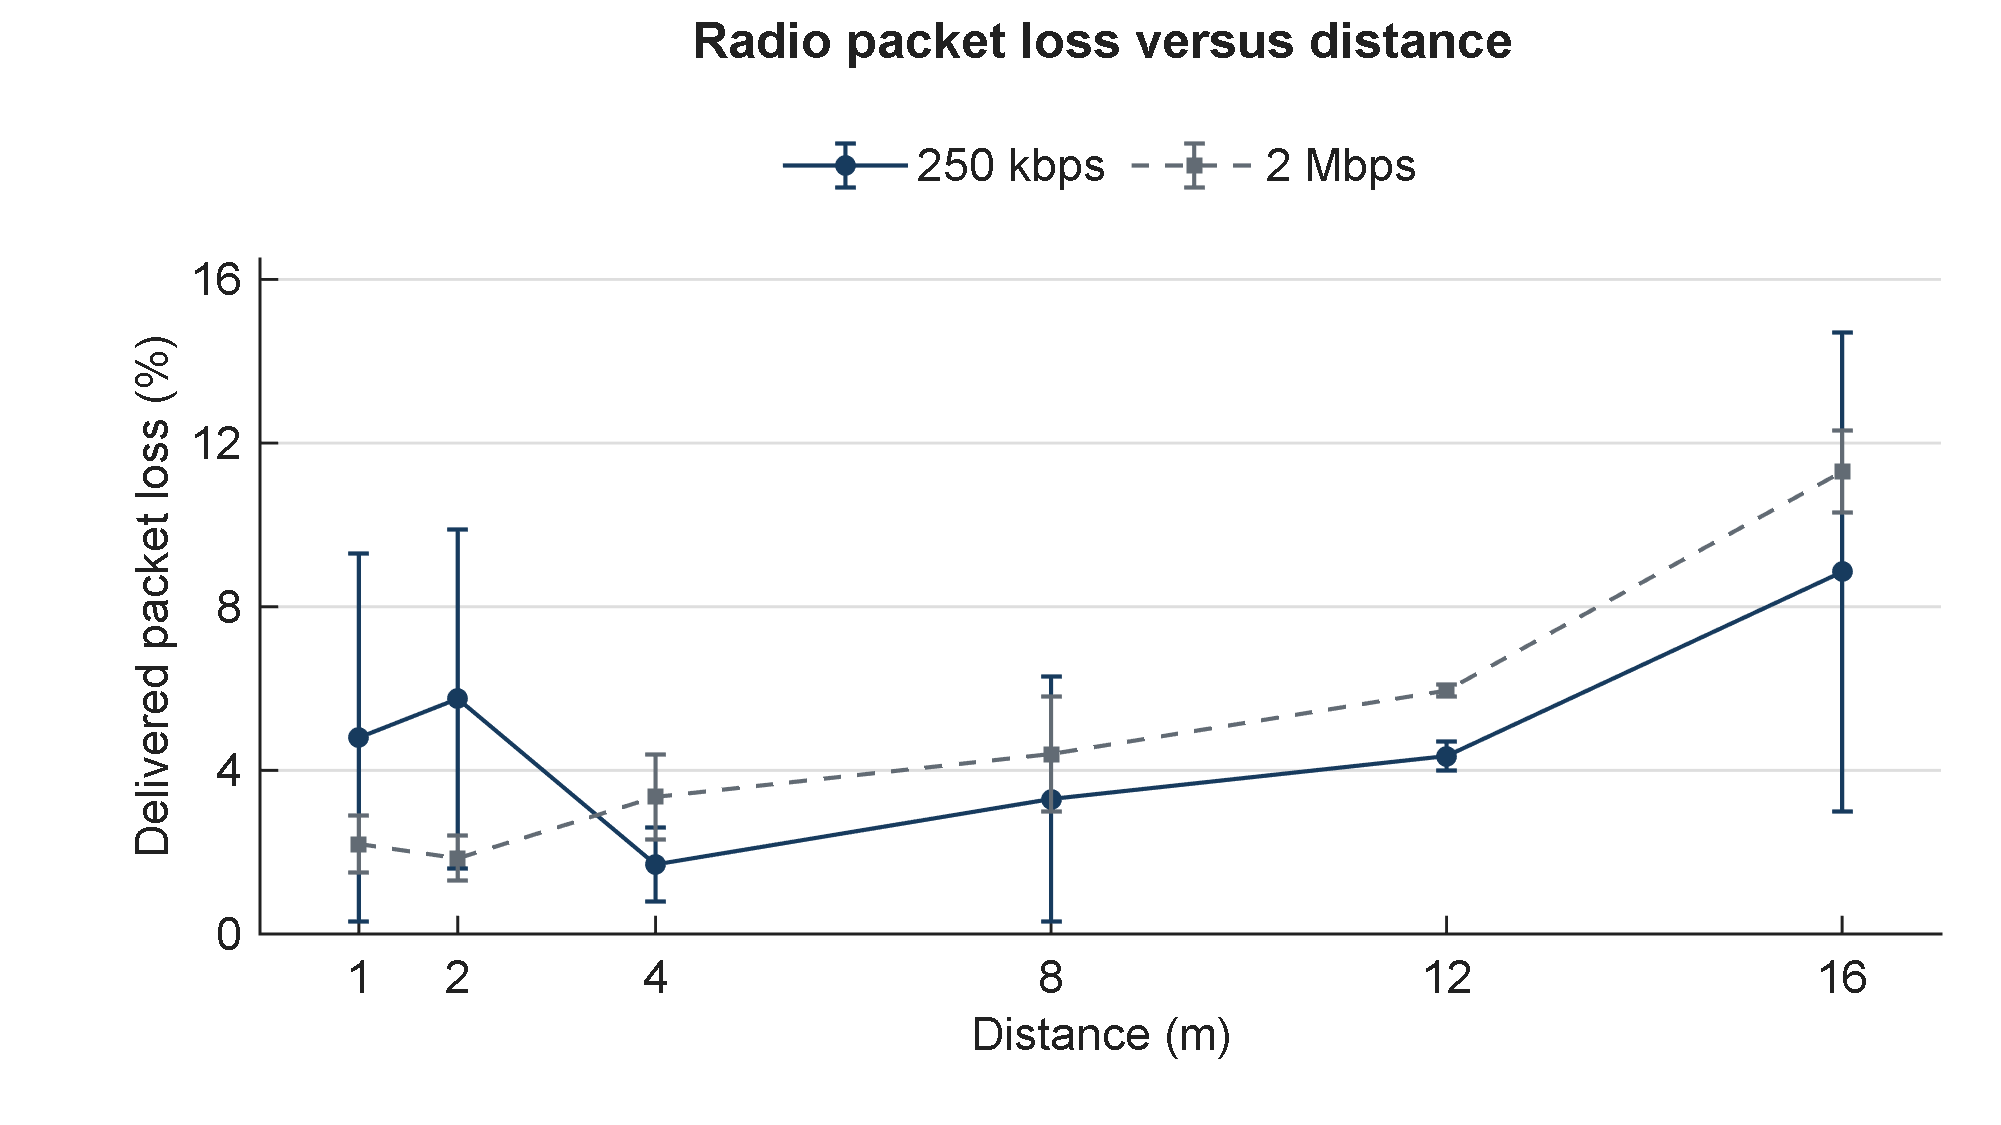
\includegraphics[width=0.80\textwidth]
        {figures/Figure_5_5_Radio_Performance.png}
    \caption{Radio packet loss versus distance on channel 76,
        supporting the provisional 250~kbps selection.
        Acknowledgements and retries were disabled.
        Points are means of two trials; bars show the
        two trial values.
        \cite{reii_measurements2026}}
    \label{fig:reii-subsystem}
\end{figure}
% ============================================================
%  CHAPTER 6 – TEST PLAN
% ============================================================
\chapter{Test Plan}
\label{ch:test-plan}
This chapter discusses the individual subsystem verification test plans (Section~\ref{sec:individual-tests}), subsystem integration testing (Section~\ref{sec:integration-tests}), and full-system validation (Section~\ref{sec:system-validation}) to be implemented to ensure the functioning of each subsystem as a whole. The persons responsible for collaboration on the test plan are the 2 persons who have the role in the subsection title. Testing is divided into individual subsystem verification,
subsystem integration testing, and full-system validation.

Each test shall specify the initial conditions, test procedure,
expected result, and acceptance criteria. The actual result and
test status shall be recorded during execution.

\section{Test Procedure and Acceptance Criteria}
The following information shall be documented for each test:
\begin{itemize}
    \item \textbf{Test ID:} A unique identifier for the test.
    \item \textbf{Objective:} The functionality or requirement
    being verified.
    \item \textbf{Initial conditions:} The required system
    configuration before testing.
    \item \textbf{Procedure:} The steps followed to perform the test.
    \item \textbf{Expected result:} The anticipated system response.
    \item \textbf{Acceptance criteria:} The measurable conditions
    required for the test to pass.
    \item \textbf{Actual result:} The observed outcome.
    \item \textbf{Status:} Pass, Fail, or Not Tested.
\end{itemize}

\section{Individual Test Plans}
\label{sec:individual-tests}

Each subsystem shall first be tested independently, where
practical, to establish that its functionality meets the
specified design requirements before integration testing.


\subsection{EERI I}
\label{subsec:eeri-i-tests}

\textbf{Subsystem function:} [Insert the function of EERI I.]

\textbf{Test setup:} [Insert the required equipment, configuration,
and initial conditions.]

\begin{table}[htbp]
    \centering
    \caption{EERI I test plan}
    \label{tab:eeri-i-tests}
    \renewcommand{\arraystretch}{1.4}
    \begin{tabularx}{\textwidth}{|l|X|X|X|X|}
        \hline
        \textbf{Test ID} &
        \textbf{Test description} &
        \textbf{Procedure} &
        \textbf{Expected result} &
        \textbf{Status} \\
        \hline
        EI-01 & [Functional test] &
        [Test procedure] &
        [Expected behaviour] &
        [Pass/Fail/NT] \\
        \hline
        EI-02 & [Performance test] &
        [Test procedure] &
        [Acceptance criterion] &
        [Pass/Fail/NT] \\
        \hline
        EI-03 & [Safety or fault test] &
        [Test procedure] &
        [Expected safe response] &
        [Pass/Fail/NT] \\
        \hline
    \end{tabularx}
\end{table}


\subsection{EERI II}
\label{subsec:eeri-ii-tests}

\textbf{Subsystem function:} [Insert the function of EERI II.]

\textbf{Test setup:} [Insert the required equipment, configuration,
and initial conditions.]

\begin{table}[htbp]
    \centering
    \caption{EERI II test plan}
    \label{tab:eeri-ii-tests}
    \renewcommand{\arraystretch}{1.4}
    \begin{tabularx}{\textwidth}{|l|X|X|X|X|}
        \hline
        \textbf{Test ID} &
        \textbf{Test description} &
        \textbf{Procedure} &
        \textbf{Expected result} &
        \textbf{Status} \\
        \hline
        EII-01 & [Functional test] &
        [Test procedure] &
        [Expected behaviour] &
        [Pass/Fail/NT] \\
        \hline
        EII-02 & [Performance test] &
        [Test procedure] &
        [Acceptance criterion] &
        [Pass/Fail/NT] \\
        \hline
        EII-03 & [Safety or fault test] &
        [Test procedure] &
        [Expected safe response] &
        [Pass/Fail/NT] \\
        \hline
    \end{tabularx}
\end{table}


\subsection{MCTR I}
\label{subsec:mctr-i-tests}

\textbf{Subsystem function:} [Insert the function of MCTR I.]

\textbf{Test setup:} [Insert the required equipment, configuration,
and initial conditions.]

\begin{table}[htbp]
    \centering
    \caption{MCTR I test plan}
    \label{tab:mctr-i-tests}
    \renewcommand{\arraystretch}{1.4}
    \begin{tabularx}{\textwidth}{|l|X|X|X|X|}
        \hline
        \textbf{Test ID} &
        \textbf{Test description} &
        \textbf{Procedure} &
        \textbf{Expected result} &
        \textbf{Status} \\
        \hline
        MCI-01 & [Functional test] &
        [Test procedure] &
        [Expected behaviour] &
        [Pass/Fail/NT] \\
        \hline
        MCI-02 & [Performance test] &
        [Test procedure] &
        [Acceptance criterion] &
        [Pass/Fail/NT] \\
        \hline
        MCI-03 & [Safety or fault test] &
        [Test procedure] &
        [Expected safe response] &
        [Pass/Fail/NT] \\
        \hline
    \end{tabularx}
\end{table}


\subsection{MCTR II}
\label{subsec:mctr-ii-tests}

\textbf{Subsystem function:} [Insert the function of MCTR II.]

\textbf{Test setup:} [Insert the required equipment, configuration,
and initial conditions.]

\begin{table}[htbp]
    \centering
    \caption{MCTR II test plan}
    \label{tab:mctr-ii-tests}
    \renewcommand{\arraystretch}{1.4}
    \begin{tabularx}{\textwidth}{|l|X|X|X|X|}
        \hline
        \textbf{Test ID} &
        \textbf{Test description} &
        \textbf{Procedure} &
        \textbf{Expected result} &
        \textbf{Status} \\
        \hline
        MCII-01 & [Functional test] &
        [Test procedure] &
        [Expected behaviour] &
        [Pass/Fail/NT] \\
        \hline
        MCII-02 & [Performance test] &
        [Test procedure] &
        [Acceptance criterion] &
        [Pass/Fail/NT] \\
        \hline
        MCII-03 & [Safety or fault test] &
        [Test procedure] &
        [Expected safe response] &
        [Pass/Fail/NT] \\
        \hline
    \end{tabularx}
\end{table}


\subsection{REII}
\label{subsec:reii-tests}

\textbf{Subsystem function:} [Insert the function of REII.]

\textbf{Test setup:} [Insert the required equipment, configuration,
and initial conditions.]

\begin{table}[htbp]
    \centering
    \caption{REII test plan}
    \label{tab:reii-tests}
    \renewcommand{\arraystretch}{1.4}
    \begin{tabularx}{\textwidth}{|l|X|X|X|X|}
        \hline
        \textbf{Test ID} &
        \textbf{Test description} &
        \textbf{Procedure} &
        \textbf{Expected result} &
        \textbf{Status} \\
        \hline
        RE-01 & [Functional test] &
        [Test procedure] &
        [Expected behaviour] &
        [Pass/Fail/NT] \\
        \hline
        RE-02 & [Performance test] &
        [Test procedure] &
        [Acceptance criterion] &
        [Pass/Fail/NT] \\
        \hline
        RE-03 & [Safety or fault test] &
        [Test procedure] &
        [Expected safe response] &
        [Pass/Fail/NT] \\
        \hline
    \end{tabularx}
\end{table}

\section{Subsystem Interface Analysis}
\label{sec:interface-analysis}

The subsystem interface analysis identifies the direct interactions
between subsystems. These interfaces may involve mechanical loads,
electrical power, control signals, communication, or physical
connections, as applicable to the design.

\begin{table}[htbp]
    \centering
    \caption{Subsystem interface matrix}
    \label{tab:interface-matrix}
    \renewcommand{\arraystretch}{1.4}
    \begin{tabularx}{\textwidth}{|X|c|c|c|c|c|}
        \hline
        \textbf{Subsystem} &
        \textbf{EERI I} &
        \textbf{EERI II} &
        \textbf{MCTR I} &
        \textbf{MCTR II} &
        \textbf{REII} \\
        \hline
        EERI I   & -- & [X] & [X] & [X] & [X] \\
        \hline
        EERI II  & [X] & -- & [X] & [X] & [X] \\
        \hline
        MCTR I   & [X] & [X] & -- & [X] & [X] \\
        \hline
        MCTR II  & [X] & [X] & [X] & -- & [X] \\
        \hline
        REII     & [X] & [X] & [X] & [X] & -- \\
        \hline
    \end{tabularx}
\end{table}

In Table~\ref{tab:interface-matrix}, replace \texttt{[X]} with
\texttt{X} where a direct interface exists and leave the cell
blank where no direct interface exists. The matrix shall be
used to determine the required integration tests.

\section{Subsystem Integration Test Plan}
\label{sec:integration-tests}

Integration testing verifies that connected subsystems operate
together correctly and that their interfaces satisfy the design
requirements. Testing shall be performed after the relevant
individual subsystem tests have been completed.

\begin{table}[htbp]
    \centering
    \caption{Subsystem integration test plan}
    \label{tab:integration-tests}
    \renewcommand{\arraystretch}{1.4}
    \begin{tabularx}{\textwidth}{|l|X|X|X|X|}
        \hline
        \textbf{Test ID} &
        \textbf{Subsystems} &
        \textbf{Test objective} &
        \textbf{Expected result} &
        \textbf{Status} \\
        \hline
        INT-01 & [Subsystem A and B] &
        Verify the interface between the subsystems &
        [Specified interface behaviour] &
        [Pass/Fail/NT] \\
        \hline
        INT-02 & [Subsystem A and C] &
        Verify coordinated operation &
        [Specified response] &
        [Pass/Fail/NT] \\
        \hline
        INT-03 & [Subsystem B and D] &
        Verify signal, load, or power transfer, as applicable &
        [Specified transfer behaviour] &
        [Pass/Fail/NT] \\
        \hline
        INT-04 & [Relevant subsystems] &
        Verify a multi-subsystem operating sequence &
        [Specified sequence completed correctly] &
        [Pass/Fail/NT] \\
        \hline
        INT-05 & [Relevant subsystems] &
        Verify fault propagation and safe response &
        [Specified fault-handling behaviour] &
        [Pass/Fail/NT] \\
        \hline
    \end{tabularx}
\end{table}

For each integration test, record the initial conditions, test
procedure, measured or observed results, and applicable
acceptance criteria. Tests shall cover every required interface
identified in Table~\ref{tab:interface-matrix}.


\section{Full-System Validation}
\label{sec:system-validation}

Full-system validation shall be conducted after the individual
subsystem and integration tests have been completed. The purpose
is to determine whether the complete gantry crane system satisfies
its overall functional, performance, and safety requirements.

\begin{table}[htbp]
    \centering
    \caption{Full-system validation plan}
    \label{tab:system-validation}
    \renewcommand{\arraystretch}{1.4}
    \begin{tabularx}{\textwidth}{|l|X|X|X|}
        \hline
        \textbf{Test ID} &
        \textbf{Test scenario} &
        \textbf{Acceptance criteria} &
        \textbf{Status} \\
        \hline
        SYS-01 & Normal startup and shutdown &
        [System starts and stops as specified] &
        [Pass/Fail/NT] \\
        \hline
        SYS-02 & Complete operating cycle &
        [Required sequence is completed] &
        [Pass/Fail/NT] \\
        \hline
        SYS-03 & Operation under specified load &
        [Performance remains within limits] &
        [Pass/Fail/NT] \\
        \hline
        SYS-04 & Fault handling and emergency stop &
        [Required safe response is achieved] &
        [Pass/Fail/NT] \\
        \hline
        SYS-05 & Repeated operation &
        [Required repeatability or reliability criteria] &
        [Pass/Fail/NT] \\
        \hline
    \end{tabularx}
\end{table}


\section{Test Results Summary}
\label{sec:test-results-summary}

The results of the subsystem, integration, and full-system tests
shall be consolidated to assess overall system readiness.

\begin{table}[htbp]
    \centering
    \caption{Summary of test outcomes}
    \label{tab:test-summary}
    \renewcommand{\arraystretch}{1.4}
    \begin{tabularx}{\textwidth}{|X|c|c|c|c|}
        \hline
        \textbf{Test category} &
        \textbf{Passed} &
        \textbf{Failed} &
        \textbf{Not tested} &
        \textbf{Total} \\
        \hline
        Individual subsystem tests & [\,] & [\,] & [\,] & [\,] \\
        \hline
        Integration tests & [\,] & [\,] & [\,] & [\,] \\
        \hline
        Full-system validation & [\,] & [\,] & [\,] & [\,] \\
        \hline
        \textbf{Total} & [\,] & [\,] & [\,] & [\,] \\
        \hline
    \end{tabularx}
\end{table}

Any failed or incomplete tests shall be documented together with
the observed behaviour, likely cause, corrective action, and
retesting requirements. The system shall only be declared to have
passed validation when the applicable acceptance criteria have
been met.


% ============================================================
%  CHAPTER 7 -- System Performance
% ============================================================
\chapter{System Performance}
\label{ch:system-performance}

This chapter evaluates the performance of the five subsystems
comprising the gantry crane system: EERI I, EERI II, MCTR I,
MCTR II, and REII. The performance of each subsystem is assessed
against its design requirements using appropriate measurable
indicators and verification methods. The interactions between
subsystems are also considered to determine whether the integrated
system satisfies the overall design objectives.

\section{Performance Evaluation Methodology}
\label{sec:performance-methodology}

The performance of each subsystem shall be evaluated by comparing
its specified design requirements with the results obtained during
testing. Each performance indicator shall have a defined target,
a measurement method, and an acceptance criterion.

The following information shall be recorded for each indicator:
\begin{itemize}
    \item \textbf{Design requirement:} The required subsystem
    functionality or performance.
    \item \textbf{Performance indicator:} The measurable quantity
    used to evaluate the requirement.
    \item \textbf{Target value:} The value or operating range
    specified during the design process.
    \item \textbf{Measured result:} The value obtained during testing.
    \item \textbf{Assessment:} Whether the measured result satisfies
    the specified acceptance criterion.
\end{itemize}

\section{EERI I Performance}
\label{sec:eeri-i-performance}

This section evaluates the performance of EERI I with respect to
its assigned function within the gantry crane system. The indicators
selected for evaluation shall correspond to the subsystem's
functional and engineering requirements.

\begin{table}[H]
    \centering
    \caption{Performance indicators for EERI I.}
    \label{tab:eeri-i-performance}
    \renewcommand{\arraystretch}{1.4}
    \begin{tabularx}{\textwidth}{|X|X|X|X|}
        \hline
        \textbf{Performance indicator} &
        \textbf{Target value} &
        \textbf{Measured result} &
        \textbf{Assessment} \\
        \hline
        Primary functional performance &
        [Specified target] &
        [Measured result] &
        [Pass/Fail] \\
        \hline
        Operational accuracy or output quality &
        [Specified target] &
        [Measured result] &
        [Pass/Fail] \\
        \hline
        Response time or operating speed &
        [Specified target] &
        [Measured result] &
        [Pass/Fail] \\
        \hline
        Power consumption or operating efficiency,
        where applicable &
        [Specified target] &
        [Measured result] &
        [Pass/Fail] \\
        \hline
        Reliability under specified operating conditions &
        [Specified target] &
        [Measured result] &
        [Pass/Fail] \\
        \hline
    \end{tabularx}
\end{table}

The results shall be used to determine whether EERI I satisfies
its allocated requirements. Any deviations from the target values
shall be documented together with their probable causes and
effects on the overall system.

\section{EERI II Performance}
\label{sec:eeri-ii-performance}

The performance of EERI II shall be assessed according to its
role in the gantry crane system. Particular attention shall be
given to its principal function, the consistency of its output,
and its ability to operate within the specified design limits.

\begin{table}[H]
    \centering
    \caption{Performance indicators for EERI II.}
    \label{tab:eeri-ii-performance}
    \renewcommand{\arraystretch}{1.4}
    \begin{tabularx}{\textwidth}{|X|X|X|X|}
        \hline
        \textbf{Performance indicator} &
        \textbf{Target value} &
        \textbf{Measured result} &
        \textbf{Assessment} \\
        \hline
        Primary functional performance &
        [Specified target] &
        [Measured result] &
        [Pass/Fail] \\
        \hline
        Output accuracy or consistency &
        [Specified target] &
        [Measured result] &
        [Pass/Fail] \\
        \hline
        Response time or operating speed &
        [Specified target] &
        [Measured result] &
        [Pass/Fail] \\
        \hline
        Operating range or capacity, where applicable &
        [Specified target] &
        [Measured result] &
        [Pass/Fail] \\
        \hline
        Reliability under specified operating conditions &
        [Specified target] &
        [Measured result] &
        [Pass/Fail] \\
        \hline
    \end{tabularx}
\end{table}

The measured results shall establish whether EERI II performs
within its required operating range and whether its output is
suitable for the subsystem or subsystems with which it interacts.

\section{MCTR I Performance}
\label{sec:mctr-i-performance}

This section evaluates MCTR I in terms of its principal function
and its contribution to the mechanical and operational performance
of the gantry crane. Where applicable, the assessment shall include
load capacity, positional accuracy, motion, structural behaviour,
or other indicators relevant to the subsystem's actual design.

\begin{table}[H]
    \centering
    \caption{Performance indicators for MCTR I.}
    \label{tab:mctr-i-performance}
    \renewcommand{\arraystretch}{1.4}
    \begin{tabularx}{\textwidth}{|X|X|X|X|}
        \hline
        \textbf{Performance indicator} &
        \textbf{Target value} &
        \textbf{Measured result} &
        \textbf{Assessment} \\
        \hline
        Primary functional performance &
        [Specified target] &
        [Measured result] &
        [Pass/Fail] \\
        \hline
        Load capacity or operating capacity,
        where applicable &
        [Specified target] &
        [Measured result] &
        [Pass/Fail] \\
        \hline
        Positional accuracy or dimensional tolerance,
        where applicable &
        [Specified target] &
        [Measured result] &
        [Pass/Fail] \\
        \hline
        Operating speed or cycle time,
        where applicable &
        [Specified target] &
        [Measured result] &
        [Pass/Fail] \\
        \hline
        Mechanical integrity or stability,
        where applicable &
        [Specified criterion] &
        [Observed result] &
        [Pass/Fail] \\
        \hline
    \end{tabularx}
\end{table}

The results shall indicate whether MCTR I meets its required
functional and mechanical performance. Any observed deflection,
misalignment, excessive friction, instability, or other deviation
shall be documented where relevant to the subsystem.

\section{MCTR II Performance}
\label{sec:mctr-ii-performance}

MCTR II shall be evaluated against the requirements associated
with its assigned function. The assessment shall consider its
operational performance and any relevant mechanical, electrical,
or control-related characteristics.

\begin{table}[H]
    \centering
    \caption{Performance indicators for MCTR II.}
    \label{tab:mctr-ii-performance}
    \renewcommand{\arraystretch}{1.4}
    \begin{tabularx}{\textwidth}{|X|X|X|X|}
        \hline
        \textbf{Performance indicator} &
        \textbf{Target value} &
        \textbf{Measured result} &
        \textbf{Assessment} \\
        \hline
        Primary functional performance &
        [Specified target] &
        [Measured result] &
        [Pass/Fail] \\
        \hline
        Operating capacity or load handling,
        where applicable &
        [Specified target] &
        [Measured result] &
        [Pass/Fail] \\
        \hline
        Positioning accuracy or repeatability,
        where applicable &
        [Specified target] &
        [Measured result] &
        [Pass/Fail] \\
        \hline
        Response time or operating cycle time &
        [Specified target] &
        [Measured result] &
        [Pass/Fail] \\
        \hline
        Reliability and safe operation under
        specified conditions &
        [Specified criterion] &
        [Observed result] &
        [Pass/Fail] \\
        \hline
    \end{tabularx}
\end{table}

The results shall be compared with those of MCTR I where the
subsystems have related functions or operate together. This
comparison shall identify any performance differences that affect
the coordinated operation of the gantry crane.

\section{REII Performance}
\label{sec:reii-performance}

Final performance testing of the ESP32-S3-based REII
subsystem has not yet been completed. Earlier ESP32
radio measurements provide preliminary communication
results but do not establish integrated crane performance.
\cite{reii_measurements2026}

\begin{table}[H]
    \centering
    \caption{Performance indicators for REII.}
    \label{tab:reii-performance}
    \renewcommand{\arraystretch}{1.4}
    \begin{tabularx}{\textwidth}{|X|X|X|X|}
        \hline
        \textbf{Performance indicator} &
        \textbf{Target value} &
        \textbf{Measured result} &
        \textbf{Assessment} \\
        \hline
        Primary functional performance &
        [Specified target] &
        [Measured result] &
        [Pass/Fail] \\
        \hline
        Output accuracy or operational effectiveness &
        [Specified target] &
        [Measured result] &
        [Pass/Fail] \\
        \hline
        Response time or operating speed,
        where applicable &
        [Specified target] &
        [Measured result] &
        [Pass/Fail] \\
        \hline
        Operating capacity or efficiency,
        where applicable &
        [Specified target] &
        [Measured result] &
        [Pass/Fail] \\
        \hline
        Reliability or required safe response &
        [Specified criterion] &
        [Observed result] &
        [Pass/Fail] \\
        \hline
    \end{tabularx}
\end{table}

The results shall establish whether REII satisfies its allocated
requirements and whether its operation introduces any limitations
or dependencies affecting the performance of the complete system.

\section{Integrated System Performance}
\label{sec:integrated-performance}

The integrated performance assessment considers the interactions
between EERI I, EERI II, MCTR I, MCTR II, and REII. Individual
subsystem performance does not necessarily guarantee correct
system operation; therefore, the interfaces and coordinated
operating sequences shall also be evaluated.

\begin{table}[H]
    \centering
    \caption{Integrated system performance indicators.}
    \label{tab:integrated-performance}
    \renewcommand{\arraystretch}{1.4}
    \begin{tabularx}{\textwidth}{|X|X|X|X|}
        \hline
        \textbf{Performance indicator} &
        \textbf{Target value} &
        \textbf{Measured result} &
        \textbf{Assessment} \\
        \hline
        Correct operation of subsystem interfaces &
        [Specified criterion] &
        [Observed result] &
        [Pass/Fail] \\
        \hline
        Completion of the required operating sequence &
        [Specified criterion] &
        [Observed result] &
        [Pass/Fail] \\
        \hline
        Overall operating time or cycle time &
        [Specified target] &
        [Measured result] &
        [Pass/Fail] \\
        \hline
        System performance under the specified load
        or operating conditions &
        [Specified target] &
        [Measured result] &
        [Pass/Fail] \\
        \hline
        Fault handling and required safe-state behaviour &
        [Specified criterion] &
        [Observed result] &
        [Pass/Fail] \\
        \hline
    \end{tabularx}
\end{table}

Integration testing shall verify that signals, loads, power, and
other relevant quantities are transferred correctly across each
required interface. The complete operating sequence shall be
evaluated to identify delays, incompatibilities, or performance
limitations arising from interactions between subsystems.

\section{Summary of System Performance}
\label{sec:system-performance-summary}

The performance results for all five subsystems and the integrated
system shall be consolidated to assess compliance with the design
requirements.

\begin{table}[H]
    \centering
    \caption{Summary of subsystem performance.}
    \label{tab:system-performance-summary}
    \renewcommand{\arraystretch}{1.4}
    \begin{tabularx}{\textwidth}{|X|X|X|X|}
        \hline
        \textbf{Subsystem} &
        \textbf{Requirements assessed} &
        \textbf{Requirements satisfied} &
        \textbf{Outstanding issues} \\
        \hline
        EERI I & [Number or reference] &
        [Number or percentage] & [Details] \\
        \hline
        EERI II & [Number or reference] &
        [Number or percentage] & [Details] \\
        \hline
        MCTR I & [Number or reference] &
        [Number or percentage] & [Details] \\
        \hline
        MCTR II & [Number or reference] &
        [Number or percentage] & [Details] \\
        \hline
        REII & [Number or reference] &
        [Number or percentage] & [Details] \\
        \hline
        Integrated system & [Number or reference] &
        [Number or percentage] & [Details] \\
        \hline
    \end{tabularx}
\end{table}

The final assessment shall identify which requirements have been
satisfied, which remain outstanding, and whether corrective action
or further testing is required. The system shall be considered to
meet its performance objectives only when the relevant acceptance
criteria have been demonstrated by the recorded results.


% ============================================================
%  CHAPTER 8 -- Implementation Evidence
% ============================================================
\chapter{Implementation Evidence}
\label{ch:implementation-evidence}

This chapter presents the evidence of the physical and functional
implementation of the gantry crane system. Evidence is provided
for each of the five subsystems, namely EERI I, EERI II, MCTR I,
MCTR II, and REII, followed by evidence of the integrated system.
The purpose is to demonstrate how the design was realised through
fabrication, assembly, electrical integration, and software
implementation, where applicable.

Photographs, engineering drawings, circuit diagrams, software
listings, and other relevant artefacts are included to document
the implementation. Each item of evidence is linked to the
corresponding subsystem or design requirement wherever possible.

\section{EERI I Implementation Evidence}
\label{sec:eeri-i-evidence}

This section documents the implementation of EERI I and provides
evidence of the completed work. The evidence should demonstrate
the physical construction, electrical or mechanical connections,
and other implementation details relevant to the subsystem.

\subsection{Physical Implementation}

Figure~\ref{fig:eeri-i-implementation} presents the implemented
EERI I subsystem.

\begin{figure}[H]
    \centering
    % \includegraphics[width=0.8\textwidth]
    % {img/eeri_i_implementation}
    \caption{Implemented EERI I subsystem.}
    \label{fig:eeri-i-implementation}
\end{figure}

The figure should identify the principal components and show
how they are assembled or connected. Any differences between
the final implementation and the original design should be
documented and justified.

\subsection{Supporting Design Evidence}

Supporting evidence may include circuit diagrams, CAD drawings,
schematics, component specifications, fabrication photographs,
or relevant software listings, depending on the nature of EERI I.

\begin{figure}[H]
    \centering
    % \includegraphics[width=0.8\textwidth]
    % {img/eeri_i_design}
    \caption{Design documentation for EERI I.}
    \label{fig:eeri-i-design}
\end{figure}

\section{EERI II Implementation Evidence}
\label{sec:eeri-ii-evidence}

This section presents the evidence demonstrating the
implementation of EERI II.

\subsection{Physical Implementation}

Figure~\ref{fig:eeri-ii-implementation} shows the completed
EERI II subsystem.

\begin{figure}[H]
    \centering
    % \includegraphics[width=0.8\textwidth]
    % {img/eeri_ii_implementation}
    \caption{Implemented EERI II subsystem.}
    \label{fig:eeri-ii-implementation}
\end{figure}

The implementation evidence should identify the principal
components, their arrangement, and their connection to the
relevant parts of the gantry crane system.

\subsection{Supporting Design Evidence}

The final implementation should be supported by relevant
engineering drawings, electrical schematics, component
documentation, or other records showing how the design
was realised.

\begin{figure}[H]
    \centering
    % \includegraphics[width=0.8\textwidth]
    % {img/eeri_ii_design}
    \caption{Design documentation for EERI II.}
    \label{fig:eeri-ii-design}
\end{figure}

\section{MCTR I Implementation Evidence}
\label{sec:mctr-i-evidence}

This section documents the construction and assembly of MCTR I.
Evidence should demonstrate the implemented components and
their relationship to the subsystem's intended function.

\subsection{Fabrication and Assembly}

Figure~\ref{fig:mctr-i-implementation} presents the implemented
MCTR I subsystem.

\begin{figure}[H]
    \centering
    % \includegraphics[width=0.8\textwidth]
    % {img/mctr_i_implementation}
    \caption{Implemented MCTR I subsystem.}
    \label{fig:mctr-i-implementation}
\end{figure}

Where applicable, the evidence should show the materials used,
fabrication methods, fasteners, joints, alignment, and the
assembly of the relevant components. Any significant deviations
from the design drawings should be explained.

\subsection{Engineering Drawings and Supporting Evidence}

The implementation should be supported by the relevant
mechanical drawings, CAD models, dimensions, and photographs
of the fabrication or assembly process, where available.

\begin{figure}[H]
    \centering
    % \includegraphics[width=0.8\textwidth]
    % {img/mctr_i_design}
    \caption{Engineering drawing or CAD representation of MCTR I.}
    \label{fig:mctr-i-design}
\end{figure}

\section{MCTR II Implementation Evidence}
\label{sec:mctr-ii-evidence}

This section presents evidence of the implementation of MCTR II,
including its construction, assembly, and integration with
the relevant parts of the gantry crane up to date at the time of this reports publication.

\subsection{Fabrication and Assembly}

Figure~\ref{fig:mctr-ii-implementation} shows the components up to dat 

\begin{figure}[H]
    \centering
     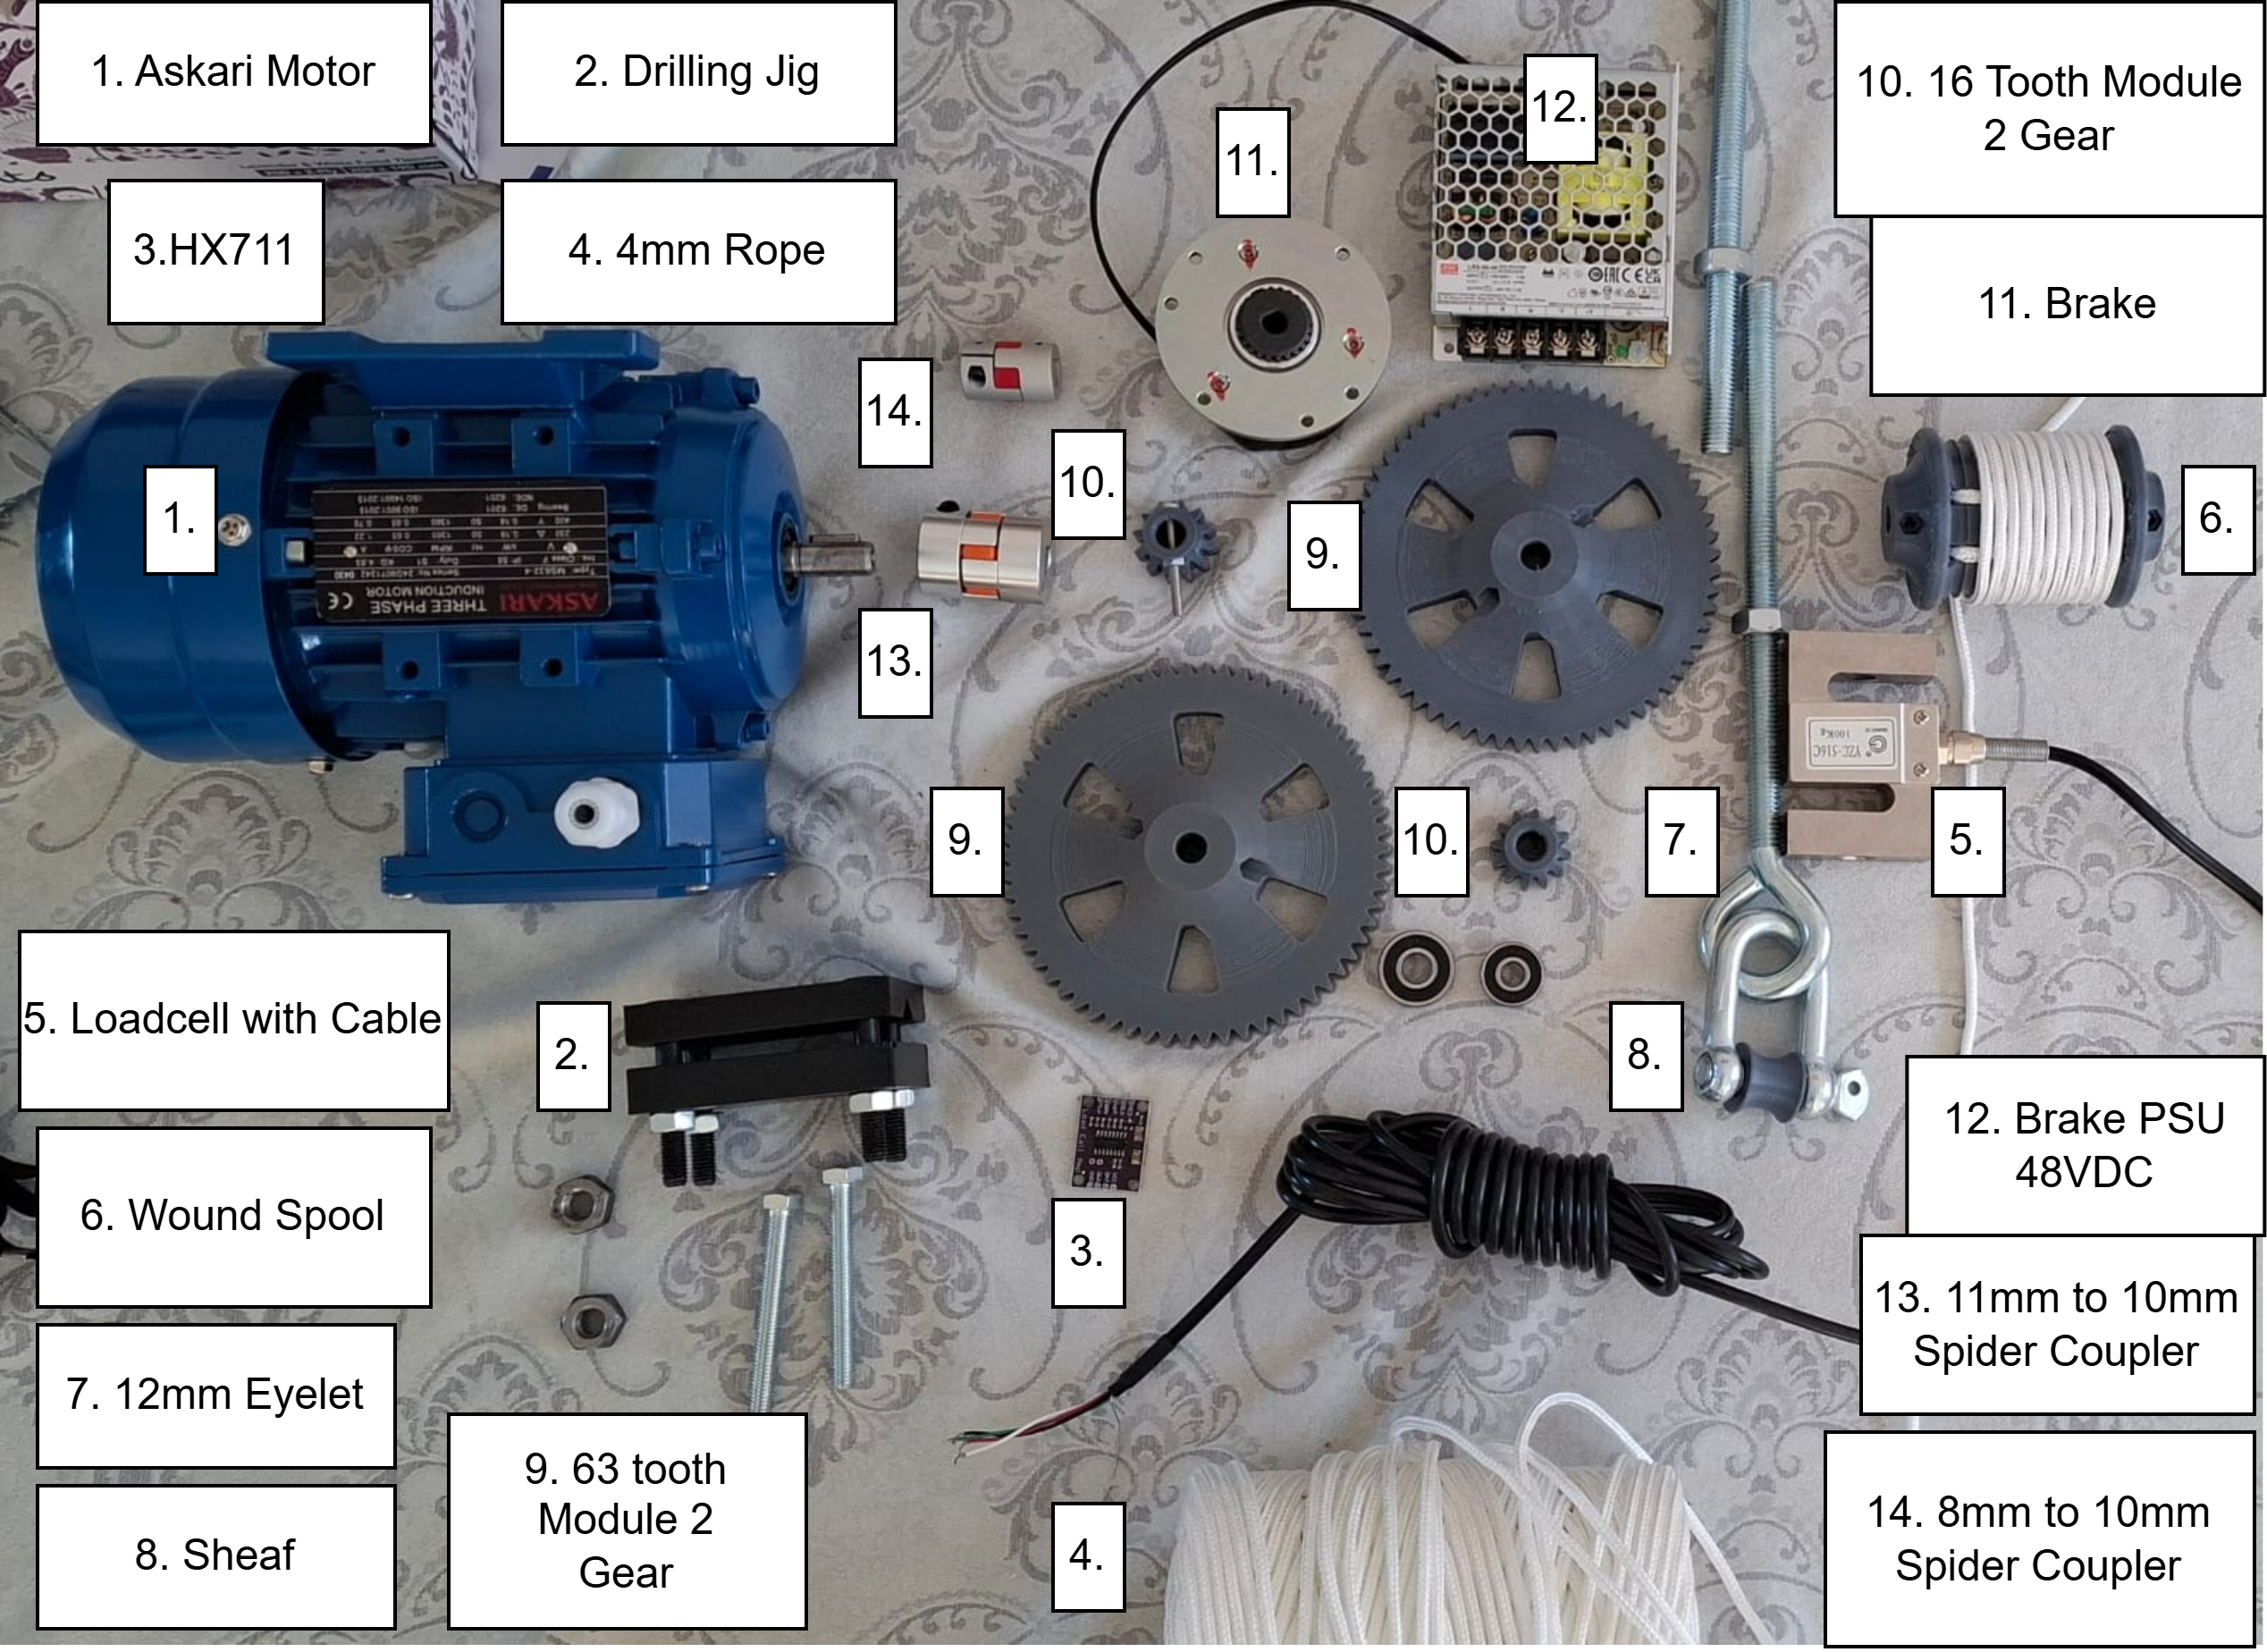
\includegraphics[width=0.8\textwidth]{figures/Fig_Components_and_Parts_MCTRII.png}
    \caption{All Components for MCTR II Up to Date of Report Publication.}
    \label{fig:mctr-ii-implementation}
\end{figure}

The main components in this iamge are those that have been acquired up to date. The mild steel rods had been acquired within the week of writing this report and thus still need to be processed. In the image each of the components are numbered and named with the most prominent designed components the 4 gears to be used in the 2 stages in that configuration, with the gear at ~10. showing the method that will be used to fasten it to the shaft with a throughhole bolt and nut. The other gears will be fastened likewise. The eyebolts will be cut to size and used to fasten to MCTR I

\subsection{Engineering Drawings and Supporting Evidence}

Supporting evidence may include CAD drawings, component
specifications, assembly photographs, and other records that
demonstrate how MCTR II was constructed.

\begin{figure}[H]
    \centering
    % \includegraphics[width=0.8\textwidth]
    % {img/mctr_ii_design}
    \caption{Engineering drawing or CAD representation of MCTR II.}
    \label{fig:mctr-ii-design}
\end{figure}

\section{REII Implementation Evidence}
\label{sec:reii-evidence}
\label{sec:sw-impl}

This section presents the available evidence from earlier
REII hardware testing and software development.
Implementation of the final ESP32-S3 crane system remains
incomplete.

\subsection{Physical Implementation}

Figure~\ref{fig:reii-implementation} shows the earlier
radio bench comprising two ESP32 boards and two nRF24
modules. Later bench firmware generated physical PWM
outputs while motion and sensor readings were simulated.
The current controller is the university-supplied
ESP32-S3 board, which still requires firmware migration
and crane integration.

\begin{figure}[H]
    \centering
    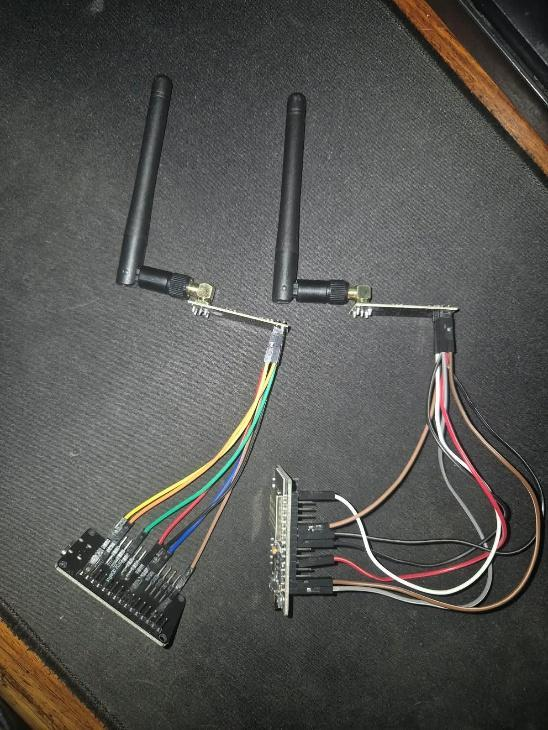
\includegraphics[width=0.32\textwidth]
        {figures/Figure_8_9_Radio_Assembly.jpg}
    \caption{Earlier two-ESP32/nRF24 radio bench assembly.}
    \label{fig:reii-implementation}
\end{figure}

\subsection{Supporting Design Evidence}

Figure~\ref{fig:reii-design} shows the proposed software
arrangement linking the Python dashboard, STM32 ground
station and ESP32-S3 controller. The existing dashboard,
STM32 bridge and earlier ESP32 controller software would
provide the basis for this implementation.

The Excel workbook records the earlier radio measurements.
\cite{reii_measurements2026}
Migration to the ESP32-S3 and integrated testing of the
sensors, brake and complete crane remain outstanding.

\begin{figure}[H]
    \centering
    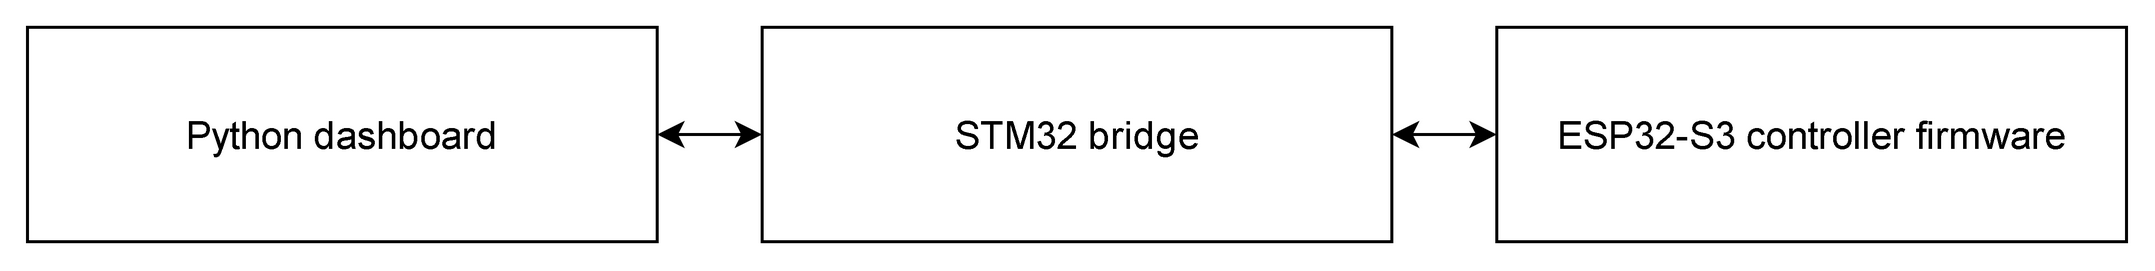
\includegraphics[width=0.95\textwidth]
        {figures/Figure_8_10_Software_Sources.png}
    \caption{Proposed REII software arrangement.
        ESP32-S3 migration remains incomplete.}
    \label{fig:reii-design}
\end{figure}

\section{Integrated System Implementation}
\label{sec:integrated-system-evidence}

This section demonstrates how the five subsystems were assembled
and integrated into the complete gantry crane system. The evidence
should show the overall arrangement and the interfaces between
the subsystems.

\subsection{Final Assembly}

Figure~\ref{fig:integrated-system-evidence} presents the assembled
gantry crane.

\begin{figure}[H]
    \centering
    % \includegraphics[width=0.85\textwidth]
    % {img/integrated_system}
    \caption{Completed gantry crane system.}
    \label{fig:integrated-system-evidence}
\end{figure}

The figure should demonstrate the overall arrangement of the
implemented system and identify the locations of EERI I, EERI II,
MCTR I, MCTR II, and REII. Multiple views may be provided where
necessary to show interfaces that cannot be seen in a single
photograph.

\subsection{Subsystem Interfaces}

The subsystem interfaces shall be documented using appropriate
photographs, assembly drawings, wiring diagrams, or interface
schematics. These records should show how the subsystems are
physically and functionally connected.

\begin{figure}[H]
    \centering
    % \includegraphics[width=0.85\textwidth]
    % {img/system_interfaces}
    \caption{Interfaces between the implemented subsystems.}
    \label{fig:system-interfaces}
\end{figure}

The evidence should be consistent with the subsystem interface
matrix in Chapter~\ref{ch:system-performance}, or the relevant
chapter in which the interface analysis is presented. Any
modifications made during integration should be documented.

\section{Implementation Evidence Summary}
\label{sec:implementation-evidence-summary}

Table~\ref{tab:implementation-evidence-summary} summarises the
evidence provided for each subsystem and the integrated system.

\begin{table}[H]
    \centering
    \caption{Summary of implementation evidence.}
    \label{tab:implementation-evidence-summary}
    \renewcommand{\arraystretch}{1.4}
    \begin{tabularx}{\textwidth}{|X|X|X|}
        \hline
        \textbf{Subsystem} &
        \textbf{Evidence provided} &
        \textbf{Implementation status} \\
        \hline
        EERI I &
        [Photographs, drawings, schematics, or other evidence] &
        [Completed / Partial / Not implemented] \\
        \hline
        EERI II &
        [Photographs, drawings, schematics, or other evidence] &
        [Completed / Partial / Not implemented] \\
        \hline
        MCTR I &
        [Photographs, CAD drawings, assembly records, or other evidence] &
        [Completed / Partial / Not implemented] \\
        \hline
        MCTR II &
        [Photographs, CAD drawings, assembly records, or other evidence] &
        [Completed / Partial / Not implemented] \\
        \hline
        REII &
        [Photographs, drawings, schematics, or other evidence] &
        [Completed / Partial / Not implemented] \\
        \hline
        Integrated system &
        [Overall assembly photographs and interface evidence] &
        [Completed / Partial / Not implemented] \\
        \hline
    \end{tabularx}
\end{table}

The evidence presented in this chapter documents the extent to
which the design has been implemented. The implementation records
provide a basis for interpreting the performance results presented
in Chapter~\ref{ch:system-performance}. Evidence of physical
construction alone does not establish that the system meets its
performance requirements; this must be demonstrated by the
relevant verification and validation results.

% ============================================================
%  CHAPTER 9 – CONCLUSION
% ============================================================
\chapter{Conclusion}
\label{ch:conclusion}

This report has documented the engineering design process for the gantry crane, including the development of a proposed design in response to the project requirements. The work presented establishes a foundation for completing and evaluating the system.

The design must still be validated before it is implemented. Further work should verify the calculations and component selections against the final requirements, assess the structural and operational performance, and test the assembled crane for safe and reliable operation. Any required design changes, verification results and test findings should be incorporated into the next revision of this report.

% ── References ──────────────────────────────────────────────
\newpage
\printbibliography[heading=bibintoc, title={References}]

% ── Appendices ──────────────────────────────────────────────
\newpage
\appendix
%% ============================================================
%  APPENDIX A – GENERATIVE AI USAGE LOG
% ============================================================
\chapter{Generative AI Usage}
\label{app:ai-usage}

[List every instance where generative AI tools were used to assist
in writing or editing any part of this report, as required by the
Declaration of Originality.]

\begin{table}[H]
    \centering
    \caption{Generative AI (GA) evidence throughout the report.}
    \label{tab:ga-evidence}
    \begin{tabular}{@{} l l p{3.5cm} p{4.5cm} @{}}
        \toprule
        \textbf{Section} & \textbf{Tool} & \textbf{Prompt summary}
            & \textbf{How output was used} \\
        \midrule
        \S\ref{sec:sw-impl} & ChatGPT-4o
            & ``Explain threading model for \ldots''
            & Edited, verified, and rewritten in own words. \\
        \bottomrule
    \end{tabular}
\end{table}

% ============================================================
%  APPENDIX B – RISK REGISTER
% ============================================================
\chapter{Risk Register}
\label{app:risk}

\begin{figure}[H]
    \centering
    \includegraphics[width = 0.75\textwidth]{App_RiskEvaluation_Matrix.png}
    \caption{Risk Evaluation Matrix used to determine risk severity \cite{Risk_Eval_Table}.}
    \label{app:risk-eval-table}
\end{figure}


\rowcolors{1}{gray!25}{white}
\begin{table}[H]
    \centering

    \caption{Risk identification and management.}
    \label{tab:risk-register}
    \begin{tabular}{@{} l p{4cm} p{4.5cm} p{8cm} @{}}
        \toprule
        \textbf{ID} & \textbf{Risk description}
                    & \textbf{Likelihood and Impact}
                    & \textbf{Mitigation strategy}                                                                    \\
        \midrule
        S1          & Late Component Delivery
                    & Possible; Significant
                    & Determine and order components 2 weeks ahead of time; look for local suppliers.                 \\
        S2          & Component Failure
                    & Likely; Significant
                    & Acquire spares where reasonable and obtain quality suppliers.  \\
        G1          & Member does not adhere to responsibilities
                    & Possible; Significant
                    & Perform weekly check-ins, work management, and performance measures.                            \\
        G2          & Member's attention required elsewhere, e.g. death or disaster.
                    & Possible; Severe
                    & Communicate possible interferences with group responsibilities and plan accordingly.            \\
        K1          & Tool ignorance e.g. CAD, Simulink, Git, Codebase.
                    & Very Likely; Significant                                                                                      
                    & Share knowledge of tools with other members and learn from tutorials as required.               \\
        K2          & Ignorance regarding components
                    & Very Likely; Significant                                                                                     
                    & Rely on familiar experience and components; consult resources to learn of new ones required.    \\
        P1          & Integration failure of subsystems 
                    & Possible, Severe
                    & Have clear documentation of subsystems, tests and confirmation during development.                                \\
        L1          & Workshop / Lab Access Conflicts 
                    & Very Likely; Significant
                    & Make use of members' tools or organise with other acquantances who have 3D printers or fabrication facilities. \\
        L2          & Poor Documentation and Traceability Problems          
                    & Very Likely; Significant 
                    & Use shared GitHub repository with version control of all files and drawings with naming conventions.   \\
        \bottomrule
    \end{tabular}
\end{table}

\begin{table}[H]
    \centering
    \caption{Risk traceability matrix \textbf{BEFORE} mitigation.}
    \label{tab:risk-before}
    \renewcommand{\arraystretch}{1.4}
    \begin{tabular}{@{} l | c c c c c @{}}
        \toprule
                            & \multicolumn{5}{c}{\textbf{Impact}}                                                    \\
        \textbf{Likelihood} & \textbf{1 – Negligible}             & \textbf{2 – Minor}
                            & \textbf{3 – Moderate}               & \textbf{4 – Major} & \textbf{5 – Severe}         \\
        \midrule
        5 – Very high       &                                     &                    &                     &     & \\
        4 – High            &                                     &                    &                     & R01 & \\
        3 – Medium          &                                     &                    & R03                 &     & \\
        2 – Low             &                                     &                    &                     & R02 & \\
        1 – Very low        &                                     &                    &                     &     & \\
        \bottomrule
    \end{tabular}
\end{table}

\begin{table}[H]
    \centering
    \caption{Risk traceability matrix \textbf{AFTER} mitigation.}
    \label{tab:risk-after}
    \renewcommand{\arraystretch}{1.4}
    \begin{tabular}{@{} l | c c c c c @{}}
        \toprule
                            & \multicolumn{5}{c}{\textbf{Impact}}                                                 \\
        \textbf{Likelihood} & \textbf{1 – Negligible}             & \textbf{2 – Minor}
                            & \textbf{3 – Moderate}               & \textbf{4 – Major} & \textbf{5 – Severe}      \\
        \midrule
        5 – Very high       &                                     &                    &                     &  & \\
        4 – High            &                                     &                    &                     &  & \\
        3 – Medium          &                                     & R01                & R02                 &  & \\
        2 – Low             &                                     & R03                &                     &  & \\
        1 – Very low        &                                     &                    &                     &  & \\
        \bottomrule
    \end{tabular}
\end{table}

% !TEX root = ../main.tex
% ============================================================
%  APPENDIX C – ADDITIONAL TECHNICAL DATA
% ============================================================
\chapter{Additional Technical Data}
\label{app:technical}

\section{EERI II: Magnetic Load Attachment}
\label{sec:app-eeri2-technical}
This section details the physical dimensions, electrical loop parameters, and governing analytical equations for the EERI II magnetic load attachment subsystem.

\subsection{Electromagnet Coil and Circuit Specifications}
Table~\ref{tab:app_eeri2_specs} summarises the complete mechanical, electrical, and magnetic design parameters for the custom hand-wound bobbins.

\begin{table}[H]
  \centering
  \caption{EERI II Electromagnet Coil and Circuit Specifications.}
  \label{tab:app_eeri2_specs}
  \begin{tabular}{|l|r|l|l|}
    \hline
    \multicolumn{4}{|c|}{\textbf{Electromagnet Design Specifications}} \\
    \hline
    \textbf{Parameter} & \textbf{Value} & \textbf{Unit} & \textbf{Comment / Derivation} \\
    \hline
    Payload Mass & 20.0 & kg & Maximum specified test payload \\
    Required Retention Force ($F_g$) & 196.2 & N & $m \cdot g$ ($g = 9.81\,\text{m/s}^2$) \\
    Attachment Points & 3 & ul & U-core geometry with 2 poles each \\
    Total Spools & 6 & ul & 2 spools per U-core point \\
    Core Diameter ($\Phi_{\mathrm{core}}$) & 20.0 & mm & 1018 structural steel core \\
    Flange Diameter ($\Phi_{\mathrm{flange}}$) & 40.0 & mm & 3D-printed bobbin outer limit \\
    Winding Length ($h_{\mathrm{wind}}$) & 50.0 & mm & Axial bobbin winding window \\
    Radial Winding Depth ($d_{\mathrm{rad}}$) & 10.0 & mm & $(40 - 20)/2\,\text{mm}$ \\
    Wire Outer Diameter ($d_{\mathrm{OD}}$) & 1.00 & mm & AWG 19/20 enamelled copper wire \\
    Bare Conductor Diameter ($d_{\mathrm{Cu}}$) & 0.94 & mm & Copper cross-section $0.694\,\text{mm}^2$ \\
    Turns per Layer ($N_{\mathrm{layer}}$) & 48 & turns & $\approx 50\,\text{mm} / 1.0\,\text{mm}$ \\
    Number of Layers & 6 & layers & Radial build $6.0\,\text{mm} \le 10.0\,\text{mm}$ \\
    Total Turns per Spool ($N$) & 286 & turns & Hand-wound layer wound \\
    Mean Turn Circumference ($C_{\mathrm{mean}}$) & 94.25 & mm & $\pi \times 30.0\,\text{mm}$ \\
    Wire Length per Spool ($L_{\mathrm{spool}}$) & 28.0 & m & Including flying connection leads \\
    Total Copper Wire Length & 168.0 & m & 6 spools in series \\
    Single Spool Resistance ($20^\circ\text{C}$) & 0.72 & $\Omega$ & Measured cold DC resistance \\
    Total Series Resistance ($20^\circ\text{C}$) & 4.32 & $\Omega$ & Measured series loop cold \\
    Total Loop Resistance ($50^\circ\text{C}$) & 4.95 & $\Omega$ & Warm copper + MOSFET + harness \\
    Rail Voltage ($V_{\mathrm{boost}}$) & 13.5 & V & Sized to guarantee 2.80\,A warm \\
    Operating Current ($I_{\mathrm{op}}$) & 2.80 & A & Sustained continuous excitation \\
    MMF per Spool ($N \cdot I$) & 800.8 & A-t & Ampere-turns per coil \\
    MMF per U-Core Point & 1601.6 & A-t & 2 spools in series \\
    Power Dissipation per Spool & 5.64 & W & Continuous conduction \\
    Total Magnet System Power & 33.84 & W & 6 spools energized \\
    Core Flux Density ($B_{\mathrm{core}}$) & 1.32 & T & 2D planar FEMM simulation \\
    Holding Force per Point ($F_y$) & 89.56 & N & At $0.20\,\text{mm}$ parasitic air gap \\
    Total Static Holding Force ($F_{\mathrm{total}}$) & 268.68 & N & $3 \times 89.56\,\text{N}$ ($27.39\,\text{kg}$) \\
    Safety Factor & 1.37 & ul & $268.68\,\text{N} / 196.2\,\text{N}$ ($+37\%$ margin) \\
    \hline
  \end{tabular}
\end{table}

\section{MCTR II: Spooling}
These are all the relevant technical data pertaining to the MCTR II work package.

\subsection{Spreadsheets and Tables}
Additional excel calculations, data and equations used for relevant calculations.
% Table generated by Excel2LaTeX from sheet 'Sheet1'
\begin{table}[H]
  \centering
  \caption{Design main specifications}
  \begin{tabular}{|r|r|l|}
    \hline
    \multicolumn{3}{|c|}{\textbf{Design Main Specifications}} \\
    \hline
    \multicolumn{1}{|l|}{Max Load} & 30 & kg \\
    \multicolumn{1}{|l|}{Stroke} & 1600 & mm \\
    & 80 & mm/s \\
    \hline
  \end{tabular}
  \label{tab:design_main_specs}
\end{table}

% Table generated by Excel2LaTeX from sheet 'Sheet1'
\begin{table}[H]
  \centering
  \caption{Gear specifications}
  \begin{tabular}{|l|r|l|l|}
    \hline
    \multicolumn{4}{|c|}{\textbf{Gear Specs}} \\
    \hline
    \textbf{Parameter} & \textbf{Value} & \textbf{Unit} & \textbf{Comment} \\
    \hline
    Module & 2 & ul & \\
    Number\_of\_Teeth & 30 & ul & \\
    Pressure\_Angle & 25 & deg & \\
    Gear\_Height & 15 & mm & \\
    Pitch\_Circle & 60 & mm & \\
    Addendum\_Circle & 64 & mm & \\
    Root\_Circle & 55 & mm & \\
    Clearance\_Circle & 56 & mm & \\
    Base\_Circle & 54.37847 & mm & \\
    \hline
    Reduction Ratio & 44.5059 & & \\
    Per Stage work & 6.671274 & & \\
    Np & 11 & & \\
    Ng & 250 & & \\
    m & 22.72727 & & \\
    \hline
  \end{tabular}
  \label{tab:gear_specs}
\end{table}

% Table generated by Excel2LaTeX from sheet 'Sheet1'
\begin{table}[H]
  \centering
  \caption{Drum specifications}
  \begin{tabular}{|l|r|l|}
    \hline
    \multicolumn{3}{|c|}{\textbf{Drum Specs}} \\
    \hline
    Line Speed & 88 & mm/s \\
    Diameter & 50 & mm \\
    Height & 60 & mm \\
    Starting Serving Factor & 1,5 & \\
    Circumference & 157.0796 & mm \\
    Loops of Circ fitted & 12 & \\
    Rope Length in 1 layer & 1884.956 & \\
    Rpm & 30.55775 & \\
    Torque & 11.03625 & Nm \\
    \hline
  \end{tabular}
  \label{tab:drum_specs}
\end{table}

% Table generated by Excel2LaTeX from sheet 'Sheet1'
\begin{table}[H]
  \centering
  \caption{Rope specifications}
  \begin{tabular}{|l|r|l|}
    \hline
    \multicolumn{3}{|c|}{\textbf{Rope Specs}} \\
    \hline
    Diameter & 5 & mm \\
    Length & 1600 & mm \\
    Wraps & 10.18592 & \\
    \hline
  \end{tabular}
  \label{tab:rope_specs}
\end{table}

% Table generated by Excel2LaTeX from sheet 'Sheet1'
\begin{table}[H]
  \centering
  \caption{Three-phase motor specifications}
  \begin{tabular}{|l|r|l|}
    \hline
    \multicolumn{3}{|c|}{\textbf{3-Phase Motor Specs}} \\
    \hline
    Power & 0.18 & kW \\
    Speed & 1360 & rpm \\
    Mass & 4.83 & kg \\
    Shaft & 11 & mm \\
    Keyway & 4*16 & mm \\
    Rated Torque & 1.263877 & Nm \\
    Starting Torque & 3.791632 & Nm \\
    \hline
  \end{tabular}
  \label{tab:motor_specs}
\end{table}

\subsection{Equations}
\label{subsec:c-equations}

\begin{equation}
\label{eq:drum_torque}
\tau_{\mathrm{Drum}} = \mathrm{Load} \times 9.81 \times \frac{\varnothing_{\mathrm{Drum}}}{2 \times 1000} \times K_{\mathrm{Serving\ Factor}}
\end{equation}

\begin{equation}
\label{eq:min_gear}
\mathrm{N_P} = \frac{2\mathrm{k}}{(1 + 2\mathrm{m})\sin^2 \phi} \left( \mathrm{m} + \sqrt{\mathrm{m}^2 + (1 + 2\mathrm{m})\sin^2 \phi} \right)\end{equation}

\begin{equation}
\label{eq:max_gear}
\mathrm{N_G} = \frac{\mathrm{N_P}^2 \sin^2 \phi - 4k^2}{4k - 2N_P \sin^2 \phi}
\end{equation}

\begin{equation}
\label{eq:pitch_circle}
D_P = \mathrm{module} \times \mathrm{z}
\end{equation}

\begin{equation}
\label{eq:gear_module}
\mathrm{D} = \frac{p}{\pi}
\end{equation}


\begin{equation}
\label{eq:addendum_circle}
D = D_p + 2 \times m
\end{equation}


\begin{equation}
\label{eq:root_circle}
D_r = D_p - 2 \times b
\end{equation}


\begin{equation}
\label{eq:dedendum}
b = 1.25 \times m
\end{equation}

\begin{equation}
\label{eq:clearance_circle}
D_c = D_p - 2\times m
\end{equation}


\begin{equation}
\label{eq:circular_pitch}
p = m\times\pi
\end{equation}

\begin{equation}
\label{eq:base_circle}
D_b = D_p \cos{\alpha}
\end{equation}

\begin{equation}
    \label{eq:rig_torque}
    \tau = F \times d
\end{equation}

\textbf{Subsystem function:} Raise and lower a payload of up to \InMassRated\,kg through
a \InStroke\,m stroke on a rope and drum, hold it without drift when power or command is
lost, and report the on-hook load to the controller (FR4, FR5, FR6, PT2).
 
\textbf{Test setup:} Complete hoist assembly (motor, coupling, gearbox, brake, drum, rope,
load cell with sheave, HX711) bolted to the test frame; VSD or bench supply for the motor;
48\,V brake supply and relay; controller or bench read-out of the HX711; calibrated
reference masses (5, 10, 20, 30\,kg); stopwatch or encoder for timing; tape measure for drift.
Protect the area below the load. The 30\,kg proof test is performed last.
 
\begin{table}[htbp]
    \centering
    \caption{MCTR II test plan}
    \label{tab:appendix-mctr-ii-tests}
    \small
    \renewcommand{\arraystretch}{1.4}
    \begin{tabularx}{\textwidth}{|l|X|X|X|X|}
        \hline
        \textbf{Test ID} &
        \textbf{Test description} &
        \textbf{Procedure} &
        \textbf{Expected result} &
        \textbf{Status} \\
        \hline
        MCII-01 & Functional: raise and lower (FR4) &
        Command raise then lower with \InMassRated\,kg over the full stroke. &
        Moves in the commanded direction over the full \InStroke\,m without slip or rope overlap. &
        [Pass/Fail/NT] \\
        \hline
        MCII-02 & Performance: hoist rate (PT2) &
        Time a full-stroke raise with \InMassRated\,kg at the VSD frequency available. &
        Stroke time $\le \InTimeReq$\,s; predicted \showv{Tstroke}{1}{s} at \InVsdF\,Hz. &
        [Pass/Fail/NT] \\
        \hline
        MCII-03 & Safety: fail-safe brake (FR6) &
        Hold \InMassRated\,kg mid-stroke, remove brake power, then remove command signal. &
        Brake engages; drift $\le$ \tbd{mm} in \tbd{min}. &
        [Pass/Fail/NT] \\
        \hline
        MCII-04 & Functional: load feedback (FR5) &
        Hang 0, 5, 10, 20, 30\,kg and record the HX711 reading; fit a two-point calibration. &
        Reading within \tbd{\%} of the reference mass over the range; resolution about \showv{ResG}{0}{g}. &
        [Pass/Fail/NT] \\
        \hline
        MCII-05 & Safety: overload interlock &
        Raise a mass above the trip level of \showv{Mtrip}{1}{kg}. &
        Raising stops and the brake engages within \showv{Latency}{0}{ms}. &
        [Pass/Fail/NT] \\
        \hline
        MCII-06 & Performance: structural proof &
        Hold \InMassDesign\,kg statically for 60\,s on the rig. &
        No visible deformation or tooth damage; shaft safety factor $\ge$ \InSFreq\ in Appendix~\ref{app:technical}. &
        [Pass/Fail/NT] \\
        \hline
        MCII-07 & Performance: gear test pair &
        Load a printed stage~B pair in the rig through a torque arm to failure. &
        Failure torque gives the measured allowable stress replacing \InSigAllow\,MPa. &
        [Pass/Fail/NT] \\
        \hline
    \end{tabularx}
\end{table}

\clearpage
\section{REII Preliminary ESP32 Radio Tests}
\label{sec:reii-radio-tests}

These earlier tests used two original ESP32 development
boards and nRF24L01 radios, before the final ESP32-S3
course-board integration. They support
Section~\ref{sec:reii-subsystem-remote-control-dashboard}
but do not establish final S3 or crane performance.
Figure~\ref{fig:reii-implementation} shows the temporary
assembly.
\cite{reii_measurements2026}

\noindent
\textbf{Test method:}
The tests used the TMRh20 RF24 library, regulated 3.3~V
radio supplies, and fixed antenna orientation and height
in the same laboratory. Each condition had two trials
of 1000 sequentially numbered packets.
Table~\ref{tab:reii-radio-measurements} retains each
trial's received count; mean packet loss is calculated
from 2000 sent packets per condition. ACK-on tests
allowed up to three retries with a
1000~$\mu$s retry delay.

\begin{table}[H]
    \centering
    \footnotesize
    \renewcommand{\arraystretch}{1.1}
    \setlength{\tabcolsep}{3pt}
    \caption{Earlier ESP32 radio measurements.}
    \label{tab:reii-radio-measurements}

    \begin{tabularx}{\textwidth}{@{}
        *{7}{>{\centering\arraybackslash}X}
    @{}}
        \toprule
        \textbf{Distance}\newline (m) &
        \textbf{Rate}\newline (kbps) &
        \textbf{Channel} &
        \textbf{ACK /}\newline \textbf{max retries} &
        \textbf{Received}\newline \textbf{trial 1} &
        \textbf{Received}\newline \textbf{trial 2} &
        \textbf{Mean loss}\newline (\%) \\
        \midrule

         1 &  250 & 76 & Off / 0 &  997 &  907 &  4.80 \\
         1 & 2000 & 76 & Off / 0 &  971 &  985 &  2.20 \\
         2 &  250 & 76 & Off / 0 &  984 &  901 &  5.75 \\
         2 & 2000 & 76 & Off / 0 &  987 &  976 &  1.85 \\
         4 &  250 & 76 & Off / 0 &  992 &  974 &  1.70 \\
         4 & 2000 & 76 & Off / 0 &  956 &  977 &  3.35 \\
         8 &  250 & 76 & Off / 0 &  997 &  937 &  3.30 \\
         8 & 2000 & 76 & Off / 0 &  942 &  970 &  4.40 \\
        12 &  250 & 76 & Off / 0 &  953 &  960 &  4.35 \\
        12 & 2000 & 76 & Off / 0 &  942 &  939 &  5.95 \\
        16 &  250 & 76 & Off / 0 &  970 &  853 &  8.85 \\
        16 & 2000 & 76 & Off / 0 &  897 &  877 & 11.30 \\
        \midrule

         8 &  250 & 12 & Off / 0 &  836 &  842 & 16.10 \\
         8 & 2000 & 12 & Off / 0 &  970 &  920 &  5.50 \\
        \midrule

         1 &  250 & 76 & On / 3 & 1000 & 1000 & 0.00 \\
         1 & 2000 & 76 & On / 3 & 1000 & 1000 & 0.00 \\
        16 &  250 & 76 & On / 3 & 1000 & 1000 & 0.00 \\
        16 & 2000 & 76 & On / 3 & 1000 &  999 & 0.05 \\

        \bottomrule
    \end{tabularx}
\end{table}

\noindent
\textbf{Findings:}
With ACK disabled on channel 76, 250~kbps had lower mean
packet loss than 2~Mbps at the tested distances from
4 to 16~m. With acknowledgements and retries enabled,
both 250~kbps trials received all 1000 packets at
1~m and 16~m. Variation between repeated trials limits
generalisation.
\cite{reii_measurements2026}

\noindent
\textbf{Limitations:}
The workbook records 0~dBm throughout; the current
runtime power setting (code 2) was not compared.
No latency measurements were recorded. Final S3
communication, response time and integrated fault
behaviour remain unvalidated.

\end{document}
